\documentclass[twoside,a4,12p]{report} %,draft,openright]

% packages
\usepackage{epsf,
			epstopdf,
			graphicx, 
			latexsym,
			amssymb,
			anysize, % for margins left, right top bottom
			setspace,
			cite,
			fancyhdr, %does the headers on the pages - keep in
			amsmath,
			algorithm,
			url,
			hyperref,
			algorithm,
			algorithmic,
			subfigure
			}
\marginsize{4cm}{2.5cm}{4cm}{4cm}

%\usepackage{draft} %draft option - doesn't put full figures in -
                   % useful when editing

%omitting any of these makes the thesis compile without the omitted
%chapter - good for editing single chapters.
%\includeonly{header,intro,problem-def, state-of-the-art, methodology, results, appendix}

%%%%% my add-ons %%%%%
\newcommand{\vect}[1]{\boldsymbol{#1}}
%%%%%%%%%%%%%%%%%%%%%%
\begin{document}

\newpage

%Puts page numbering of preamble in roman and of main body of thesis in
%arabic. Also defines how chapters and sections are made
\pagenumbering{arabic}
\setcounter{page}{1} \pagestyle{fancy}
\renewcommand{\chaptermark}[1]{\markboth{\chaptername%
\ \thechapter:\,\ #1}{}}
\renewcommand{\sectionmark}[1]{\markright{\thesection\,\ #1}}

%DEFINES TITLE PAGE, and contains abstract, acknowledgements, etc.

%%%%%%%%%%%%%%%%%%%%%%%%%%%%%%%%%%%%%%%%%%%%%%%%%%%%%%%%%%%%%%%%%%%%%%%%%%%
% This is a sample header for a sample dissertation. Fill in the name,
% and the other information. LaTeX will work out the table of
% content, the list of figures and of tables for you.
%%%%%%%%%%%%%%%%%%%%%%%%%%%%%%%%%%%%%%%%%%%%%%%%%%%%%%%%%%%%%%%%%%%%%%%%%%%

\newpage
\thispagestyle{empty}

% ******* Title page *******
% **************************

\vspace*{2cm}
\begin{center}
{\Large\bf Underwater vehicle localisation using Extended Kalman Filter\\} \vspace{2cm} {\large
Author: Miroslav Radojevi\'c \\
Supervisor: Yvan Petillot    \\
\vspace{3cm}
Ocean Systems Lab \\
Heriot-Watt University, Edinburgh  \\
\vspace{0.5cm}
Escola Polit\`{e}cnica Superior \\
Universitat de Girona \\ 
\vspace{0.5cm}
Centre Universitaire Condorcet \\
Universit\'{e} de Bourgogne  
}

\end{center}

\vspace{3.5cm}
\begin{center}
{\large A Thesis Submitted for the Degree of \\MSc Erasmus Mundus
in Vision and Robotics (VIBOT) \\\vspace{0.3cm} $\cdot$ 2011
$\cdot$}
\end{center}
\singlespacing


%ABSTRACT
\begin{abstract}
In order to accomplish various missions, autonomous underwater vehicles need to be capable of estimating their position within the environment. This is a prerequisite of a successful mission since further tasks that need to be achieved strongly rely on navigation information as a source of valuable information. Much has been said about navigation underwater, yet the research has not reached the level of having as equally precise solution for navigation as the one available above the water surface.  

This thesis is a study on application of an algorithm that would accomplish the localisation of the Ocean Systems Lab's Nessie underwater vehicle using measurements from a number of sensors mounted on it. Well known Extended Kalman Filter (EKF) algorithm approach was suggested as a solution for robot self-localisation. Chosen method uses measurements from the set of sensors installed on the vehicle. Standard Kalman Filtering routine involves two stages: prediction and correction. Prediction model is derived from the mathematical model of the vehicle dynamics. Based on the laws of kinematics, prediction model calculates the next vehicle dynamic state. Five degrees of freedom (d.o.f.) \textit{constant-speed} model for motion of the rigid body was proposed for this purpose. Measurements from different sensors are fused together to make the observations. Observations are responsible for the correction stage. In other words, observations have been combined together with the process model in order to make a quality estimate of the current location of the robot within the environment. 

Prediction model applies the laws of physics in order to make a suitable role model of robot movement. Inspiration for the solution comes from previous works on EKF-based localisation. Practical application of the EKF implies management of the observations in terms of time and sensor type. Additional practical issue that was addressed in the thesis is the choice of heading sensor and quality of obtained heading as an important ingredient of the navigation. Implementation of Unscented Kalman Filter (UKF) was investigated as potential improvement in working with nonlinearities. Finally, the absolute position observations tend to be quite noisy, nevertheless very important navigation measurements. EKF was demonstrated as a tool for sensor fusion and simultaneous filtering of the position measurements.     

In addition, the work gives a summary of the underwater localisation methods and capabilities. Theoretical background on nonlinear filtering was investigated in order to justify the reasons for choosing EKF. Finally, experiments with recorded sensor data and some real missions have been carried out. Their results have been presented as a part of navigation performance test and analysis.% of the characteristics of the localisation. 
%Introduction summarizes possible methods and obstacles arising from the nature of the underwater environment and sensor features.%Second part goes deeper into the matter explaining practical solution for navigation and the details of the implementation together with the issues that needed to be solved. Eventually, an analysis of the results is offered. Preliminary computer simulations and, eventually, the authentic results recorded from the real missions. 
%together with the authentic real mission results
The emphasis is on the engineering of the solution, improving the navigation and finding the way to overcome known deficiencies, mostly due to nonlinearities, volatile heading measurement and measurement imprecisions. Thesis is intended to report pros and cons of a practical piece of work, implemented in C++ within the Robot Operating System (ROS) framework and Nessie software and hardware platform - where a scientific concept was adopted to solve the real task. 
\vspace*{16cm}



%\begin{center}
%\begin{quote}
%\it Research is what I'm doing when I don't know what I'm
%doing.\,\ldots
%\end{quote}
%\end{center}
%\hfill{\small Werner von Braun}
\begin{center}
\begin{quote}
%\it Prediction is difficult - especially of the future.\,\ldots
\it If one does not know to which port one is sailing, no wind is favourable.
\end{quote}
\end{center}
%\hfill{\small Attributed to Niels Henrik David Bohr (1885-1962)}
\hfill{\small Seneca, Roman philosopher, mid-1st century AD}

\end{abstract}

\doublespacing

%\pagestyle{empty}
\pagenumbering{roman}
\setcounter{page}{1} \pagestyle{plain}


\tableofcontents

\listoffigures
\listoftables

\chapter*{Acknowledgments}
\addcontentsline{toc}{chapter}
         {\protect\numberline{Acknowledgments\hspace{-96pt}}}

I would like to thank European Commission for financing and VIBOT consortium for giving me opportunity to participate in the program. It's been a valuable experience to live and study all across the Europe past two years. I am grateful to my course colleagues for the memorable moments and help, university staff and administration and Ocean Systems Lab for being an inspiring environment. I express special gratitude to my thesis supervisor Yvan for all the advice and the time spent solving problems,  and to Joel for his patience and knowledge.  
Finally, I am grateful my family who has been an honest support and a true friend all this time.       
\pagestyle{fancy}


\newpage

%sets up headers for lefthand and righthand pages. To alter, edit
%these lines and the chaptermark/sectionmark lines above
\addtolength{\headheight}{3pt} \fancyhead{}
\fancyhead[LE]{\sl\leftmark} \fancyhead[LO,RE]{\rm\thepage}
\fancyhead[RO]{\sl\rightmark} \fancyfoot[C,L,E]{}
\pagenumbering{arabic}

%\singlespacing
%\doublespacing
\onehalfspacing

\chapter{Introduction} \label{chap:intro}

\section{Why underwater?} \label{sect:thefirst}

Manhood has managed to conquer variety of environments. At some point, humans could walk on the moon, send expeditions to cold or remote areas in different corners of the planet. Sea-floor constitutes the largest part of Earth's surface.
\subsection{Localization - Where the Robot Is?}
One of the main capabilities of the autonomous underwater vehicle is knowing to localize itself within an environment. To estimate its metric position and orientation in three dimensional space. Knowing where it actually is enables further tasks such as path tracking or various manipulation tasks. Therefore, it has the same role as parts of the human brain devoted to navigation.  


The main topic is localization of an underwater vehicle. Localization essentially deals with the problem of the estimation of the position of the vehicle. A tool to accomplish it is the sensor measurement. Main idea is to establish the matching between the sensor measurements and the map elements. This process is not straightforward since many conditions influence the performance, including the very starting point of the localization: whether we have some previous estimate on the position or not \cite{ribas10}. Localization can be carried through by analysing the pose possibilities and choosing the one that reaches better coherence between the measurements and the map. Such methods are Monte Carlo localization and Markov localization. The other approach, a set of hypotheses for coupling together the sensor measurements and the map features. These hypotheses are ranked depending on number of consistent matches where the one with highest ranking is defining the position. This can be a costly process, therefore a number of methods deals with optimization of it. 

 using Kalman filter. Mathematical background is in: \cite{Maybeck79}.

\section{Literature review} \label{sect:lit-rev}
Mention the PhD thesis \cite{ribas10}.

Localization exploring map or scan matching techniques was presented in \cite{Cox91} and \cite{Lu97}. 

Approach that uses geometrical landmarks in Kalman filters is explained in \cite{Leonard91}. These led to SLAM.

One work from HW is \cite{Ruiz01}.

%%\subsection{Paper}
%%The manuscript should be in A4 size, and the printed paper should
%%be of at least 70 gsm.
%%
%%\subsection{Font and margins}
%%Thesis should be printed on both sides of the paper. Use no less
%%than 1.5 spacing, with quotations and notes single-spaced.
%%Regarding \textbf{Character size}, not less than 2.0mm for
%%capitals and 1.5mm for x-height (the height of a lower-case x). Us
%%a serif font (i.e. Times) between 10 and 12 points. Use consistent
%%and clear fonts through all the document.
%%
%%The text layout should be approximately as follows:
%%
%%\begin{itemize}
%%    \item $4cm$ binding margin
%%    \item $2cm$ head margin (top of page)
%%    \item $2.5cm$ fore-edge margin
%%    \item $4cm$ tail margin (bottom of page)
%%\end{itemize}
%%
%%\section{Title Page}
%%The title page should contain the title of thesis, authors name,
%%and at the foot of the page: the name of degree,  Your University,
%%and the year of presentation. Something like this:
%%
%%\vspace*{1cm}
%%\begin{center}
%%{\Large\bf MSc. Thesis example VIBOT\\} \vspace{2cm} {\large
%%Robert Mart\'i\\
%%\vspace{1cm}
%%Department of Computer Architecture and Technology \\
%%University of Girona}
%%
%%\end{center}
%%
%%\vspace{2cm}
%%\begin{center}
%%{\large A Thesis Submitted for the Degree of MSc Erasmus Mundus in
%%Vision and Robotics (VIBOT)\\ \vspace{0.3cm} $\cdot$ 2008 $\cdot$}
%%\end{center}
%%
%%
%%\subsection{References}
%%You can reference other authors by using the $cite command$
%%\cite{Pokorski:1998hr}. You are encouraged to use bib files and
%%let bibtex do the job for you.

\chapter{Problem Definition} \label{chap:problem-def}
Robots are designed to help humans by replacing them or helping them in accomplishing certain task. This observation implies underwater robots in their mission of exploring vast environment such as water. It is essential for successful application of an underwater vehicle that the vehicle can accurately estimate its own position in the environment.  

First of all, it autonomously makes decisions that are influenced by position information. Second, usability and quality of the data corresponds to the precision of the localization.
\section{Robot localization}
With the discovery and the development of Global Positioning System (GPS), the issue of the localization of all robots operating on land or in the air was solved with the considerably cheap and reliable system. However, designers of those machines that operate underwater remain being in quest for the localization system of similar performance that would work in vast and unique environment such as water. Due to the absorption of radio frequencies in salt water, GPS signal is not available in sea depths, and radio-wave-based localization which serves as standard ``above the surface'' cannot be used. Therefore, various methods are developed to establish the localization underwater using all sensors available and potentially useful. 
%New ways of measuring the vehicle position have been used  

The improvement of inertial instruments' performance enabled their usage in localization for calculating the odometry. Different types of sensors are typically used and the role of mathematical algorithm such as Kalman filter or its variations is to combine together sensor measurements from all the different sources and make an optimal estimate of the vehicle state: its position and orientation. 

The aim of the project is to implement and evaluate navigation algorithm for an underwater vehicle. Navigation, as introduced in literature, implies two capabilities \cite{farrell98}:
\begin{itemize}
\item localization - accurate determination of the vehicle position and velocity with respect to a known reference point
\item planning and the execution of the movements between locations   
\end{itemize} 
The work presented in the thesis will focus on the first capability. Moreover, the first capability is a necessary step in carrying out the second capability correctly. To accomplish the task, sensor information is integrated in calculations. The purpose is to calculate the vehicle position in every moment as accurately as possible. Mathematical tool that will integrate the measurements and establish the final estimate is well known Kalman filter \cite{kalman60} algorithm. More details about Kalman filter in chapter \label{chap:KalmanFilter}. Localisation is a crucial problem to solve for practical applications - for instance successful dam inspection mission requires precise navigation system so that the position with respect to the dam can be known all the time \cite{blain03} thus giving the meaning to the robot activity.

It is important to mention that localization underwater tends to be different challenge compared with the localization on land or in the air. Namely, the usage of GPS signal (absolute position information) is limited since it is available only on water surface. Therefore, speed and heading information obtained from inertial navigation system (INS) sensors is used together with the mathematical model of the motion to calculate the position, orientation and velocity via dead reckoning. Such strategy eventually leads to progressive error since measurement errors are integrated each time. To overcome this, GPS information which gives absolute position is used to make corrections. It updates the position information whenever available - either directly, if the vehicle is on the surface or using long baseline acoustic positioning (LBL).

Another obstacle in managing localization is water environment itself. Usage of sensors based on light transmission such as camera, is limited because environment is such that it deforms or decreases the signal. A useful tool to determine the distance or the speed in water is sound, a mechanical wave that does not severely depend on light conditions and moves faster in water.  
\section{Issues}
Localisation algorithm starts with the initial estimate of the location and continues making estimation by processing available information obtained from measurements. How information from several sensors can be combined together used to estimate vehicle position? Measurements are of various kinds, therefore, one of the problems to solve on the way to reaching successful localisation is the integration of those different sensors together into one unique representation of the environment \cite{negenborn03}. Such problem is recognized as \textit{multi - sensor fusion}. It is certainly one of the crucial tasks to solve in navigation of an underwater vehicle. Localisation algorithm is intended to take input from different sensors and calculate the best possible estimate of vehicle position. 

Having measurements is necessity, but having noisy or even false measurements or vehicle states is a problem to deal with. Kalman filter is intended to treat the signal as being a random variable or a function of a random variable with Gaussian distribution. Standard deviation of random variable emphasizes its uncertainty which compensates for the role of the noisy state or measurement.

\section{Application (Abstract maybe?)}
Navigation of underwater robot is vital part of inspection and mapping tasks. Large submarines use precise measurements taken from high-priced sensory devices. Future seems to involve more and more usage of small, less expensive systems, that tend to fuse together information from variety of inexpensive, less accurate sensors in order to improve the quality of the navigation. This thesis project aims at implementation of the navigation algorithm using Extended Kalman Filter. A study of cases when sensor failures or imprecise measuring occur was added to the results of algorithm implementation on a real vehicle.
\chapter{Kalman filtering} \label{chap:kalman}

\section{Linear filtering}
Idea is that the system can be described with set of states that evolve in time. There can be various number of states and all of them are grouped together in the state vector. Navigation system could, for instance, group together position coordinates and orientation angles in the state vector. If the system is considered as discrete, transition from one discrete value of the state vector to the next one, is described with the function $f$ called process model, equation ~\ref{eq:state-transition}, where the current state, $x(k+1)$, is calculated using the process model with prevoius state ($x(k)$), current input ($u(k+1)$) and process noise ($v(k+1)$) as arguments. In other words, model mathematically describes how the state changes for a given input. System formula ~\ref{eq:state-transition} is used as first stage of filtering.

\begin{equation}
\vect{x}(k+1) = \vect{f}[\vect{x}(k), \vect{u}(k+1), \vect{v}(k+1), k+1]
\label{eq:state-transition}
\end{equation}

Thus, our system is not entirely an unknown black box once a linear Kalman Filter(KF) is attached to it. A hint about its dynamics is known in form of process model. The only information available once the filtering starts, are its control inputs ($u$) and a set of observations ($z$). equation ~\ref{eq:state-observation} associates observations with the state. Similarly as shown in ~\ref{eq:state-transition}, $x$ and $u$ present the state, while $w$ represents the additive measurment noise and function $h$ observation model \cite{julier96}.
 
\begin{equation}
\vect{z}(k+1) = \vect{h}[\vect{x}(k+1), \vect{u}(k+1), k+1] + \vect{w}(k+1)
\label{eq:state-observation}
\end{equation} 
 
Assumptions that KF uses:
\begin{itemize}
\item distribution of a random variable is assumed to be Gaussian, therefore mean and variance can fully describe it
\item linear transform of a Gaussian distribution gives another Gaussian distribution 
\end{itemize}
In spirit of that, noise vectors and thus linearly derivated state and observation vectors are Gaussian. Another assumption is that noise vectors $v$, $w$ have zero mean values and that their elemets are not correlated, which was stated in equations ~\ref{eq:noise}.

\begin{equation}
\begin{split}
E \left[ \vect{v}(i) \vect{v}^{T}(j) \right]  = \delta_{ij} \vect{Q}(i) \\
E \left[ \vect{w}(i) \vect{w}^{T}(j) \right]  = \delta_{ij} \vect{R}(i) \\
E \left[ \vect{v}(i) \vect{w}^{T}(j) \right]  = \vect{0}, \forall i,j
\end{split} 
\label{eq:noise}
\end{equation}

Kalman filter is a well known algorithm, covered in various literature \cite{grewal01}, \cite{ristic04}. Discrete Kalman Filter is an optimal unbiased minimum mean squared error estimator. It is a calculation process that works recursively, passing iterations as shown in diagram ~\ref{fig:diagram-kalman}. One iteration uses equation ~\ref{eq:state-transition}, next one uses equation ~\ref{eq:state-observation} and the recursion continues with having new prediction and correction of that observation each cycle.   

\begin{figure}[h!]
  \centering
    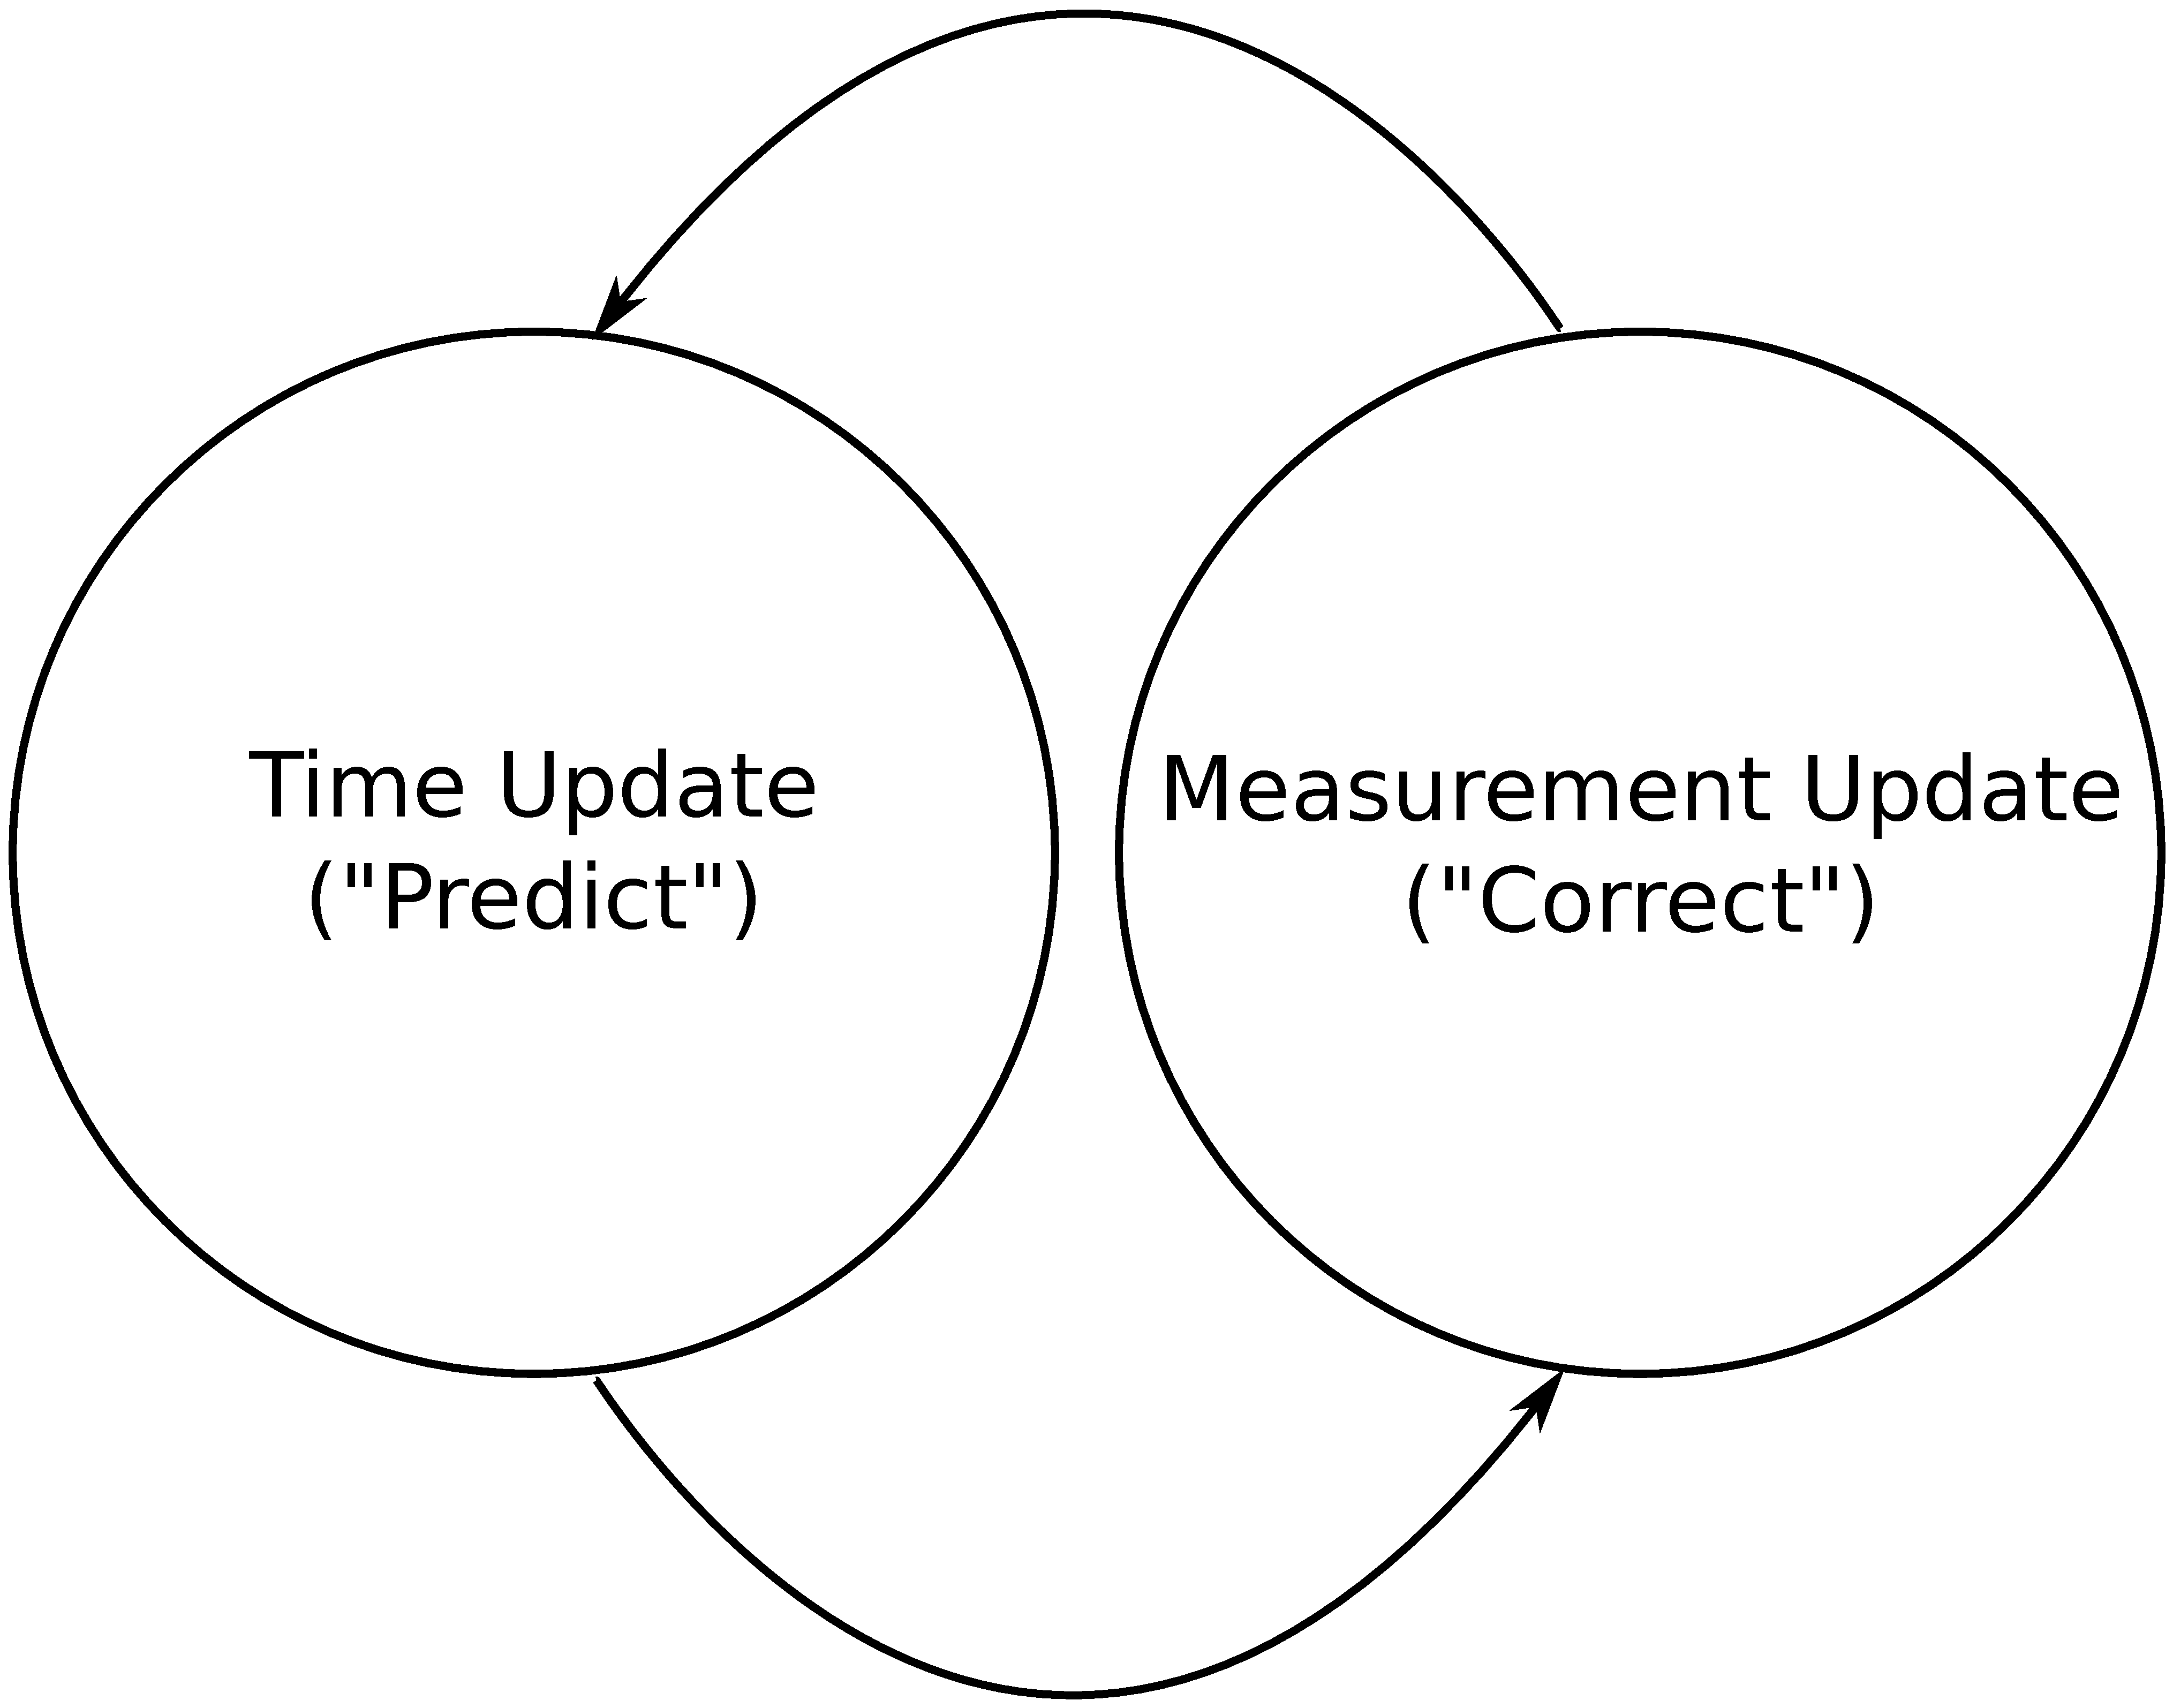
\includegraphics[width=0.5\linewidth]{kalman/fig/diagram-kalman.eps}
  \caption{Filtering process.}
\label{fig:diagram-kalman}
\end{figure}

One of its particularly useful features is the ability to combine together sensor measurements in mathematical form such that the solution is best possible estimate of the mean and the variance. 

Kalman filter uses three basic stages: prediction measurement and update. This would mean that the mean and the variance of the state are measureable. Prediction in case of moving vehicle is calculated based on previous vehicle location and dead reckoning.

Kalman gain determines the relationship between the importance of each previous estimation () and the current measurement (). Essentially - it expresses how much we trust in the measurement with respect to what we prediceted. According to the formula (), it is determined by matrices $Q$ and $R$ which represent process noise covariance and the measurement noise covariance (uncertainty), respectively. It takes values between 0 and 1 with 0 meaning that we use estimation only and give no importance to the measurement, and 1 that we consider direct measurement as the only important one.   

\section{Extended Kalman Filter (EKF)}

Real world models are rarely linear. The motiv for developing the Extended Kalman Filter is the adaptation of the linear Kalman Filter to dealing with nonlinear problems. However, it is possible that EKF significantly declines the performance quality \cite{julier96}. When making a prediction of state, observation or uncertainty of any of those for nonlinear systems, linearization can introduce errors. One example of such case is given in \cite{julier96}. The object follows the circular path. In such quite common case, the reason for failing in prediction is in linear approximations that EKF, by nature, uses when predicting the next state and its characteristics.

\section{Unscented Kalman Filter (UKF)}
Calculation-wise, the whole procedure is better than linearisation algorithm since there is no need for calculating the Jacobian, number of computations stays the same and it is easier to improvise with the algorithm by constraining or changing the samples \cite{julier96}.
\begin{algorithm}
\caption{UKF algorithm}
\label{alg:ukf}                   
%%%\begin{algorithmic}
%%%\INPUT state vector
%%%\OUTPUT feature vector \textit{fea}
%%%\FOR{$dist=0$ to $10$}
%%%\FORALL{$dir$ in \{0, 45, 90, 135\}}
%%%\STATE $glcm \leftarrow compute\ co-occurrence\ matrix\ for\ each\ pair\ of\ dist-dir$
%%%\STATE $normglcm \leftarrow normalize\ GLCM\ with\ the\ number\ of\ occurences$
%%%\STATE $harfea \leftarrow compute\ Haralick\ features$ \COMMENT{as in Appendix A}
%%%\STATE $fea \leftarrow [fea\ harfea]$ \COMMENT{store in feature vector}
%%%\ENDFOR
%%%\ENDFOR
%%%\end{algorithmic}
\end{algorithm}
\chapter{Navigation sensors} \label{chap:sensors}
This chapter gives an overview of the sensors used for localisation of an underwater vehicle and their characteristics. Underwater positioning can be based on usage of different types of sensors combined together in one system. The role of these sensors is to measure absolute position, velocities and heading/orientation. Localization is influenced with the development and performance of sensor devices. Sensors can be regarded as the means for managing the localization. Faster they are, more accurate they are, localization has more chances to perform better. Each sensor has its own reference system in which it operates. It is important to say that sensors output measurements with reference either in body frame (Figure ~\ref{fig:auv-axes}) - the one fixed to the object or in global frame (Figure ~\ref{fig:auv-positioning}). Basic navigation sensor set for a high-end AUV usually consists of depth sensor, magnetic compass, GPS device, LBL acoustic device, Doppler Velocity Log (DVL) and gyroscope, particularly fibre-optic gyroscope (FOG).   
\section{Inertial navigation system (INS)} \label{sec:ins}
Inertial navigation combines measurements of accelerometers and gyroscopes to track down the position and orientation of an object. Motion and rotation information obtained this way are processed in order to provide an estimate of objects location with respect to  initial reference. Recent INS configurations tend to consist of compact, more accurate and higher performance sensor devices.  
\subsection{Gyroscope}
Gyroscope is an INS sensor device that essentially measures orientation of the device. Although classic gyroscope measures orientation, modern gyroscopes are capable of measuring the angular rate. Gyroscopes can be mechanical, optical or MEMS gyroscopes. Underwater navigation uses fibre-optic gyroscope (FOG). FOG is based on measuring the interference of two light beams that pass through a coiled optical fibre in both directions. FOG provides quite precise information on rotation and its usage is intended for applications that demand higher performance. 
FOG can provide the angular information: rate of change of heading (yaw rate) and the yaw/heading itself. Both measurements can be used, depending on configuration. Since the sensor actually measures yaw rate (absolute measurement), yaw can be derived by integrating yaw rate in time. Disadvantage of such principally precise measurement, is that it is relative to previous yaw value and if that value turned out to be imprecise, drift can increase or contain a permanent bias. The KVH DSP-3000 device provides the Nessie vehicle with accurate angular rates.
\subsection{Doppler Velocity Log (DVL)}
DVL is intended to measure  velocities. Transceiver components mounted on the device, pointing downwards (towards the bottom) emit acoustic impulses which are expected to be reflected if the DVL is close enough to the bottom. In case of existing reflectance it is called having ``bottom-lock''. DVL usually has four transceivers. Each of them makes an angle with respect to the sea floor. If ``bottom-locked'', those four sensors undergo Doppler shift effect. Besides Doppler speeds, DVL measures roll, pitch and heading angles and fuses them together when computing surge, sway and heave velocity within the 3D speed vector in world referenced frame. The Teledyne Explorer PA DVL is used on Nessie AUV. This unit supplies the vehicle with altitude, surge, sway and heave velocities. Operation altitude ranges from 0.5 m to 80 m. Accuracy of the measured speeds is 0.7 cm/s when moving at the speed of 1 m/s.

\subsection{Magnetic compass} 
Magnetic compass provides 3D vector of local magnetic field. Magnetic compass points at magnetic north. Direction is determined so that it aligns with Earth's magnetic field. Important procedure before starting the compass usage is calibration. North direction as it appears on maps points to the geographic north (``true north''). That is the direction towards the rotation axis of the Earth. The direction of the \textit{magnetic north} does not overlap with the direction of the geographic north. Magnetic declination is an angle between magnetic north (measured by compass) direction and the true north direction (the one that maps refer to). Depending on location where the compass is used, magnetic declination can vary and the variation is different on different spots on the Earth's surface. Hence the calibration is necessary before usage. Magnetic compass gives measurements with slow variation in space. In addition, different magnetic effects caused by electric currents can affect the measurement, thus it is robust absolute measurement of heading, nonetheless, prone to noise. Nessie vehicle uses TCM 2.6 compass that precisely measures heading, pitch, and roll. Accuracy of the heading measurement is $0.8^{\circ}$.
\subsection{Depth sensor} 
Bathymetry system accomplishes depth measurement. It is possible to use the acoustic system for this purpose, however, bathymeter using pressure information tends to be more precise and trustable. Pressure sensor is standard piece of the equipment for an AUV. By measuring the pressure, it becomes possible to correlate the value of pressure with the value of depth. Device can frequently ascertain the absolute depth with good precision. A Keller Series 33X depth sensor measures the distance to surface having the depth range of 0 - 90 m and the accuracy of 0.05 m. 
\subsection{Global Positioning System (GPS)}
This well known satellite-based navigation system provides position information anywhere on the Earth surface or in the air, reasonably close to the surface. Due to absorption of electromagnetic waves in the water GPS signal is not available underwater. Despite the fact that GPS is not available, vehicles are equipped with GPS receiver intended to be used for initial position information before submerging or for occasional position updates if the vehicle temporarily goes back to the surface. Precision of the GPS position information can vary. Namely, range of the standard deviation errors can have the order of 25.27 m \cite{farrell98}. Such huge deviation can cause significant inaccuracies in navigation. An example of the influence of GPS imprecision was shown in Figure ~\ref{fig:with-gps}. Differential GPS (DGPS) \cite{farrell98} can be used in situations when better precision is needed.
\section{Acoustic positioning system}
Provides the absolute position, a ground-based reference. Principal way of exchanging the information through the environment is sound wave. Long baseline (LBL) is used for measuring position with respect to several tethered beacons with known position, placed in water (Section \S~\ref{sec:acoustic}). It can be understood as the extension of the GPS information below the water surface. Such system employs acoustic signals to measure the distances. Vehicle uses the acoustic transponder to send the acoustic wave (``pinging''). The wave reaches beacon and reflects back to the vehicle . LBL system consists of transceiver and array-arranged collection of beacons. LBL transceiver pings each of the beacons and detects the signal travel time in order to calculate the distance, knowing the speed of sound in water. Distances from the beacons are combined together in triangulation method. Triangulation makes it possible to determine the position of the robot in the network of fixed beacons. LBL position update can introduce the outliers that need to be rejected or filtered. 
%As stated in some practical implementations (\cite{blain03}), DVL and acoustic sensor perform ...
\begin{figure}
  \centering
    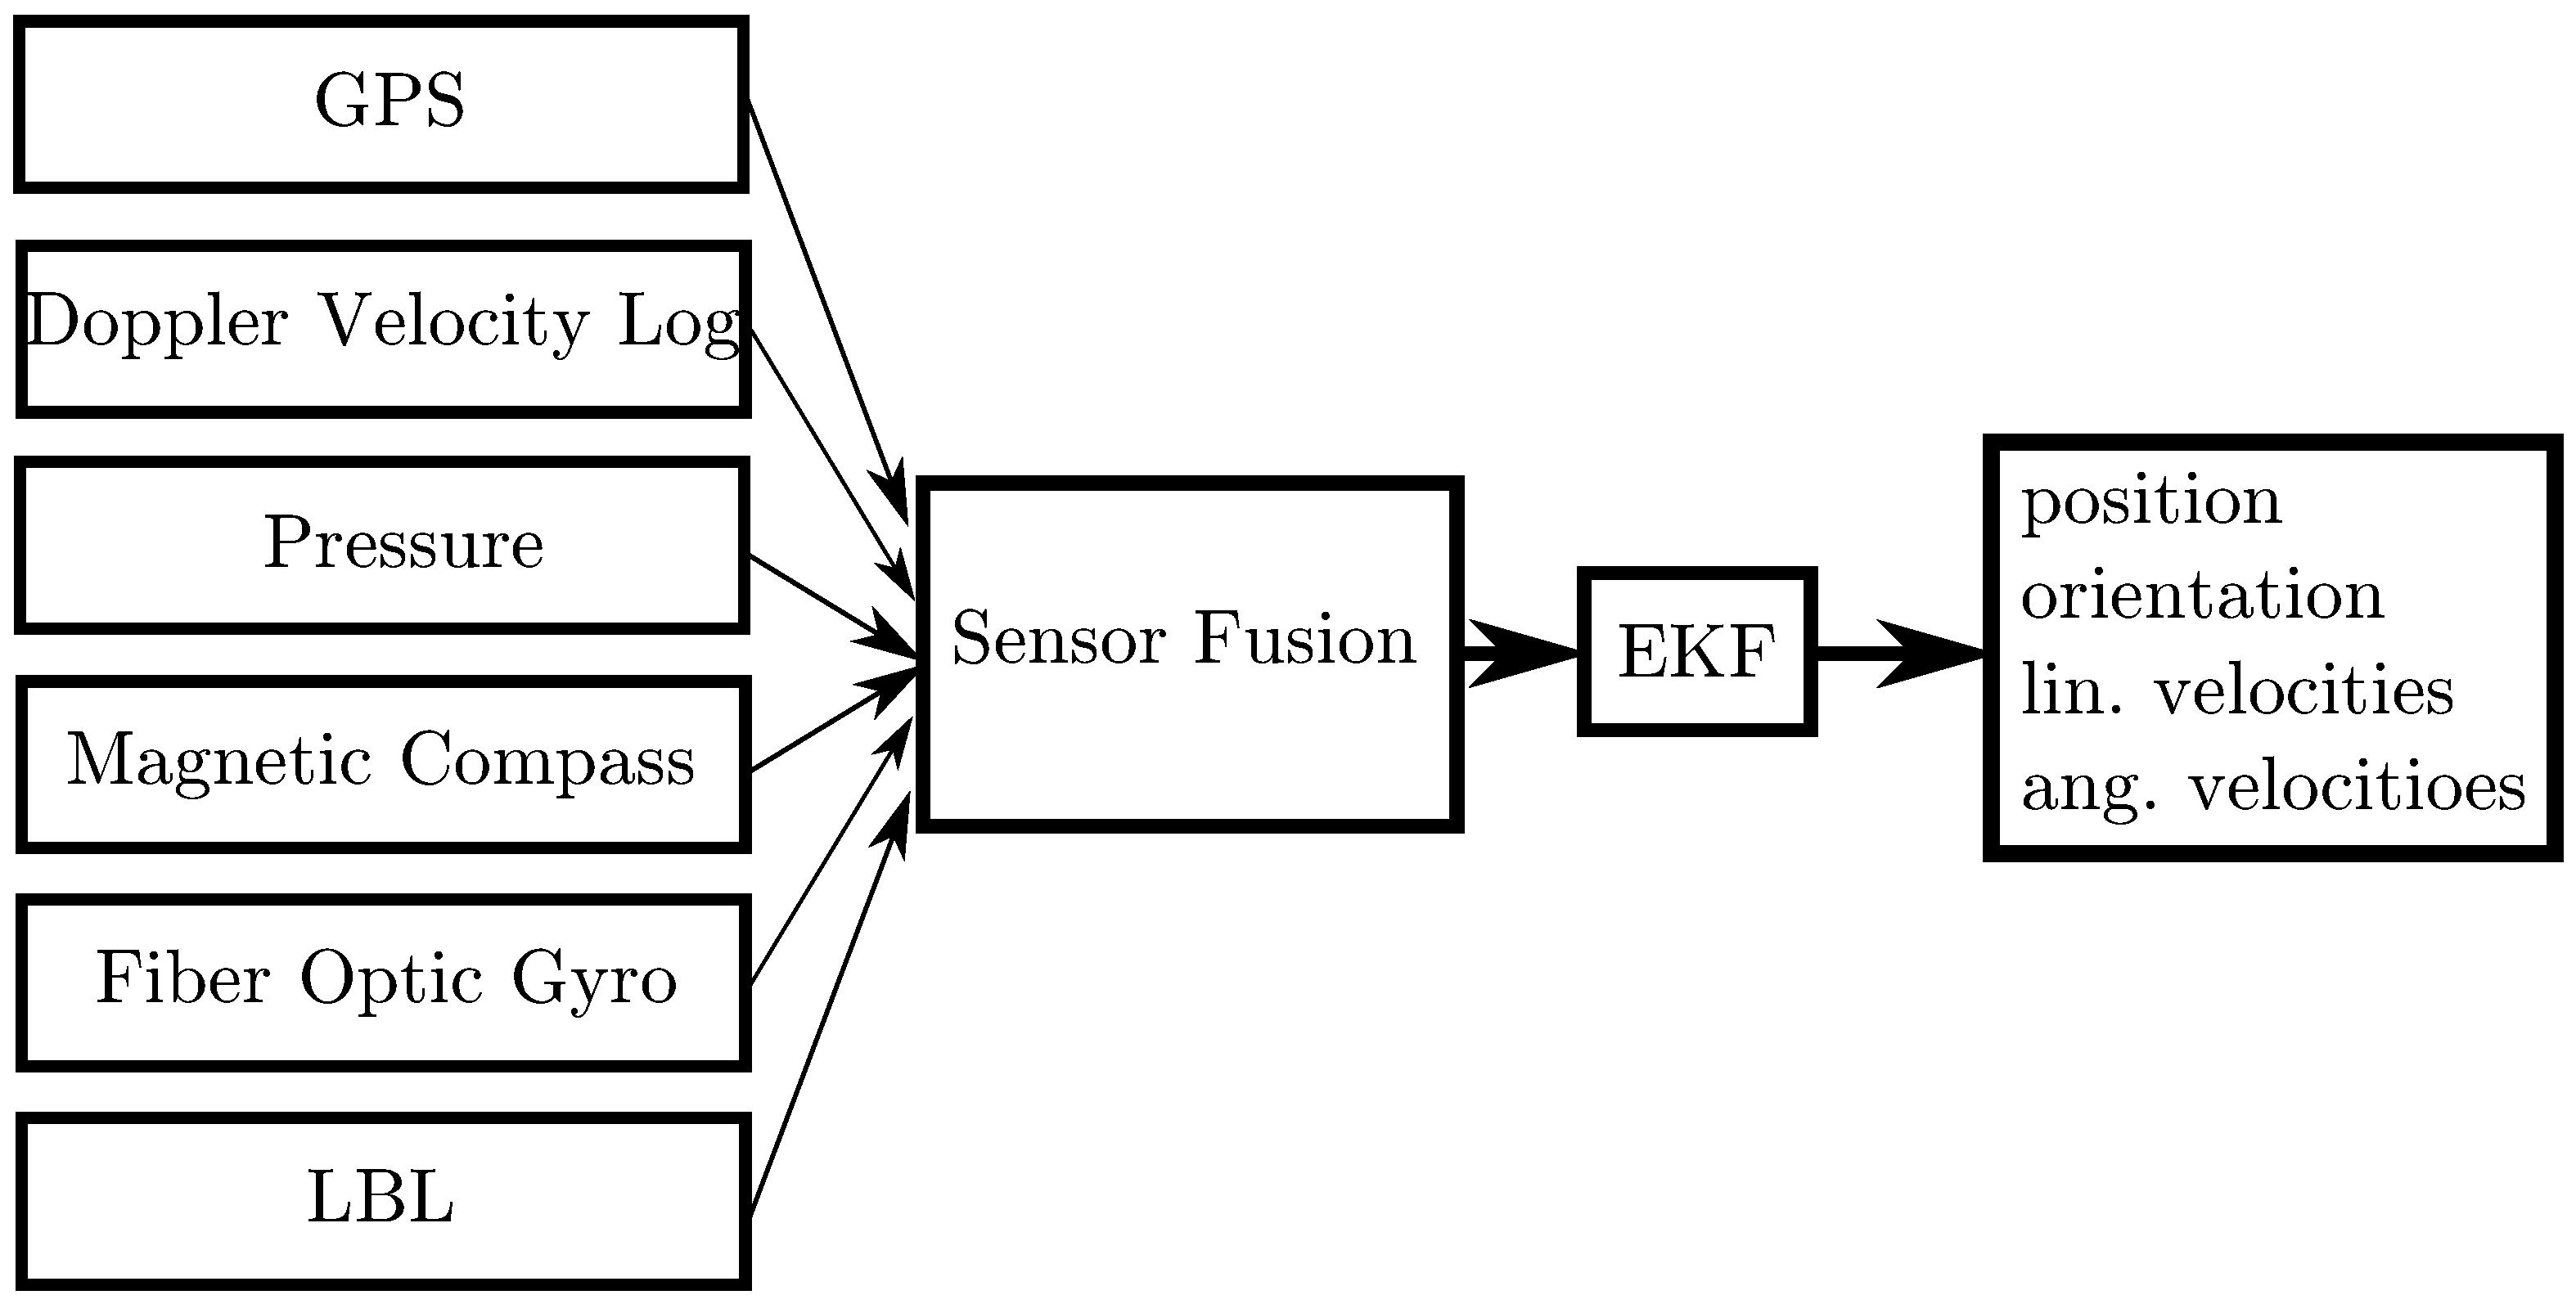
\includegraphics[width=0.65\textwidth]{methodology/fig/fusion.eps}
  \caption{Sensor fusion diagram.}
\vspace{-10pt}
\label{fig:sensor-fusion}
\end{figure}
\begin{table*}
\centering
	\caption{Navigation sensors characteristics.}
	\label{tab:sensors-char}
\begin{tabular}{llllll}
\toprule
Sensor      &     Measures     &   Update rate   &   Precision	  &    Accuracy    &    Range  \\
\midrule
\multirow{4}{*}{Pressure} & \multirow{2}{*}{depth} & \multirow{2}{*}{10 Hz} & 0.0002 $bar$ & 0.005 $bar$ & $0 - 10$ $bar$  \\
         	              &   &                         & (0.002 $m$)  &  (0.05 m)   & (0-90 $m$ in water) \\ 
                          & \multicolumn{5}{c}{\contra heave velocity is calculated by deriving depth in time - higher possibility of error} \\ 
        	              & \multicolumn{5}{c}{\pro distance from surface available no matter of distance from the seabed} \\                      
\midrule
\multirow{6}{*}{Compass}&yaw(heading)&\multirow{3}{*}{10 Hz}& $0.1^{\circ}$ & $0.8^{\circ}$ &              \\
         	            &pitch       &                       &               &               & tilt $\pm 50 ^{\circ}$  \\
         	            &roll        &                       &                &                &                    \\
  & \multicolumn{5}{c}{\pro absolute measure of heading - no drift } \\
  & \multicolumn{5}{c}{\contra needs magnetic north correction (due to magnetic declination)} \\
  & \multicolumn{5}{c}{\contra prone to magnetic disturbance} \\
\midrule
\multirow{2}{*}{FOG} & \multirow{2}{*}{yaw rate} & \multirow{2}{*}{5Hz} & \multirow{2}{*}{$ < 1^{\circ} / hr$} & \multirow{2}{*}{$\pm 20^{\circ} / hr$} & \multirow{2}{*}{$\pm 375 ^{\circ}/s$} \\
     &          &           &           &         &         \\
 & \multicolumn{5}{c}{\pro high accuracy in heading measurement, compared to compass} \\
 & \multicolumn{5}{c}{\contra drifts over time, needs correction for the Earth rotation} \\
\midrule
\multirow{3}{*}{DVL} & surge velocity & \multirow{3}{*}{10 Hz} & \multirow{3}{*}{$0.1\frac{cm}{s}$} & $ \pm 0.7\frac{cm}{s}$ at $1\frac{m}{s^{4}}$ & \multirow{3}{*}{$\pm 9.5\frac{m}{s}$} \\
         	        &sway velocity&                        &                                    & $ \pm 1.9\frac{cm}{s}$ at $3\frac{m}{s^{4}}$ &                                  \\
         	        &heave velocity &                      &                                    & $ \pm 3.0\frac{cm}{s}$ at $5\frac{m}{s^{4}}$ &                              \\
 & \multicolumn{5}{c}{\contra relative measurement of velocity} \\
 & \multicolumn{5}{c}{\contra requires depth - looses lock at $0.6$ $m$ altitude resulting in no output} \\
\bottomrule
\end{tabular} 
\end{table*}
\chapter{Navigation capabilities of AUVs} \label{chap:capabilities}
This chapter gives an overview of the main navigation elements for an underwater vehicle. Methods and existing algorithms for underwater vehicle localisation have been summarized. Section \S~\ref{sec:lit-review}  gives an overview of the literature and related work reporting various AUV navigation methods. 

Carrying out underwater vehicle localisation implies using concepts such as \textit{vehicle state} within the \textit{navigation strategy} framework. Those two concepts will serve as a starting point for reviewing different methods. It is possible to refer to the definition of the vehicle state and its features when categorizing navigation solutions. On the other hand, navigation solutions can be essentially based on different ideas (strategies). In addition, we could treat any kind of localisation as absolute or relative, depending on which reference system we use when obtaining measurements. Absolute localisation takes environment point as reference system while relative considers the vehicle itself to be the reference. Most of the techniques surveyed here deal with absolute localisation. 
\section{State estimation}
Vehicle navigation state describes its position within the environment. The state is a vector that contains variables relevant for localizing the vehicle. State interpretation would further categorize navigation methods on those that treat state as stochastic: linear or nonlinear, or deterministic \cite{kinsey06}. Thus, navigation state estimators can be based on stochastic state estimators or deterministic state observers \cite{kinsey06}.
% which introduces some special features
%For an underwater vehicle, localization is accomplished using unbiased estimation such as Extended Kalman Filter (EKF). 
\section{Stochastic state estimators}
The name of stochastic state estimation methods suggests that states are treated as ultimately having feature of randomness built-in. That means being or having a random variable, or grouping random values in certain manner. It does not seem to be a wrong conclusion after recognizing that state of a system, is seldom known precisely. It is the essential nature of the process or the instrument used for measuring or the estimation algorithm itself that it fails at submitting utterly accurate data all the time. We could say that many natural phenomena are random with certain distribution of the randomness. Random variable distributions are conveniently treated as Gaussians. Statistically speaking, estimation is a rule used to calculate an estimate of a variable of interest using the observed data. As it is the case with random variables, we can say that certain state has an expected value, and that such ``randomness'' can be expressed with the distribution formula, resulting in descriptor values such as mean and standard deviation that fully describe the distribution in particular case of Gaussian, for instance. This approach has been applied often in underwater navigation. Most notable stochastic state estimator is Kalman filter (Section \S~\ref{sec:kf}). Kalman filter is an unbiased, optimal estimator \cite{kalman60, grewal01}. KF works through iterations by employing the process model for making the state prediction and the observations for doing the state correction (Figure ~\ref{fig:diagram-kalman}). Kalman filter and the Extended Kalman Filter (EKF) treat random variable as having a Gaussian distribution. Sections \S~\ref{sec:kf} and \S~\ref{sec:ekf} provide more details on Kalman filtering. A number of works report on usage of different variations of Kalman filters for state estimation. %Following paragraphs make an overview of various stochastic estimator usage with the objective of determining (estimating) values that represent system state - location of the robot in the environment. Methods considered for this review exploit different sensor types.
%However, it is not the only component. 
\subsection{Linear stochastic state estimators}
Localisation of a robot naturally requires sensor measurements. Methodologies that work with state estimation employ measurements in terms of adding them as supplementary information to the mathematical model of object movement. Linear kinematic models are not suitable for describing the dynamics of the vehicle, therefore most of the solutions implement nonlinear stochastic state estimation.   
%within Kalman filters was introduced in chapter on filtering, \S~\ref{chap:kalman}
%where the whole procedure involves
\subsection{Nonlinear stochastic state estimators}
The necessity of linearising the plant and observation models to comply with linear Kalman Filter is the basis of EKF derivation. Various works report the usage of other interesting nonlinear estimators such as Unscented Kalman Filters (UKF). Methods that are based on random sampling (``Monte Carlo methods''), for instance Particle Filters (PF), are also used for localization underwater, which brings us back to the concept of stochastic value, but from the perspective of sampling those stochastic values. The work presented in the thesis focuses on nonlinear stochastic state estimators such as EKF and UKF.
%\section{Nonlinear filtering} 
%(such as defining underwater vehicle location) 
\T{Nonlinearity } is a common phenomenon. Real world consists of various nonlinear systems. Practical situations often demand the usage of approximations that eventually lead to linearisation. The solution obtained this way is claimed to be sub-optimal - not perfectly tuned, but, indeed, useful. The problem is to consecutively make an estimation of the state of a dynamic system using a sequence of noisy measurements \cite{ristic04}. State-space approach turns out to be suitable choice when dealing with nonlinearity and estimating (filtering) values of the group of variables. Number of filters have been designed to deal with the phenomenon. Depending on the methodology, they could be roughly categorized as \cite{ristic04}: 
\begin{itemize}
\item those that use analytic approximations (e.g. EKF)
\item those that use numerical approximations
\item those that use multiple models
\item those that use sampling (e.g. UKF)
\end{itemize} 
Since approximations eventually lead to linearising the system, a short overview of linear Kalman Filter (KF) is given in order to make an introduction on something that will be the basis for methods presented.
\section{Kalman Filter (KF)} \label{sec:kf} 
KF \cite{kalman60}  is a well known mathematical tool that offers solution to \textit{linear-quadratic problem} in form of an estimator \cite{grewal01,ristic04}. Such linear estimator is optimal in terms of any quadratic function of the estimation error \cite{grewal01}. It is based on an iterative and recursive process. In addition, it is well suited framework for blending together different sensor measurements. Mathematically speaking - world consists of variety of systems that change their state $(\vect{x}(k))$ in time. Guided by this foundation, science has established a concept of \textit{linear dynamic system model} (Table ~\ref{tab:system}) consisted of \textit{process model} and \textit{measurement model}. \textit{Process model} (Table ~\ref{tab:system}) is perturbed by Gaussian white noise $(\vect{n})$. It emulates the behaviour of a phenomenon (change of the states) together with its hereditary randomness. \textit{Measurement model} (Table ~\ref{tab:system}) emulates observations of the system state. Observations are expressed as linear functions of state variables corrupted with Gaussian white measurement noise $(\vect{m})$, similarly as the process model itself. System can receive control inputs $(\vect{u}(k))$. Covariances of the process $(\vect{n})$ and measurement $(\vect{m})$ noise, are $\vect{Q}$ and $\vect{R}$ respectfully. Covariances are important components of filtering algorithm ~\ref{alg:kf}. They can be interpreted as uncertainties in particular prediction or measurement.
\begin{table*}
\centering
	\caption{Overview of the state-system models.}
	\label{tab:system}
\begin{tabular}{cc}
\toprule
\multicolumn{2}{c}{System models overview} \\
\multicolumn{2}{c}{$\vect{x}$ - system state vector, $\vect{u}$ - control input, $\vect{n}$ - process noise, $\vect{m}$ - measurement noise} \\
\midrule
\multirow{1}{*}{Linear System Model}  &  \multirow{1}{*}{Nonlinear System Model} \\
\multicolumn{2}{c}{process model:} \\
\multirow{2}{*}{$\vect{x}(k) = \vect{A}\vect{x}(k-1)+\vect{B}\vect{u}(k)+\vect{n}(k-1)$} 
									& \multirow{2}{*}{$\vect{x}(k) = f(\vect{x}(k-1),\vect{u}(k),\vect{n}(k-1))$} \\ \\
\multicolumn{2}{c}{measurement model:} \\
\multirow{2}{*}{$\vect{z}(k) = \vect{H}\vect{x}(k)+\vect{m}(k)$} 
									& \multirow{2}{*}{$\vect{z}(k) = h(\vect{x}(k),\vect{m}(k))$} \\ \\
\bottomrule
$\vect{A}$ matrix associates $(\vect{x}(k-1))$ and $(\vect{x}(k))$ & $f()$ nonlinear process function \\
$\vect{B}$ matrix associates $(\vect{u}(k-1))$ and $(\vect{x}(k))$ & $h()$ nonlinear measurement function \\
$\vect{H}$ matrix associates $(\vect{x}(k))$   and $(\vect{z}(k))$ &   \\
\\
\multicolumn{2}{c}{$E\lbrace \vect{n}(k) \rbrace = E\lbrace \vect{m}(k) \rbrace = 0$} \\ 
\multicolumn{2}{c}{$E\lbrace \vect{n}(k) \vect{n}(j)^{T} \rbrace =  \delta_{kj} \vect{Q}, E\lbrace \vect{m}(k) \vect{m}(j)^{T} \rbrace = \delta_{kj} \vect{R}$} 
\end{tabular} 
\end{table*}

The Discrete Kalman Filter is an optimal unbiased minimum mean squared error estimator. It is a calculation process that works recursively, passing iterations as shown in diagram ~\ref{fig:diagram-kalman}. Kalman filter uses three basic steps: prediction, measurement and update. One iteration uses process equation, next one proceeds further using prediction result within the observation equation. Recursion continues each time referring to previous filter output.

Assumptions that KF uses:
\begin{itemize}
\item distribution of a random variable is assumed to be Gaussian, therefore mean and variance can fully describe it
\item linear transform of a Gaussian distribution gives another Gaussian distribution 
\end{itemize}
In spirit of that, noise vectors ($\vect{n}, \vect{m}$)  and thus linearly derived state and observation vectors ($\vect{x}, \vect{z}$) are Gaussian. Another assumption is that noise vectors $n$, $m$ have zero mean values (``white Gaussian'') and that their elements are not correlated, resulting in diagonal matrices $\vect{Q}$ and $\vect{R}$ (Table ~\ref{tab:system}).

%\begin{wrapfigure}{r}{0.5\textwidth}
%\vspace{-10pt}
\begin{figure}
  \centering
    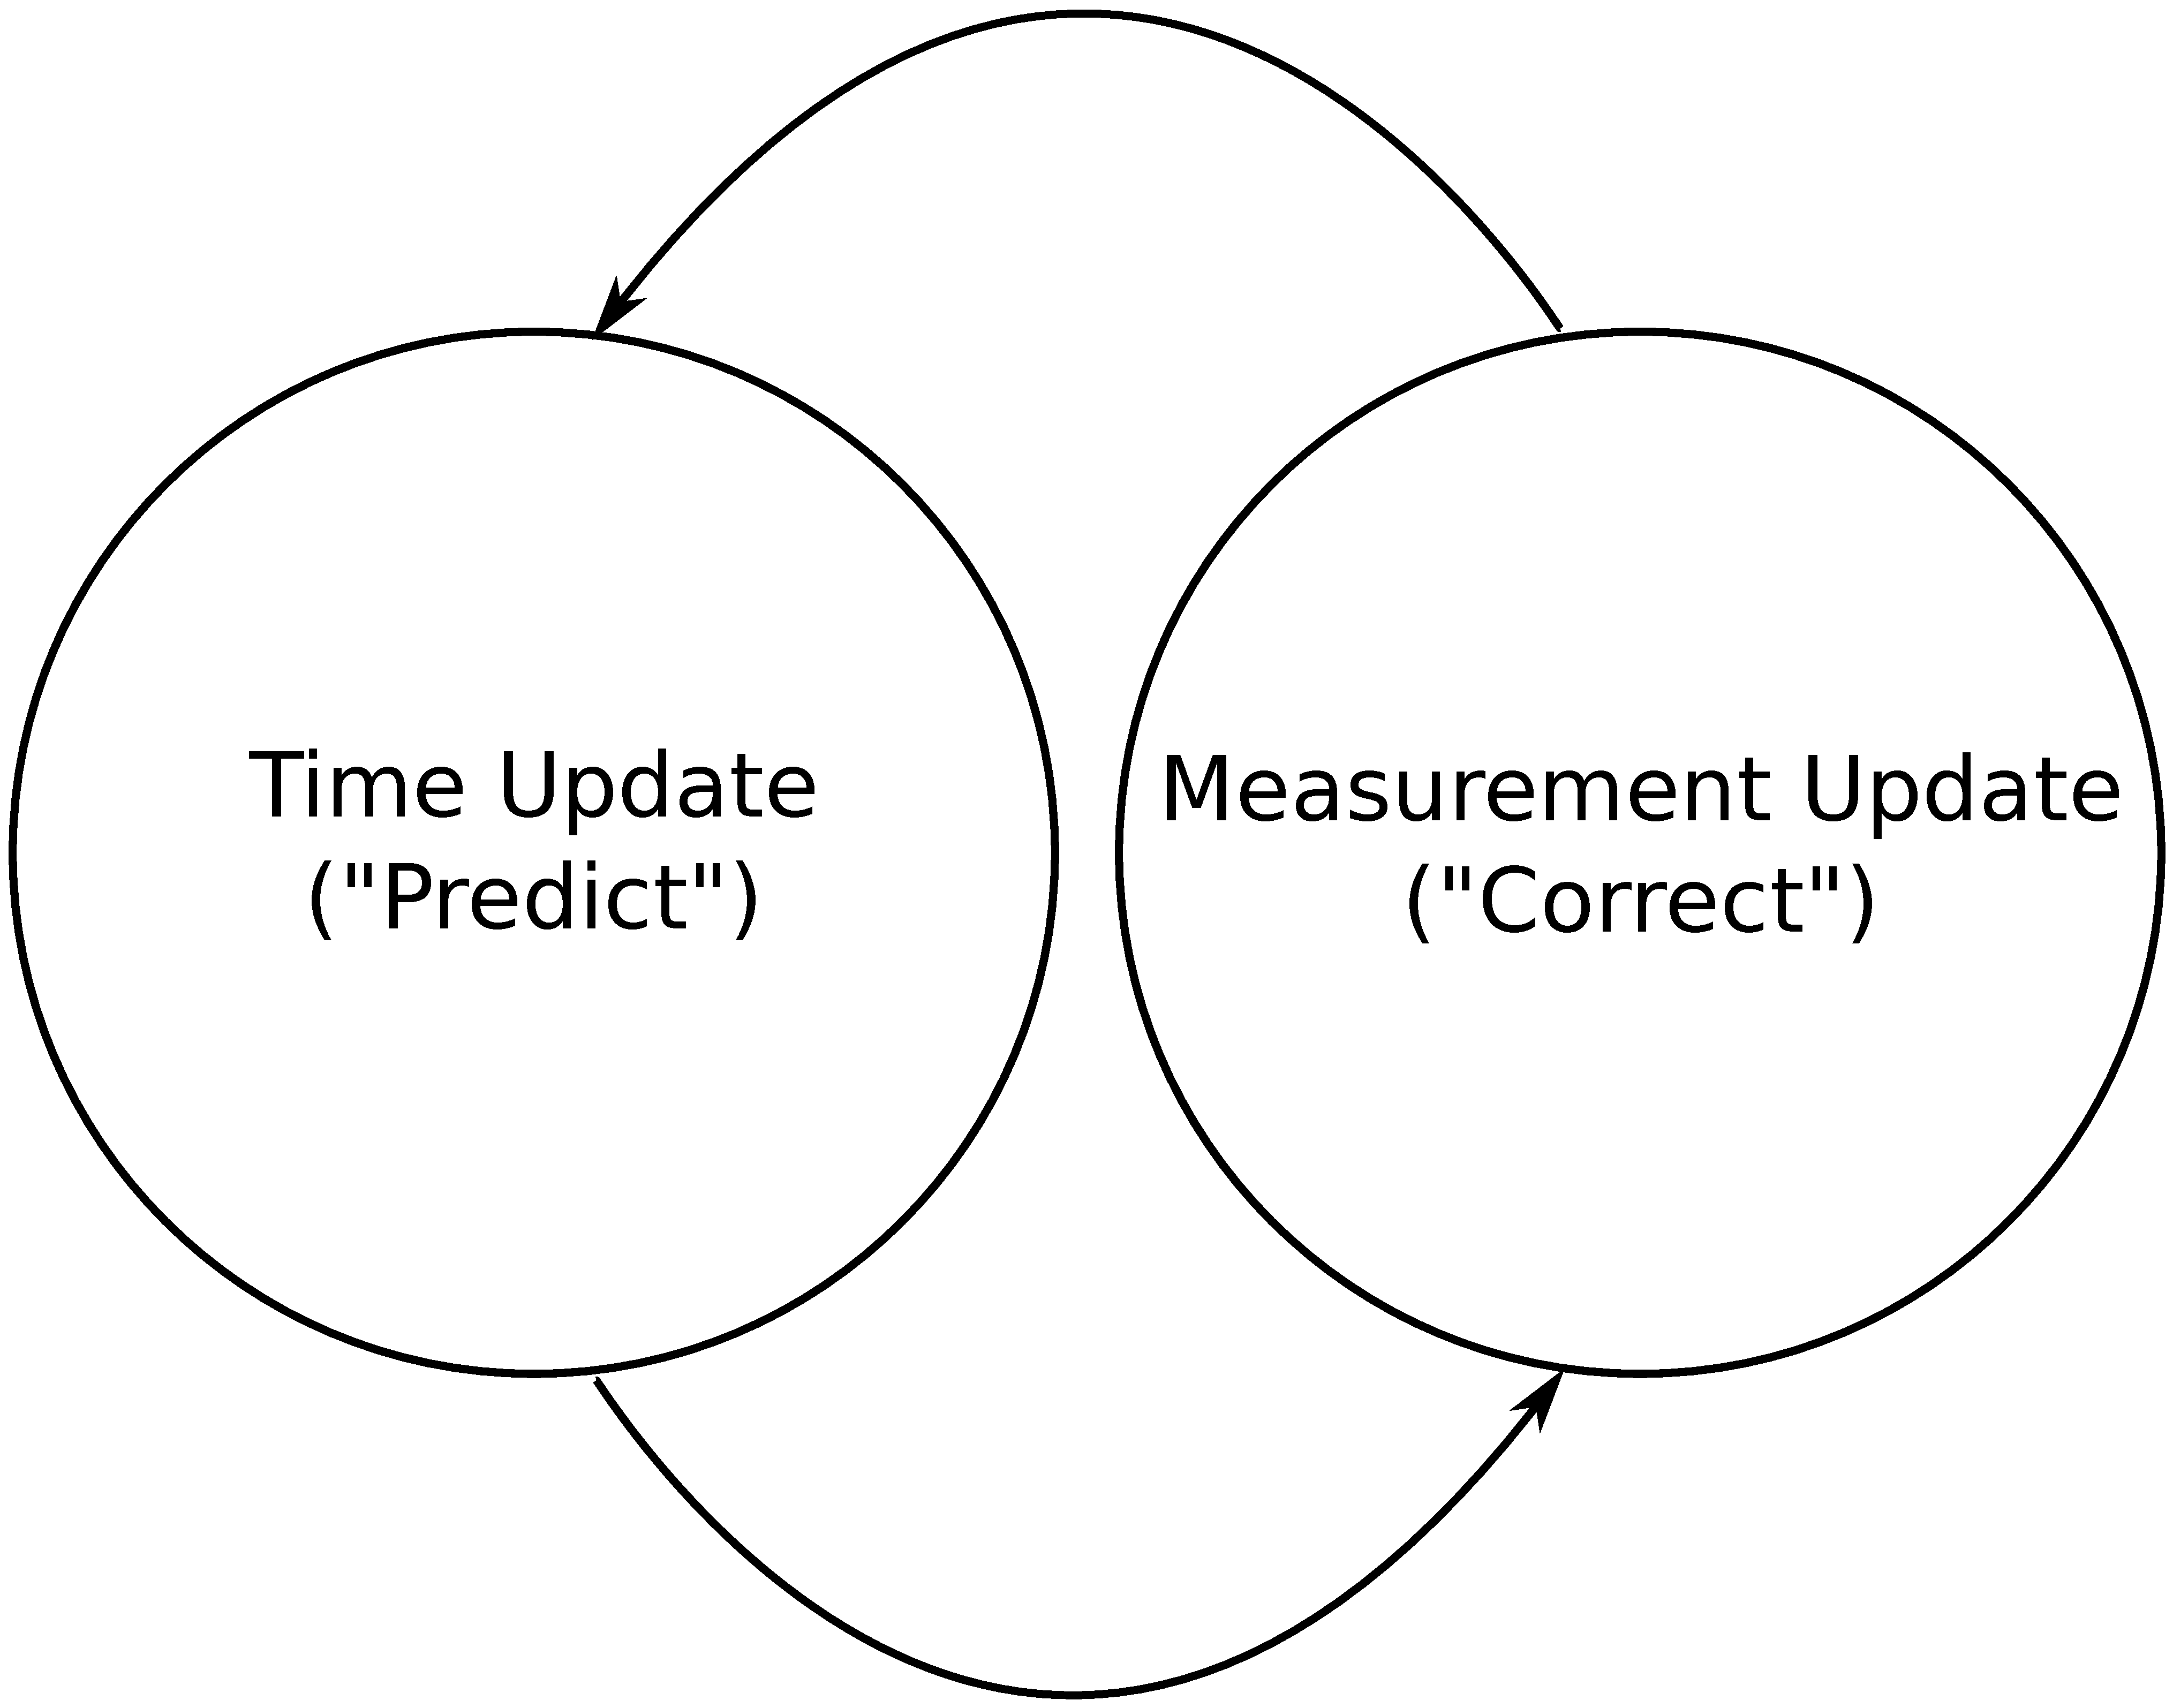
\includegraphics[width=0.4\textwidth]{kalman/fig/diagram-kalman.eps}
  \caption{Filtering process.}
\vspace{-10pt}
\label{fig:diagram-kalman}
\end{figure}
%\end{wrapfigure}

KF can be summarized with the set of formulas given in Algorithm ~\ref{alg:kf}. The aim of the equations is to recursively obtain the estimate of the state vector ${\vect{\hat{x}}}$ and the uncertainty of such estimate. Uncertainty is described as state variance $\vect{P}(k) = E\lbrace (\vect{x}(k) - \vect{\hat{x}}(k)) (\vect{x}(k) - \vect{\hat{x}}(k))^{T} \rbrace$. KF defines states as collection of elements with Gaussian distribution, thus mean value is used as an estimate and variance as a measure of how far the values are spread out around mean. Notation follows the one from the Table ~\ref{tab:system}. $\vect{\hat{x}}(k \mid l)$ is a state estimate at the time $k$ using observations obtained until time moment $m$. It is a recursive estimator since every estimation relies on previous state estimation and current observation (measurement). Although history of previous observations is not directly used, it is still incorporated in previous state estimation. Previous state estimation is used in current state estimate due to recursive nature of the algorithm. Transformation uncertainty $\vect{Q}$ is updated simultaneously with the state. Innovation $\nu$ presents difference between the real observation and predicted observation. Both innovation and its covariance matrix $\vect{S}$ are included in calculation of Kalman gain $K$. Kalman gain does the final state estimate correction ~\ref{alg:kf} influenced by recent observation and makes the uncertainty optimal with respect to quadratic estimation error criteria.
%Depending on case, incorporating the  uncertainty  or the noise uncertainty $\vect{R}$.
\begin{algorithm}%[h!]
\caption{The Discrete Kalman Filter} \label{alg:kf}
\begin{algorithmic}
\REQUIRE $E\lbrace \vect{x}(0) \rbrace = \vect{x}(0) = \vect{\hat{x}}(0)$
\COMMENT{initialize state}
\REQUIRE $\vect{P}(0) = \delta_{jk} \vect{P_{0}} $ 
\COMMENT {initialize covariance}
\LOOP 
	\STATE $k \Leftarrow k+1$ 
	\STATE $\vect{\hat{x}}(k \mid k-1) = \vect{A} \vect{\hat{x}}(k-1) + \vect{B} \vect{u}(k)$
	\COMMENT {state prediction}
	\STATE $\vect{P}(k \mid k-1) = \vect{A} \vect{P}(k-1) \vect{A}^{T} + \vect{Q}$
	\COMMENT {state prediction uncertainty}	
	
	\STATE $\nu = \vect{z}(k) - \vect{H} \vect{\hat{x}}(k \mid k-1)$	
	\COMMENT {innovation}
	\STATE $\vect{S} = \vect{H} \vect{P}(k \mid k-1) \vect{H}^{T} + \vect{R}$	
	\COMMENT {innovation uncertainty}	
	\STATE $\vect{K} = \vect{P}(k \mid k-1) \vect{H}^{T} \vect{S}^{-1}$	
	\COMMENT {``Kalman gain''}	
	
	\STATE $\vect{\hat{x}}(k) = \vect{\hat{x}}(k \mid k-1) + \vect{K} \nu$
	\COMMENT {state correction} 
	\STATE $\vect{P}(k) = (\vect{I}-\vect{K}\vect{H})\vect{P}(k \mid k-1)$
	\COMMENT {state correction uncertainty}
	\RETURN $\vect{\hat{x}}(k), \vect{P}(k)$
\ENDLOOP
\end{algorithmic}
\end{algorithm}
Although essentially intended for dealing with linear system, KF formulas are be important starting point in understanding nonlinear filtering accomplished with Extended Kalman Filter (EKF) or Unscented Kalman Filter (UKF).

\section{Deterministic state estimators}
Deterministic state estimators refer to non-stochastic system (plant, process) and observation (measurement) model. Stochastic means that the input and output can manifest in some random behaviour. Concept of deterministic state does not imply any uncertainty. However the estimation, apart from being precise and accurate, can be characterized with its stability. Estimation is exact (no randomisation of the variables) and estimator should be asymptotically stable \cite{kinsey07}. Stability is defined using different mathematical criteria \cite{kinsey07}. In this case, navigation elements such as speed or position or even full-state vector are an output of some defined transfer function. In order to know the transfer function, an estimator of the nonlinear transfer function model is used. Such approach utilizes the exact knowledge of nonlinear dynamics of the vehicle. Essentially, estimating deterministic state implies passing the input data through a certain transfer function so that the outputs are localisation related values. Transfer function is defined using known formulas of the transfer function and parameters which are estimated by giving particular input and observing the corresponding output of the system in order to recognize its behaviour. Being a completely different concept, in terms of methodology  they are not the focus of the thesis.
%Deterministic state estimators have not been extensively used in AUV localisation.
\section{Strategy} 
Now that the state vector is revealed as a storage for describing the vehicle location, finding a way to filter that state vector - stochastic or deterministic, linear or nonlinear, can employ different approaches. At this level, we can talk about the strategy - general approach, an idea. The primary navigation system in most of the applications, including underwater navigation, is Inertial Navigation System (INS) (Section \S~\ref{sec:ins}). Since such system accumulates noisy data, it introduces the drift errors that need to be occasionally corrected inside the navigation algorithm. Various ways of correcting those errors were developed. Most widely known ``correction tool'' is the incorporation of an absolute position measurement. Numerous literature that considers integrating occasional GPS or LBL measurement within the stochastic state estimation algorithm is presented in Section ~\ref{sec:lit-review}. 
%It usually manifests as some form of the GPS information adopted to be used underwater.
Oceanographic community typically uses three different strategies to handle the absolute positioning underwater \cite{whitcomb99}: (1) transponder networks on the seafloor (long baseline, LBL), (2) ship-AUV communication (short baseline), and (3) sensors mounted on the underwater vehicle that measure range and inertial motion. They can be combined together depending on the idea, purpose or conditions. Each of the strategies is different in terms of accuracy, costs, complexity \cite{eustice05} or types of sensors used. Section \S~\ref{chap:sensors} gives more insight into performance and categorization of each inertial sensor device used for underwater vehicle navigation. Naturally, most of the conventional methods rely on acoustic waves used for measuring the distance. Nevertheless, visual information is used, especially in transparent or structured environment \cite{carreras03}. Navigation can be combined with simultaneous localization and mapping approach (SLAM, Section \S~\ref{sec:slam}), or can be terrain aided (Section \S~\ref{sec:terrain-aided}) \cite{kinsey06}. Although not common for many applications, visual information recorded by the camera or a pair of cameras can be used to aid navigation (reduce the drift) \cite{eustice05large, bahr08}. If the localization involves control of the vehicle movement coupled with localisation and environment information, then it is addressed as active localisation. On top of already mentioned methods, some novel strategies in which vehicles communicate among themselves, such as cooperation for navigation (Section \S~\ref{sec:cooperation}), are explored \cite{bahr08}. Following chapter gives an overview of the mentioned strategies.       

\section{Acoustic-based localization techniques} \label{sec:acoustic}
In the absence of possibility to transmit radio waves, acoustic communication emerges as solution for communication underwater. Considering that the electromagnetic waves are absorbed and the propagation of light is limited, positioning cannot rely on GPS signal, laser scanners, visually aided navigation, or radio communication. Therefore, state of the art in absolute positioning of the robot underwater implies triangulation using distances from navigation buoys positioned at the known locations (Figure ~\ref{fig:gib-lbl}). Alternative solution is to surface back in order to update the position using GPS. 
 
Underwater acoustic positioning system is the main tool used to track underwater vehicles. Reason for relying on acoustics is the nature of the water environment:resistant to radio waves, leaving out mechanical acoustic disturbance as the only mean of communication. Three classes of underwater acoustic positioning systems are used (Figure ~\ref{fig:lbl}): Long Baseline (LBL), Ultra Short Baseline Systems (USBL), Short Baseline Systems (SBL) and GPS intelligent buoys (GIB). 

LBL systems (figure ~\ref{fig:standard-lbl}) use a network of two or more sea-floor mounted (anchored) baseline transponders to reference the navigation. Such system is considered to be accurate, generally with accuracy better that 1 meter - usually around few centimetres \cite{noaa01}. However, communication-wise, such system is convenient for small number of vehicles, since one vehicle can query the network each time \cite{bahr08}. Hence, having a large number of vehicles can cause delays in update. Elapsed time between moment of sending the query and receiving the response is used to estimate the time-of-flight ($t_{flight}$) of the wave and eventually the distance ($d$) between beacon and the vehicle, considering that the speed of the sound ($c$) is known and the essential relation $c = \frac{d}{t_{flight}}$ is used for calculation. By using methods such as triangulation, these distances can be used to compute the AUV's absolute position. LBL systems can be long-range or short-range. Long-range systems use 12 kHz frequencies for communication range of 10 km of distance with the error varying from 1 up to 10 m \cite{whitcomb99combined, bahr08}. Short-range systems use 300 kHz frequencies and operate within the range of 100 m with sub-centimetre precision \cite{whitcomb99combined, bahr08}. 
 
SBL systems (figure ~\ref{fig:short-lbl}) do not require sea-floor mounted transponders. Instead SBL system uses a vessel equipped with high-frequency directional emitter in order to accurately determine the AUV position with respect to the vessel \cite{maurelli08}. Disadvantage of such system is the need for providing a vessel and the distance limits since the range between the ship and the AUV has to be short. Moreover, SBL accuracy improves with transducer spacing (possibility of longer baseline). Similarly, the range measurements are used to triangulate the position. Transducer sends a signal, transponder located on the vehicle responds yielding distance information. AUV's location is determined with respect to transducers' location.

USBL systems (figure ~\ref{fig:ultra-short-lbl}) uses similar beacons as LBL system. Difference is that vehicle has transceiver with several receiving elements positioned close to each other on a known distance so that the reply from beacons is detected by all of them. It is possible to calculate the phase difference between received signals this way which is enough to determine the bearing to the beacon. If the distance information is combined together with bearing, then the absolute position of the vehicle can be estimated just by considering the response of only one beacon. 

GIB systems (figure ~\ref{fig:gib-lbl}) consist of floating buoys supplied by GPS signal carrying transducers. Vehicle has a transponder that replies to transducer query with acoustic signal, enabling buoys to register the time-of-flight. Such concept communicates opposite way from the one accomplished in standard LBL.    

\begin{figure}%[htp]
  \begin{center}
    \subfigure[Standard LBL]   {\label{fig:standard-lbl}   
    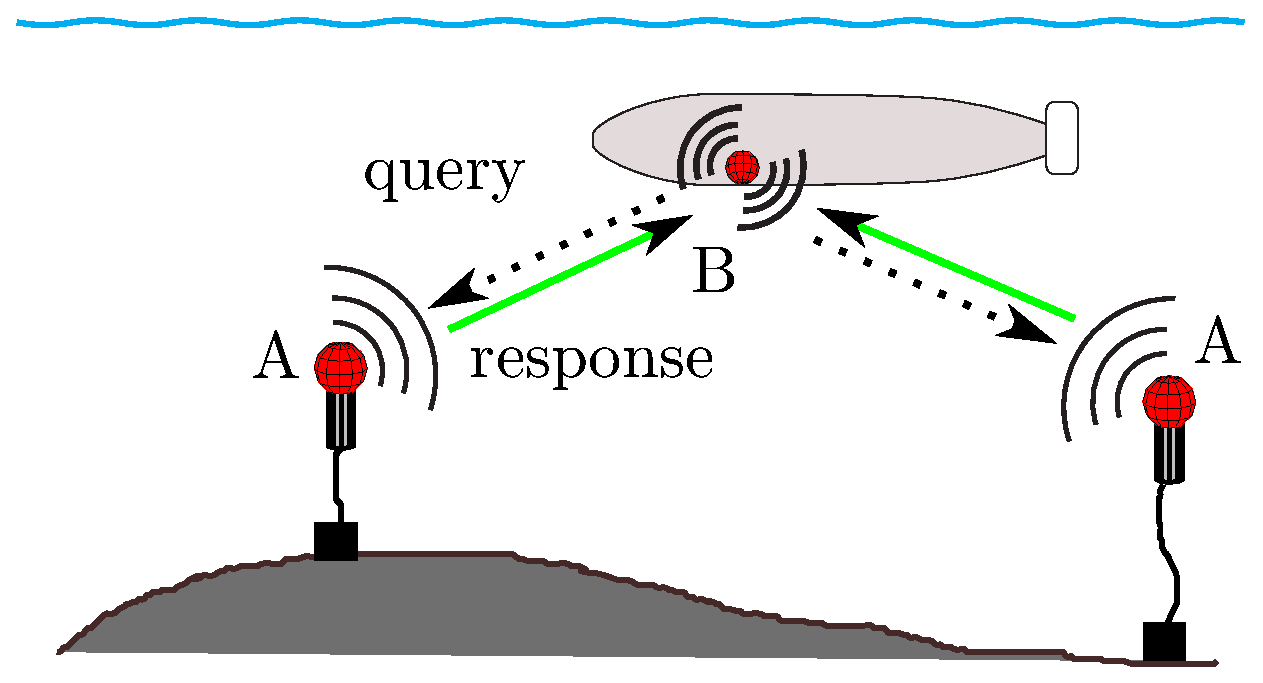
\includegraphics[width=0.45\textwidth]{auv-overview/fig/standard-lbl.eps}}
    \subfigure[Ultra-short LBL]{\label{fig:ultra-short-lbl}
    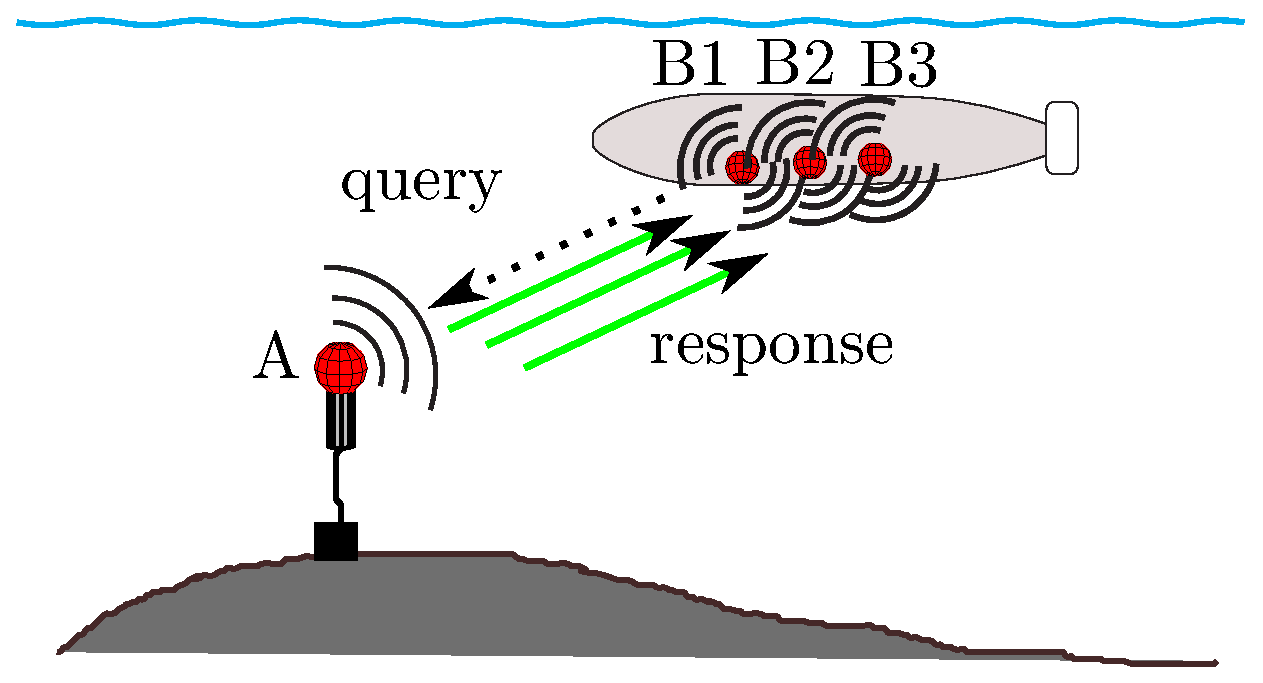
\includegraphics[width=0.45\textwidth]{auv-overview/fig/ultra-short-lbl.eps}}   \\
    \subfigure[Short LBL]      {\label{fig:short-lbl}      
    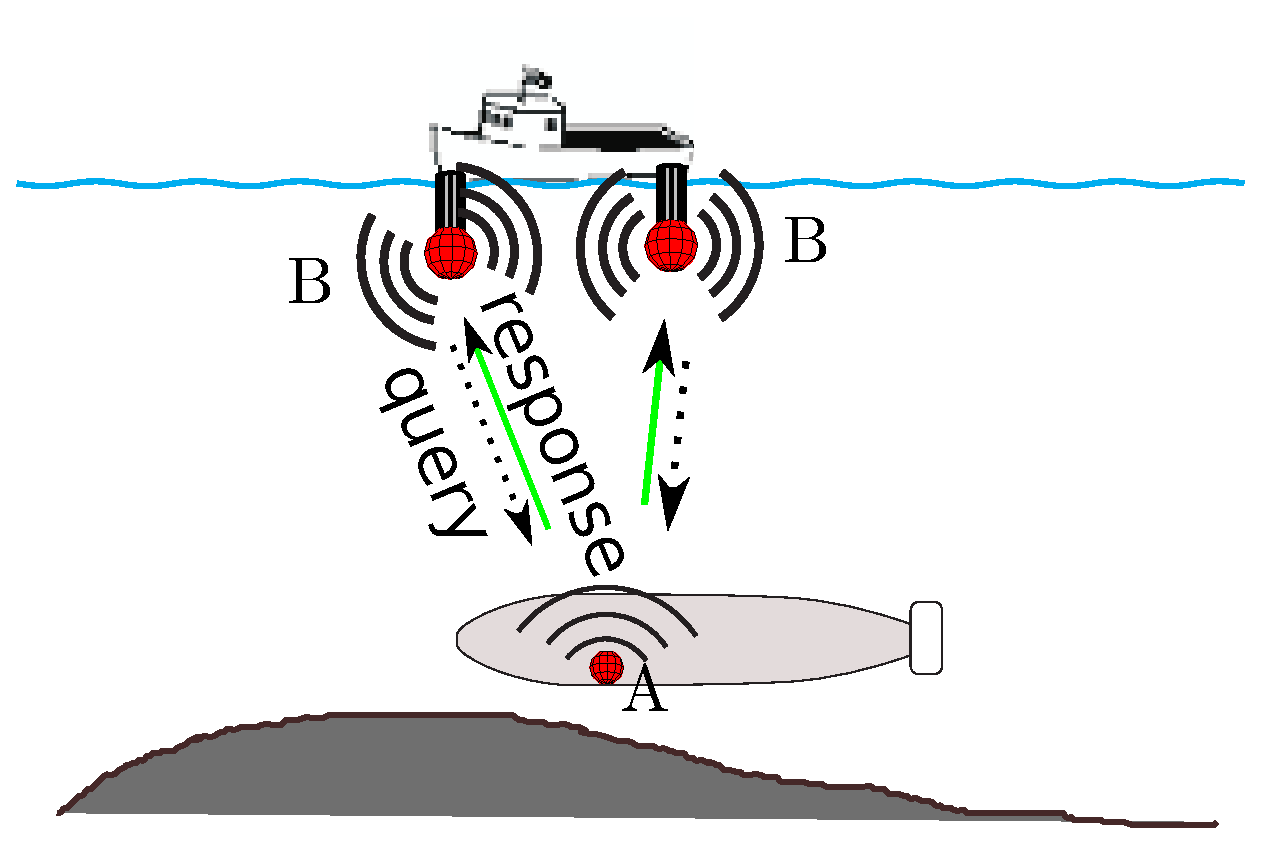
\includegraphics[width=0.45\textwidth]{auv-overview/fig/short-lbl.eps}} 
    \subfigure[GPS intelligent buoys]  {\label{fig:gib-lbl}      
    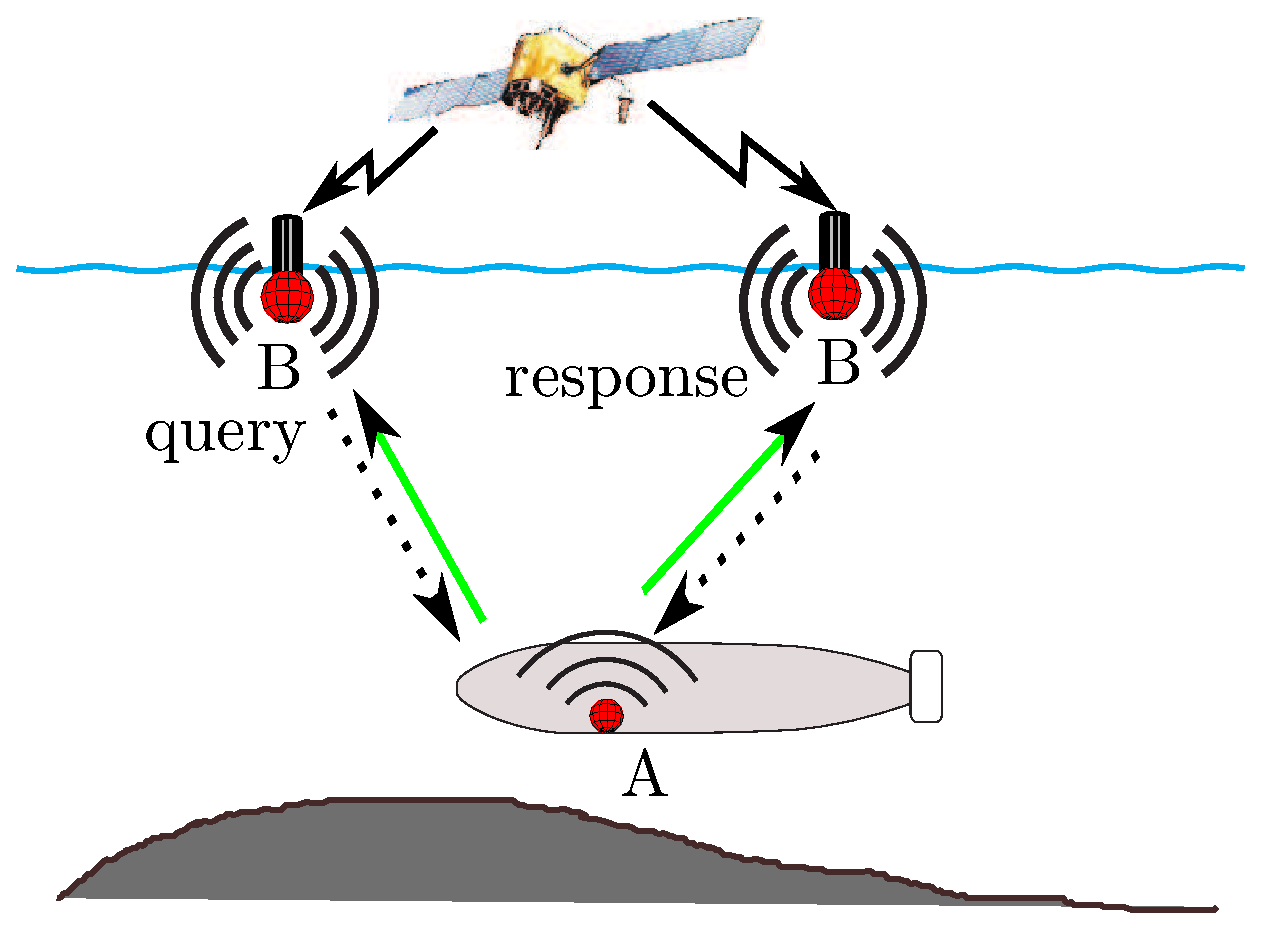
\includegraphics[width=0.45\textwidth]{auv-overview/fig/gib-lbl.eps}}
  \end{center}
  \caption{Different variants of LBL: A - transponder, B - transducer.}
  \vspace{-10pt}
  \label{fig:lbl}
\end{figure}
Common feature for all the mentioned systems is that the position is inferred from the acoustic feedback of transponders so that the vehicle is capable of locating itself with respect to transponders. Outliers and noise are 

\section{Terrain-aided navigation} \label{sec:terrain-aided}
Terrain-aided navigation can be used to determine the vehicle position using topographic, magnetic or gravitational data \cite{kinsey06}. Terrain-aided navigation can rely on the map of the sea bottom, its elevation or some particular landmarks that are detected to fix the vehicle position. In such circumstances, it is possible to define the map first and try to navigate with respect to that map (map known a-priori) or manage the mapping and navigation simultaneously using sensor data to build the map from the scratch, step by step. Disadvantage of terrain based methods lies in fact that they depend on precision of the map of the floor and ability of the vehicle to sense the depth or image the sea floor. In most of navigation scenarios, a-priori maps are not available \cite{kinsey06}.
The essential sensor for terrain aided navigation is sonar that measures the distance (``time-of-flight''). However it is possible to use the optical sensor devices, for instance cameras, and process the visual information. Range of optical sensors is much shorter, they usually require structured environment, fairly good visibility within the water and the optical information cannot spread as freely and as far as the acoustic information does. However, its nature of information is different, richer with different types of data, including the raw position data. 
\section{SLAM} \label{sec:slam}
Concentrates on establishing essentially autonomous navigation algorithm that would be environment based. Therefore, it is reducing the need for additional infrastructure and using the spatial information from environment to bound the position error. Idea of the concept called SLAM is to localize the robot with respect to environment landmarks \cite{ruiz01}. To accomplish that, two challenging tasks have to be solved: extracting the features and finding a way to measure correspondence between measurement and the feature. Literature offers some solutions to SLAM based approach. Brief overview of some of the methods is given in Section \S~\ref{sec:lit-review}. 
\section{Cooperation for navigation} \label{sec:cooperation}
Advancement in acoustic modems has made it possible to establish more reliable communication and develop communication technologies that engage data from more than one vehicle \cite{bahr08, fallon10}. Idea of involving number of vehicles in exploration is to consider sensor and state information sent from the other vehicles. Advantage of this approach is reduction in amount of sensor equipment, for instance LBL transponders or bathymetry sonars. However, more vehicles need to be deployed. 
\section{Active localisation} \label{sec:active-nav}
Active localisation integrates together control of the robot motion and localisation algorithm. Active refers to vehicle ``activity'', mobility or movement since these strategies sense the environment and combine together localisation with control so that the quality of the localisation is improved. Idea is to guide the motion of the vehicle in order to make it more convenient for the localisation algorithm to work out the tracking \cite{petillot10}.
\section{Related work on AUV navigation}\label{sec:lit-review}
Following paragraphs summarize the documented ways to process the sensor information in order to be able to estimate the position within the environment. 

In existing survey on underwater vehicle navigation, Kingsey \cite{kinsey06} gives a summary presenting the methods used for navigation. As introduced in \cite{kinsey06}, current vehicle position is referred as navigation state - a vector whose elements express where the vehicle is and how it is oriented in space with respect to some reference. Localization simply means finding a way to estimate navigation state vector. Naturally, sensors are providing the data for the estimation.

The simplest approach would be dead reckoning - to take the raw sensor measurements and use them directly or within a simple mathematical model that describes the vehicle dynamics. Instead, many techniques presented in literature utilize sensor data as supplementary information together with the information from the kinematic model.

Underwater navigation is using several instrumentation methods to carry out the robot localization in the sea \cite{whitcomb99}. These include transponder networks placed on the bottom of the sea, tracking systems between the ship and the underwater vehicle, and sensory devices that measure range and dynamics mounted on the vehicle itself. Each of the methods has its advantages and disadvantages. Transponder network gives accurate position information, however using it requires installing and calibrating additional equipment \cite{eustice05}.

\subsection{Kalman filtering localisation}
Some past works have already dealt with the issue of managing robot localization using Kalman filtering. Master thesis of Negneborn \cite{negenborn03} gives a useful overview of the theoretical knowledge in field of probability and estimation. Thesis also surveys the utilization of Kalman filtering for localizing vehicles in general. Emphasis is on application in robotics. Several experiments have been reported in the thesis with a detailed discussion. This work is a good starting point in learning and understanding the problem of localization on physical robots in general and, in particular, usage of Kalman filtering for that purpose.

Blain et al. \cite{blain03} study the application of Kalman filter in navigation of an underwater vehicle used for water dam inspection focusing on merging position orientation and velocity information. This algorithm uses acoustic positioning sensor together with the integration the DVL sensor (Chapter \S~\ref{chap:sensors}) measured velocities \cite{blain03} to estimate the position. Apart from reporting performance of \textit{sensor-fusion} in real application, several issues have been pointed out and dealt with in their work, such as managing asynchronous information that arrives from sensors. It is reported that Kalman filter output could be corrupted in situations when observations (sensor measurements) are subject to interruption or periodic stopping. Due to the fact that not all the sensors can be always available, it is usually necessary to be capable of adding or removing sensor observations from the system without changing the navigation algorithm. 

Asynchronous data delivery in this particular case means that the DVL sensor (Chapter \S~\ref{chap:sensors}) provides data with higher rate \cite{blain03}. Such obstacle was solved by switching to estimation procedure so that it is suitable for that particular sensor measurement scenario. This simply means that if the acoustic sensor and DVL sensor asynchronously provide new measurements, Kalman filtering is used to carry out the fusion by doing filter switching process. Each sensor has a filter process attached to it and the sensor itself defines which filter becomes active for the actual measurements. Otherwise, pure DVL velocity measurement is just integrated to update the position, as dynamic model would suggest.  
% (take into account both measurements at the correction stage).
Blain also analyses delays in absolute position measurement and validity of absolute position data if they are delayed. This effect evident in case of acoustic waves, where the real time of the measurement is current measurement time minus the time it took for the acoustic signal to arrive. It is especially visible in cases when acoustic signal moves across a longer distance. This causes a delay in data arrival. To overcome this, position estimate between two acoustic measurements is memorized. Position is meanwhile normally updated by integrating the DVL data that happen more frequently. To compensate for the time it took for the acoustic signal to arrive, timestamp of the moment when the data was produced was estimated and memorized together with the current position at the timestamp. The procedure consists of two stages: at first, a new position estimate is made using the recieved acoustic position data to update the position at the timestamp. Finally, the correction is applied on the updated position by integrating velocities that happened in meanwhile - from the timestamp till the actual time. This serves as the correction of the position estimate error influenced by significant time of flight of the signal. 

Drolet et al. \cite{drolet00} introduce a flexible localization strategy based on sensor fusion and usage of several Kalman filters arranged together in a bank. Each filter is reduced to express a simple kinetic equation. In addition, each filter processes one state - works in one ``dimension''. Idea is to integrate together sensor measurements that arrive at different time moments from different sensors. Method takes asynchronous information from sensors, manages a filter switching process so that the most recent data is used to update those filters that can be updated with such measurement \cite{drolet00}. Such sensor fusion strategy is adaptable in terms of number of sensors so that the best is taken out from the available input data, more robust to data loss. Moreover, asynchronous inputs are allowed. 

Di Massa et al. report usage of Kalman filter framework for slightly different concept of navigation that takes surrounding terrain as reference for estimating the position of the sonar (``terrain-relative navigation''), \cite{diMassa97}. In their work, sonar image is matched to the map using mean absolute difference (MAD) as the matching criterion. Matching map location is considered as the measurement of the vehicle position \cite{diMassa97}. Matching process is not entirely transparent - there are always several candidates eligible to be candidate for best matching. Thus several matchings are selected and weighted depending on how much they relate to the terrain images. Weights correspond to uncertainties in estimation theory. Quality of similarity is used to weight each measurement. Solution consists of having resulting best estimate of location \cite{diMassa97}. Information from selected matches is combined to make the best estimate. The role of Kalman filter framework is to carry out the estimation. Each of the chosen matches is considered as one measurement together with its weight as uncertainty. The filtered state is the position of the image within the map. 

Gade and Jalving introduce post processing aided navigation system deployed on a commercial underwater vehicle \cite{gade99}. Idea is that the underwater vehicle records sensor data while accomplishing mission under the sea surface (capturing images of the seabed). At the same time, a vessel is positioned on the surface receiving information of its position through the reliable Differential Global Positioning System (DGPS). After the mission is over, data are combined together with position data that was simultaneously recorded on the survey vessel located on the surface. Kalman filtering is used when merging the data. \textit{Error-state} Kalman filter \cite{gade99} is used to combine sensor measurements and their error models. Observations in case of such filter consist of the difference between measured and computed values. Instead of working directly with states, presented algorithm filters the errors, so that the ultimate position and heading estimate can be derived by subtracting the estimated errors from, as authors suggest, corresponding calculated state elements. This way, final aim of obtaining more accurate vehicle position and heading together with the tunable accuracy of such estimate \cite{gade99} contibutes in improving the accuracy of obtained seabed maps. 

Dissertation \cite{roman05} suggests how to improve the vehicle position estimation when reconstructing maps of the sea floor. Visual information of the terrain is used as the feedback that makes terrain mapping data and the vehicle navigation data more consistent. Inspiration for investigating lies in fact that map-making depends on localization quality. Navigation errors are potentially large scale particularly seriously affecting the results when mapping is vehicle-based \cite{roman05}. Existing local navigation is used together with terrain-relative measurements. Namely, terrain sub-maps are created over short periods while the vehicle works out the inaccurate localization using dead reckoning. Sub-maps are registered resulting in position measurements between two vehicle states, placing an additional constraint on the vehicle position estimates. Delayed EKF is used to merge together the measurements (``sub-map'' registrations and previously reached vehicle locations) into the navigation framework. Delayed state version of the recursive EKF enables retaining knowledge of prior platform positions.  

Yun et al. introduce simulation and present testing results of the navigation system that combines the usage of Inertial Measurement Unit (IMU) together with GPS fixes that occur less frequent and asynchronously \cite{yun00}. Asynchronous Kalman filter with six states for orientation and eight states for position estimation is implemented \cite{yun00}. Process model takes the velocities and GPS bias, models them as white noises passed through the first order systems with the time constant. Measurement consists of synchronous (periodical) velocity measurements and asynchronous DGPS information. The design of the filter for the position estimation algorithm conforms to the standard routine, with the difference that the measurement vector has different length depending on the number of available valid sensor inputs, hence it has a flexible size, but each observation updates the state vector of the fixed size \cite{yun00}. The idea of the asynchronism enables that DGPS signals are used, if available and as soon as they are available, together with the speed measurements. This way, the localization algorithm uses the most of the data that are currently available.

The usage of the stochastic estimators implies using a known model that describes system state transition from one moment to another (\textit{plant model}) and model that describes transition from state to the measurement (\textit{observation model}). Such model does not have to be the same each time. Jakuba and Yoerger \cite{jakuba03} study the way to optimize navigation by estimating the vehicle model parameters, for instance various dynamics or buoyancy coefficients that normally influence the model, but are treated as constant. Their study involves post-processing of the navigation data and heuristic estimate of these coefficients' optimal value. Real missions that applied the technique resulted in reduced noise in localization data, therefore giving clearer tracking. 

Julier and Uhlmann introduce the method that carries out nonlinear filtering \cite{julier96}. It is an alternative generalization of the KF that changes the approach of representing mean and variance of the random variable after it passes through an nonlinear transform. Their research is a quite useful and comprehensive theoretical overview of filtering in general and the role of Extended Kalman Filter (EKF) in switching to nonlinearity world. Introduced filter, later known as Unscented Kalman Filter (UKF) is regarded as more precise alternative to EKF that is, in addition, fairly easy for implementation. Julier and Uhlmann in their work point out the shortcomings of the EKF. In search of general method that would overcome the problem, instead of using proposed equations for projecting mean and covariance, a discrete set of points is chosen and projected using a chosen non-linear transformation (Section \S~\ref{sec:ukf}). Idea is to use the parameters to approximate the Gaussian distribution instead of approximating the nonlinear transformation. This way, propagation of the information is accomplished directly, and the aim is to find a way to parametrise the information about the mean and covariance of the distribution. Advantages of the filtering algorithm are in terms of precision and simplicity (no need for Jacobian derivation) with empirical results for highly nonlinear problems including vehicle control indicating as good as or better performance than EKF and higher robustness.

Wan and van der Merwe \cite{wan00} go further in exploring the concept of UKF introduced by \cite{julier96}. Their research briefly reminds of disadvantages manifested in EKF and improvements gained with the usage of UKF. UKF theoretical backgrounds, the idea itself and meaning of used variables were explained in comprehensive manner in one of the document sections. Usage of UKF was reported together with the results in different estimation problems such as nonlinear system identification, state estimation, parameter estimation and dual estimation problems \cite{wan00}. UKF according to the authors achieved higher accuracy compared with EKF in all the domains that were examined.

At this point, it is useful to make a short digression in order to give more details on EKF and UKF.

\subsubsection{Extended Kalman Filter} \label{sec:ekf}
System can be described with set of states that evolve in time according to mathematical functions that are nonlinear in many applications. Table ~\ref{tab:system} gives an overview, categorizing systems as linear or nonlinear. Nonlinear state prediction would use previous state estimate and mean value of the process noise:
\begin{equation}
\vect{\hat{x}}(k \mid k-1) = f(\vect{\hat{x}}(k-1), \vect{u}(k), 0)
\label{eq:state-pred-nonlin}
\end{equation} 
EKF is intended for solving sub-optimal state estimation of a nonlinear system. The main characteristic of EKF is that it analytically approximates - linearises - the process and measurement functions ($f()$ and $h()$, Table ~\ref{tab:system}). Linearisation implies approximating these functions with their first derivative around current prediction, similarly as the ordinary functions are approximated with Taylor polynomials of first degree. In this case, derivation is slightly more complex since model functions $f()$ and $h()$ take several input vectors and output the resulting vector. Hence, the derivation will consist of partial derivation of process per state input vector (Equation ~\ref{eq:der-proc-state}) and per noise input vector (Equation ~\ref{eq:der-proc-noise}). And partial derivation of measurement function per state (Equation ~\ref{eq:der-mes-state}) and measurement noise (Equation ~\ref{eq:der-mes-noise}). Partial derivatives themselves will be Jacobian matrices considering that vector is derived per vector. 
\begin{equation}
\vect{F}(k) = \frac{\partial f}{\partial x} (\vect{\hat{x}}(k \mid k-1), \vect{u}(k), 0)
\label{eq:der-proc-state}
\end{equation} 
\begin{equation}
\vect{W}(k) = \frac{\partial f}{\partial n} (\vect{\hat{x}}(k \mid k-1), \vect{u}(k), 0)
\label{eq:der-proc-noise}
\end{equation}
\begin{equation}
\vect{H}(k) = \frac{\partial h}{\partial x} (\vect{\hat{x}}(k \mid k-1), 0)
\label{eq:der-mes-state}
\end{equation} 
\begin{equation}
\vect{V}(k) = \frac{\partial h}{\partial m} (\vect{\hat{x}}(k \mid k-1), 0)
\label{eq:der-mes-noise}
\end{equation}
Subsequently, filtering process can be treated similarly as classic, discrete linear Kalman filter introduced in previous section. 
\begin{algorithm}%[h!]
\caption{The Discrete Extended Kalman Filter} \label{alg:ekf}
\begin{algorithmic}
\REQUIRE $E\lbrace \vect{x}(0) \rbrace = \vect{x}(0) = \vect{\hat{x}}(0)$
\COMMENT{initialize state}
\REQUIRE $\vect{P}(0) = \delta_{jk} \vect{P_{0}} $ 
\COMMENT {initialize covariance}
\LOOP 
	\STATE $k \Leftarrow k+1$ 
	\STATE $\vect{\hat{x}}(k \mid k-1) = f(\vect{\hat{x}}(k-1), \vect{u}(k), 0)$
	\COMMENT {state prediction}
	\STATE $\vect{P}(k \mid k-1) = \vect{F}(k) \vect{P}(k-1) \vect{F}^{T}(k) + \vect{W}(k) \vect{Q} \vect{W}^{T}(k)$
	\COMMENT {state prediction uncertainty}	
	
	\STATE $\nu = \vect{z}(k) - h(\vect{\hat{x}}(k \mid k-1), 0)$	
	\COMMENT {innovation}
	\STATE $\vect{S} = \vect{H}(k) \vect{P}(k \mid k-1) \vect{H}^{T}(k) + \vect{V}(k) \vect{R} \vect{V}^{T}(k)$	
	\COMMENT {innovation uncertainty}	
	\STATE $\vect{K} = \vect{P}(k \mid k-1) \vect{H}^{T}(k) \vect{S}^{-1}$	
	\COMMENT {``Kalman gain''}	
	
	\STATE $\vect{\hat{x}}(k) = \vect{\hat{x}}(k \mid k-1) + \vect{K} \nu$
	\COMMENT {state correction} 
	\STATE $\vect{P}(k) = (\vect{I}-\vect{K}\vect{H}(k))\vect{P}(k \mid k-1)$
	\COMMENT {state correction uncertainty}
	\RETURN $\vect{\hat{x}}(k), \vect{P}(k)$
\ENDLOOP
\end{algorithmic}
\end{algorithm}
Process model mathematically describes how the state changes for the given input (Equation ~\ref{eq:state-pred-nonlin}). Essential invention in EKF algorithm is the linearisation of the given function around current state mean and variance which further results in estimation process similar to the one described for linear Kalman filter.
%There can be various number of states and all of them are grouped together in the state vector. Navigation system could, for instance, group together position coordinates and orientation angles in the state vector. If the system is considered as discrete, transition from one discrete value of the state vector to the next one, is described with the function $f$ called process model, equation ~\ref{eq:state-transition}, where the current state, $x(k+1)$, is calculated using the process model with previous state ($x(k)$), current input ($u(k+1)$) and process noise ($v(k+1)$) as arguments. In other words, 
%Thus, our system is not entirely an unknown black box once a linear Kalman Filter(KF) is attached to it. A hint about its dynamics is known in form of process model. The only information available once the filtering starts, are its control inputs ($u$) and a set of observations ($z$). equation associates observations with the state. Similarly as shown in ~\ref{eq:state-transition}, $x$ and $u$ present the state, while $w$ represents the additive measurment noise and function $h$ observation model \cite{julier96}.
%\begin{equation}
%\begin{split}
%E \left[ \vect{v}(i) \vect{v}^{T}(j) \right]  = \delta_{ij} \vect{Q}(i) \\
%E \left[ \vect{w}(i) \vect{w}^{T}(j) \right]  = \delta_{ij} \vect{R}(i) \\
%E \left[ \vect{v}(i) \vect{w}^{T}(j) \right]  = \vect{0}, \forall i,j
%\end{split} 
%\label{eq:noise}
%\end{equation}
%% this could go to methodology
% This would mean that the mean and the variance of the state are measurable. Prediction in case of moving vehicle is calculated based on previous vehicle location and dead reckoning. One of its particularly useful features is the ability to combine together sensor measurements in mathematical form such that the solution is best possible estimate of the mean and the variance. relationship between previous estimation $()$ and the current

Kalman gain determines the importance of each new observation $\vect{z}(k)$. Essentially - it expresses how much we allow the measurement to influence the change of the predicted state at the correction stage. According to the state correction formula (Algorithm ~\ref{alg:ekf}), it is determined by the values of matrices $Q$ and $R$ which represent process noise covariance and the measurement noise covariance (uncertainty), respectively. Values contained in $\vect{K}$ takes the range between $0$ and $1$ with zero $(0)$ meaning that we use only prediction as the estimation and give no importance to the measurement. One $(1)$ on the other hand, means that we give all the importance to the measurement.% consider direct measurement as the only important one.   fairly realistic

Real world models are rarely linear. The motive for developing the Extended Kalman Filter is based on the adaptation of the linear Kalman Filter for dealing with nonlinear problems. However, it is possible that EKF significantly declines the performance quality \cite{julier96}. When making a prediction of state, observation or uncertainty of any of those for nonlinear systems, linearisation can introduce errors. The inaccuracies of the EKF estimates are caused by truncating errors in Taylor series when making an approximation. One example of such case is given in \cite{julier96} where the simulated object trajectory follows circular path. The reason for failing in prediction stage in such scenario is in linear approximations that EKF, naturally, uses when predicting the next state and its characteristics.
%%%%%%%%%%%%%%%%%%%%%%%%%%%%%%%%%%%%%%%%%%%%%%%%%%%%%%
\subsubsection{Unscented Kalman Filter (UKF)}\label{sec:ukf}
%When the system and observation model are nonlinear functions, EKF performs bad. One particular case of low performance is presented in \cite{julier96} where the filtering of covariance turns out to be imprecise. % (or possibly randomly) 
UKF refers to usage of the unscented transform in EKF framework \cite{julier00, wan00, ristic04}. Instead of propagating random Gaussian variable through nonlinear transform functions $f()$ and $g()$, UKF deterministically chooses set of sample points, large enough to capture the distribution of the variable. Idea is that the probability distribution is approximated using weighting of the propagated samples rather than the approximation of the nonlinear function. Distribution is modelled as Gaussian, thus represented with mean and variance, as it is general principle with Kalman filtering. The role of Unscented Transform (UT) is in providing the technique for estimating statistical parameters of the Gaussian random variable (GRV) that undergoes nonlinear transform (Figure ~\ref{fig:gauss-transform}). UT provides the pattern for sample selection and scheme for estimation of statistical parameters (such as mean and variance for GRV) after nonlinear transformation of selected samples.

\T{Unscented transformation (UT). } Provides a method for calculating statistics of a random variable that undergoes nonlinear transform. Gaussian random variable $\vect{a}$ of vector length $L$, mean value $\vect{\bar{a}}$ and variance $\vect{P}_{a}$ is passed on to a nonlinear function $g()$ that eventually creates another random variable, $\vect{b}$ of the same length.
$$ \vect{b} = g(\vect{a}) $$   
The aim is to estimate mean and variance of the variable after the transformation. Such solution will be useful since the nonlinearities in process model can be significant. First order Taylor approximation was used within EKF for such task.

UT defines the set of $2L+1$ samples $(A_{i})$ which are capturing the distribution (Figure ~\ref{fig:sigma-samples}). Each sample has a weight coefficient $(W_{i})$ attached to it. Weights are normalized so that they all sum up to one. Weights will be used in calculation of the mean and variance of obtained variable $\vect{b}$: $\vect{\bar{b}}$ and $\vect{P}_{b}$. Samples and their respective weights are formed using equations:
\begin{eqnarray}
\begin{array}{l c r}
\vect{A}_{i} = \vect{\bar{a}}, & \vect{W}_{i} = \frac{k}{L+k}, & i = 0 \\
\vect{A}_{i} = \vect{\bar{a}}+(\sqrt{(L+k)\vect{P}_{a}})_{i}, & \vect{W}_{i} = \frac{1}{2(L+k)}, & i = 1,...,L \\
\vect{A}_{i} = \vect{\bar{a}}-(\sqrt{(L+k)\vect{P}_{a}})_{i-L}, & \vect{W}_{i} = \frac{1}{2(L+k)}, & i = L+1,...,2L \\
\end{array}
\label{eq:ut-sampling}
\end{eqnarray}
with parameter $k$ setting the distance of sample points from $\vect{a}$ (Figure ~\ref{fig:sigma-samples}). $(\sqrt{(L+k)\vect{P}_{a}})_{i}$ presents $i$-th row of matrix square root of $(\sqrt{(L+k)\vect{P}_{a}})_{i}$. Eventually, each selected sample is substituted in nonlinear function $g()$, resulting in samples $\vect{B}_{i} = g(\vect{A}_{i})$ , $i = 0 ,..., 2L$. Mean value (first moment) and covariance (second moment) of the obtained random variable are:
\begin{equation}
\begin{array}{l r}
\vect{\bar{b}} = \sum_{i=0}^{2L} \vect{W}_{i} \vect{B}_{i},   &
\vect{P}_{b} = \sum_{i=0}^{2L} \vect{W}_{i} (\vect{B}_{i} - \vect{\bar{b}}) (\vect{B}_{i} - \vect{\bar{b}})^{T}
\end{array}
\label{eq:ut-estimate}
\end{equation}
\begin{equation}
\vect{b} = g(\vect{a}) = \left[ \begin{array}{c} \vect{a}(1) \cos \vect{a}(2) \\ \vect{a}(1) \sin \vect{a}(2) \end{array} \right]
\label{eq:2cart}
\end{equation}
The concept was explained through an example \cite{ristic04}. Two-dimensional GRV was used to express the position in polar coordinates. Such position information contains number of samples of range (distance) and bearing (angle). An example of nonlinear transformation where polar coordinates are transferred into Cartesian coordinates using function $g()$ (Equation ~\ref{eq:2cart}) was analysed. Original set of samples was shown in Figure ~\ref{fig:original}. Figure ~\ref{fig:lin-approx} shows estimation of the mean and covariance using first order linearisation (Jacobian) of $g()$ - scheme that is included in standard EKF. It is visible that both mean and covariance estimates have errors. Although dissonant, EKF still performs well in practise implying the nonlinearities are moderate \cite{ristic04}. In search of more accurate estimate, or at least less prone to nonlinearity, UT was investigated. Figures ~\ref{fig:sigma-samples} and ~\ref{fig:unsc-transform} demonstrate the usage of UT. At first, samples have been computed (Equation ~\ref{eq:ut-sampling}), transferred into Cartesian using function $g()$ and their statistic moments revealed using weighted average functions (Equation ~\ref{eq:ut-estimate}). Compared with linear approximation, UT proves to be more accurate. It emulates nonlinarities of the prediction model better.

UKF, similarly as other Kalman filtering algorithms consists of two independent stages of prediction and update. Both stages utilize UT and its features. GRV, similar with the one from the example is used to store together state, process noise and measurement noise variables - making altogether an \textit{augmented state} vector ~\ref{alg:ukf}.

Augmented state provides GRVs that will be sampled, weighted and propagated through nonlinear process $(f())$ and measurement $(h())$ functions as a part of prediction and correction stage. After each correction, UKF will hold an estimate of current mean and variance, ready to continue with recursion (Algorithm ~\ref{alg:ukf}).   

\begin{figure}%[htp]
  \begin{center}
    \subfigure[Original Gaussian random variable samples of range and bearing.]
    {\label{fig:original}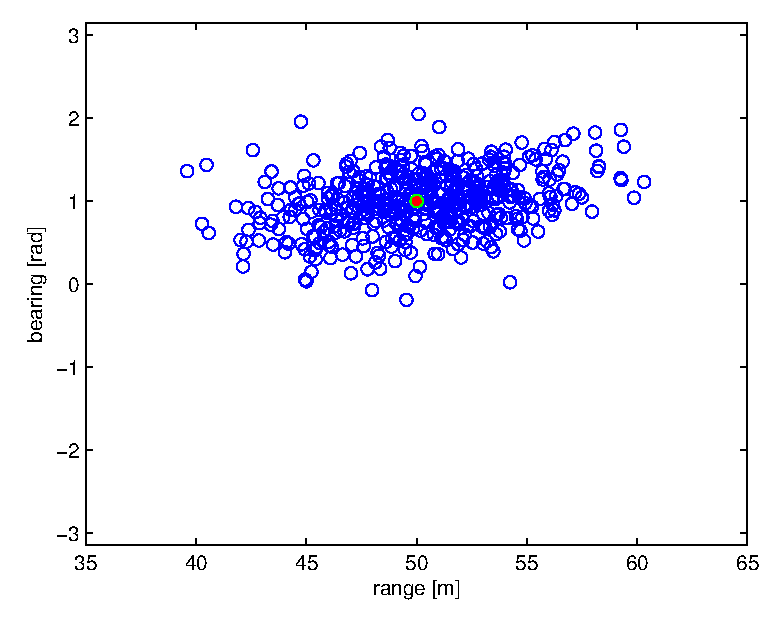
\includegraphics[width=0.40\textwidth]{kalman/fig/orig.eps}}
    \subfigure[Gaussian variable after nonlinear transform with mean and variance (ellipse) estimated using linearisation of the transform.]
    {\label{fig:lin-approx}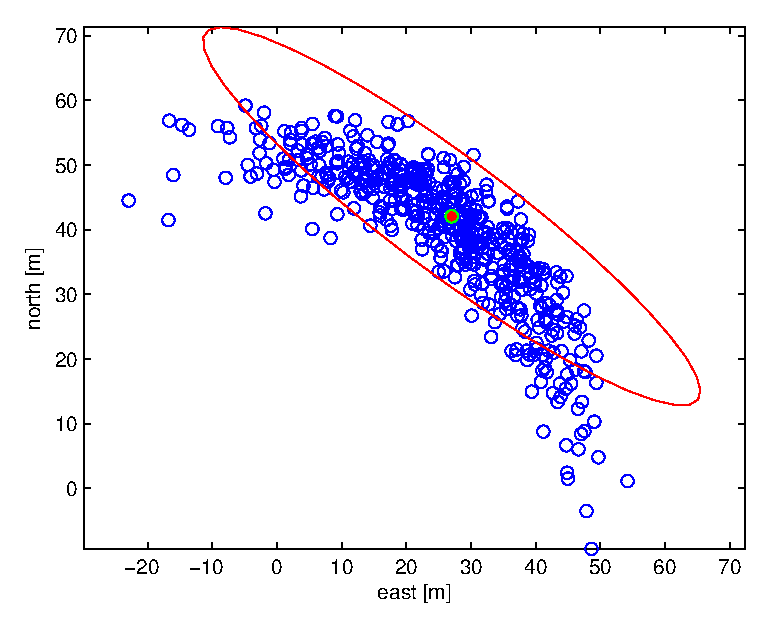
\includegraphics[width=0.40\textwidth]{kalman/fig/linear.eps}}      \\
    \subfigure[Original Gaussian random variable with samples selected by unscented transform algorithm.]
    {\label{fig:sigma-samples}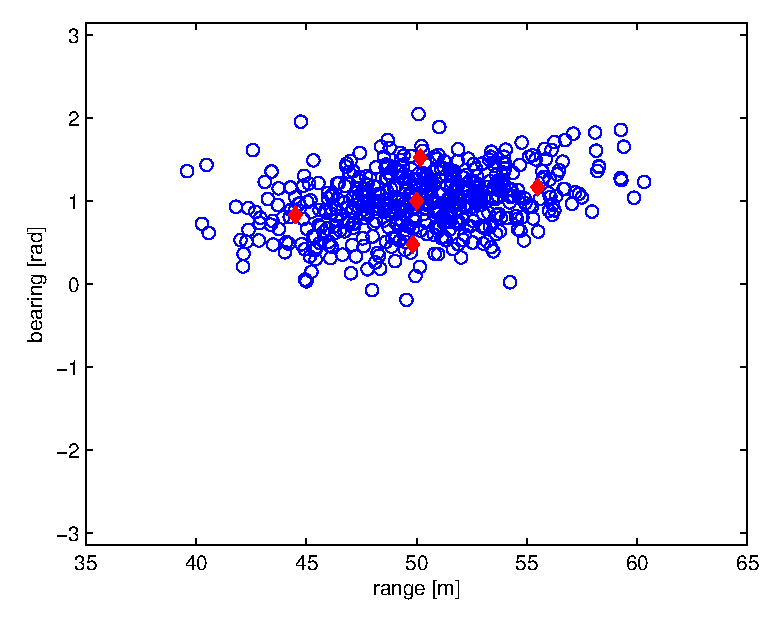
\includegraphics[width=0.40\textwidth]{kalman/fig/orig-samples.eps}}
    \subfigure[Gaussian variable after nonlinear transform with mean and variance (ellipse) estimated using unscented transform.]
    {\label{fig:unsc-transform}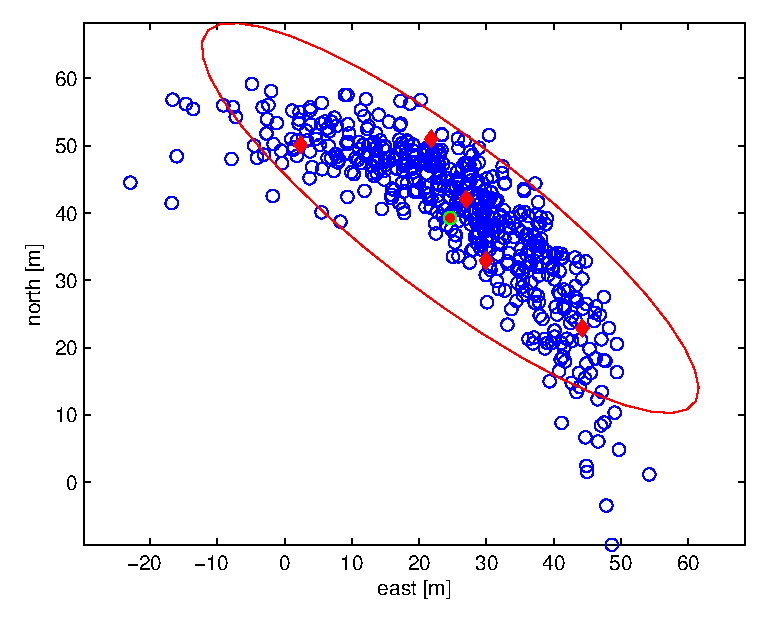
\includegraphics[width=0.40\textwidth]{kalman/fig/unscented.eps}}
  \end{center}
  \caption{Nonlinear transformation of a Gaussian random variable and estimation of its statistical parameters - mean and variance, using linearisation approximation and unscented transform.}
  \label{fig:gauss-transform}
\end{figure}

Calculation-wise, the whole procedure is fairly easier compared with linearisation algorithm since there is no need for calculating the Jacobian or Hessian, total number of computations stays the same and it is easier to improvise with the algorithm with constrains or parameters which define the way samples are selected. In addition, UT shown in example (Figure ~\ref{fig:gauss-transform} ) handles the whole distribution and its transformation by tracking only five samples. Higher dimensionality of GRV would result in more samples taken. However that number is still reasonably small compared with Monte Carlo methods. The only difficulty in implementation could be the non-trivial solution of the square root of the matrix as the necessary stage in unscented transform computation (Equation ~\ref{eq:ut-sampling} ).
\begin{algorithm}%[h!]
\caption{The Discrete Unscented Kalman Filter} \label{alg:ukf}
\begin{algorithmic}
\REQUIRE $\vect{\hat{x}}(0) = E\lbrace \vect{x}(0) \rbrace$
\COMMENT{initialize state}
\REQUIRE $\vect{P}(0) = \delta_{jk} \vect{P}_{0} $ 
\COMMENT {initialize covariance}
\REQUIRE $\vect{\hat{x}}^{aug}(0) = \left[ \begin{array}{c} \vect{\hat{x}}^{x}(0) \\ \vect{x}^{n}(0) \\ \vect{x}^{m}(0) \end{array} \right]
                                  = \left[ \begin{array}{c} \vect{\hat{x}}(0) \\ \vect{0} \\ \vect{0} \end{array} \right] $ 
\COMMENT{init. augmented state: state + process noise + meas. noise}
\STATE   $L = length(\vect{\hat{x}}^{aug}) \; k = const$
\COMMENT{augmented state length and $k$ parameter set}
\REQUIRE $\vect{P}^{aug}(0) = \left[ \begin{array}{ccc} \vect{P}_{0} & \vect{0}     & \vect{0} \\ 
															\vect{0} & \vect{P}_{n} & \vect{0} \\
															\vect{0} & \vect{0}     & \vect{P}_{m} \end{array} \right] $ 
\COMMENT{initialize augmented state covariance}
\LOOP
	\STATE $k \Leftarrow k+1$
	\STATE $\vect{A}^{aug}(k-1) = \left[\vect{\hat{x}}^{aug}(k-1) \vect{\hat{x}}^{aug}(k-1)\pm \sqrt{(L)\vect{P}^{aug}(k-1)}  \right] $
	\COMMENT {compute samples - unscented transform}
	\STATE   $ \vect{W}_{i}, \; i = 0,...,2L $
	\COMMENT {compute weights}
	\STATE   $\vect{A}^{x}(k \mid k-1) = f(vect{A}^{x}(k-1), vect{A}^{n}(k-1)) $
	\COMMENT {nonlinear process model}
	\STATE	 $ \vect{\hat{x}}(k \mid k-1) = \sum_{i=0}^{2L} \vect{W}_{i} \vect{A}^{x}_{i}(k \mid k-1) $
	\COMMENT {state prediction}
	\STATE   $ \vect{P}(k \mid k-1) = \sum_{i=0}^{2L} \vect{W}_{i} (\vect{A}^{x}_{i}(k \mid k-1) - \vect{\hat{x}}(k \mid k-1)) 
																   (\vect{A}^{x}_{i}(k \mid k-1) - \vect{\hat{x}}(k \mid k-1))^{T} $
	\COMMENT {state prediction uncertainty}
	\STATE   $\vect{Z}(k \mid k-1) = h(vect{A}^{x}(k-1), vect{A}^{m}(k-1)) $
	\COMMENT {nonlinear measurement model}
	\STATE   $\vect{\hat{Z}}(k) =  \sum_{i=0}^{2L} \vect{W}_{i} \vect{Z}_{i}(k \mid k-1)$
	\COMMENT {measurement prediction - unscented transform}
	\STATE   $\vect{P}_{zz} =  \sum_{i=0}^{2L} \vect{W}_{i} (\vect{Z}_{i}(k \mid k-1)-\vect{\hat{Z}}(k)) 
															(\vect{Z}_{i}(k \mid k-1)-\vect{\hat{Z}}(k))^{T}$
	\STATE   $\vect{P}_{xz} =  \sum_{i=0}^{2L} \vect{W}_{i} (\vect{A}_{i}(k \mid k-1)-\vect{\hat{x}}(k \mid k-1))
															(\vect{Z}_{i}(k \mid k-1)-\vect{\hat{Z}}(k))^{T}$
	\STATE   $\vect{K}      = \vect{P}_{xz} \vect{P}_{zz}^{-1}$
	\STATE	 $ \vect{\hat{x}}(k) = \vect{\hat{x}}(k \mid k-1) + \vect{K} (\vect{z}(k) - \vect{\hat{Z}}(k))  $
	\COMMENT {state correction}
	\STATE   $ \vect{P}(k) = \vect{P}(k \mid k-1) - \vect{K} \vect{P}_{zz} \vect{K}^{T} $
	\COMMENT {state correction uncertainty}	
	\RETURN $\vect{\hat{x}}(k), \vect{P}(k)$
\ENDLOOP
\end{algorithmic}
\end{algorithm}

\subsection{Monte Carlo-based filtering methods}
Monte Carlo methods, based on repeated random sampling as a part of the results computation are covered in several works, mostly dealing with Particle Filters (PF). Gordon et al. enclose \textit{bootstrap filter} \cite{gordon93}, also known as Particle Filter (PF) - a recursive algorithm based on representing state vector as set of random samples which are updated and propagated. Update stage of such algorithm uses Bayes rule, however the sampling strategy implies that the state space grid is not necessary the samples are localized in regions of high probability density \cite{gordon93}. Arulampalam et al. review Bayesian algorithms for nonlinear or non Gaussian problems. The emphasis of the review is on Particle Filters (PF), their features, variants and, finally, inevitable comparison with the standard EKF \cite{arulampalam02}. Doucet in his book on Monte Carlo methods \cite{doucet01} focuses on creating an broad summary of theory and various applications of bootstrap filters, optimal Monte Carlo filters and Particle Filters. Common feature of both ``Unscented'' and ``Monte Carlo Method'' estimation techniques is the sampling phenomenon. By using sampling, linearisation of plant and observation models is avoided, hence the cause of approximation error that existed in EKF-based methods is cancelled this way. PF can handle non Gaussian and and nonlinear processes, particularly exhibited in AUV models. Moreover, PF does not need to have the initial information about the state. Sampling techniques, particularly PF, have been recently and increasingly applied as tool for navigation of an underwater vehicle.

Karlsson et al. study a sea navigation method that relies on the underwater maps (depth map) and sonar measurements that support the navigation system \cite{karlsson02}. Particle Filter is used for state estimation. Since the problem of underwater navigation using depth map is nonlinear, sequential Monte Carlo methods are used, therefore state probability density is approximated with set of particles where each particle has a location and weight assigned to it. Both values reflect the value of the density of the region in the state space \cite{karlsson02}. Hence, instead of updating mean and covariance of the state, particle location and the weight of each particle are updated with each observation using sampling importance resampling (SIR) algorithm \cite{karlsson02}, \cite{gordon93}. Prior to navigation, terrain map (reference) was created using sonar depth measurements together with the Differential GPS measurements and the obtained grid was used for navigation. Moreover, the usage of Cram\'{e}r-Rao bound was investigated in tasks such as INS system design, sensor performance or even the amount of control of that is needed for the navigation. This work presents a successful application of particle filtering for underwater navigation.

Above-mentioned work of Di Massa \cite{diMassa97} presents navigation guided by the depth measured with bathymetric sonar. Map-matching with digital bathymetric map stored on-board has been accomplished using the Probabilistic Data Association Filter (PDAF) - a recursive algorithm similar to Kalman filter, designed for one target of interest and several measurements of the target state available each time step \cite{diMassa97}. Position within the bathymetric map was stored as the state vector that was filtered. Results proved that such navigation is possible and that having a more diverse sea floor leads to more accurate navigation.

Maurelli et al. \cite{maurelli08} propose a particle filter based underwater vehicle localization method for both structured and unstructured environment. Mechanically scanned profiling sonar is used as sensory device which provides information on distances from surrounding objects in environment. There is no information about initial position and orientation of the vehicle prior to localization. The work explores the possibility of dealing with dynamical situations when carrying out the localization results in movements of the vehicle that contribute in improving the particle filter algorithm output - active localisation. Improvements of the PF algorithm concern computational efficiency and effective way of treating state space in order to recover from wrong convergence when using PFs. Simulation and real experimental results are available.

\subsection{GPS aided localisation}
Caiti explored localization technique that uses floating acoustic buoys provided with GPS connection \cite{caiti05}. Idea is that buoys supply the vehicle with their GPS location by emitting the information at regular time intervals. This way, vehicle can calculate the time of flight of the acoustic signal and locate itself with respect to the buoys. In such constellation, additional equipment has to be installed and maintained. Furthermore, acoustic signals are not reliable, their range is limited and signals not always available. 

Erol \cite{erol07} proposes a method for localization of the network of underwater sensors using single AUV as aiding device. This is just one of the examples of utilization of knowledge on AUV location. The aim is to use it to maintain localization of group of other objects in the water such as acoustic sensors. It is a system where AUV initially and occasionally receives GPS signals while being on the surface. Once the GPS location is received, vehicle dives to a certain depth and follows the defined path in between the sensor network. Set of freely deployed acoustic sensors is receiving messages containing coordinates from the vehicle, since the vehicle maintains updating its position using dead reckoning combined with occasional GPS correction. Emphasis is on algorithms for distance estimation so that proper values for sensor coordinates can be passed on to sensor network localization algorithm.
\subsection{Localisation using \textit{a-priori} map}
Eustice experiments with re-navigation for AUVs \cite{eustice05towards}. The aim is to use a-priori given, ship derived bathymetric maps to reduce dead reckoning drift by comparing ship-derived depth map with the depth map created by vehicle. The difference between them is used as correction, a tool for removing long-term drift. 

Williams is presenting a new method that uses terrain features for aiding the tracking of underwater vehicles in unstructured environments \cite{williams06}. Benefit of such research lies in creating a vehicle capable of adopting to terrain changes therefore capable of being reliably deployed for longer time deep underwater, on a real task, with real environment. This work is revolutionary in solving the position update for a vehicle. Most common solution is the usage of acoustic transponders and triangulation algorithm as already exposed in Chapter \S~\ref{chap:capabilities}. Williams uses a priori elevation maps of the sea floor, recorded by ships. Depth information obtained from such mapping is assisting the localization process. Localization uses Monte Carlo methods, particularly PF, to manage map-based localization with position and velocity kept within state vector. Non-Gaussian estimates obtained using particles are bounded using depth and altitude observations by using range information to rule out less probable particles. Update is accomplished by resampling the particle distribution with respect to likeliness that the observation detected is received, given the sample of the state space \cite{williams06}. Apart form dealing with non-Gaussian estimates, advantages of such method include ability to track more than one possible target placement, which proves to be useful feature when handling map-based information.  
%%%%%%%%% A-PRIORI LANDMARKS CONSTRUCTED USING SENSOR DATA %%%%%%%%%%%%
Newman and Durrant-Whyte propose a navigation filter which uses inertial measurement unit (IMU) and sonar to carry out the terrain-aided navigation \cite{newman98}. IMU is used to measure the kinematic parameters such as accelerations and rotations with respect to body frame, while sonar measures absolute distances and orientations with respect to the world frame. In such configuration, sonar system does the correction of the noise-corrupted, drift-prone position indicated by IMU. Standard Kalman filter is used to integrate different sensor measurements with a-priori dynamics model of the vehicle. Sonar observations are processed with target extraction algorithm isolating terrain beacons. Map is simultaneously created during the vehicle mission. It map serves as the representation of the world and contains distinctive features from environment. Map is intended to be a sparse world representation, containing least possible but still enough information (features) to make a reference to and it is derived from estimation of the floor gradient using sonar measurements. Pose observation is defined relative to features from the map that correspond to features from the real world.

Similarly, Williams et al. present the results of operational algorithm that processes sonar scans in order to extract robust features of the environment further used to build an environment map consisting of those features \cite{williams00}. The vehicle location is estimated within the built environment map. The work is an example of practical application of SLAM (Section \S~\ref{sec:slam}).

Another contribution of Eustice \cite{eustice05exactly}, based on vehicle localization with simultaneous terrain-features map creation (SLAM), reports usage of delayed state model. Robot movement is observed with respect to its previous position. Benefit of the delayed state framework lies in having precisely sparse information matrix. Main idea of the work is that, unlike previous algorithms, sparseness of the SLAM information matrix used in localization is guaranteed, not approximated.
%%%%%%%%% TERRAIN-AIDED WHEN TASK IS ACHIEVED %%%%%%%%%%%%
%%%%%%%%% OTHER THAN TIME-OF-FLY %%%%%%%%%%
%%%%%%%%% OPTICAL SENSING %%%%%%%%%%%%%
\subsection{Optical sensing}
Tena Ruiz investigates terrain aided localization of an AUV from the perspective of Simultaneous Localization and Mapping (SLAM) \cite{ruiz01}. Sonar device is used to sense the environment and its readings are used to find targets located not far from the vehicle. SLAM algorithm uses detected targets together with a vehicle model to simultaneously construct the environment map and localize the vehicle using filtering. Multiple Hypothesis Tracking Filter is adjusted to the SLAM framework. Necessary step of matching the sonar images with environment targets was accomplished by extracting the features and associating them with the sonar recordings by calculating a score that expresses the probability of a certain target causing a certain sonar output. 

Williams presents the results of sonar usage together with the vision based system in SLAM algorithm for terrain-aided navigation \cite{williams04}. Seabed covered with visually distinctive textured reefs was used in estimating vehicle motion and creating a map of the reef structure.  

Eustice proposes several works on vision based localisation for AUVs in an unstructured undersea environment. Framework presented in \cite{eustice04} blends together sensor data and camera measurements in order to determine the relative pose. The final aim is to concurrently determine the vehicle position and the past trajectory \cite{eustice04}. Augmented state Kalman filter is used to filter out the pose of the vehicle. History of poses defines vehicle trajectory. Registered images obtained with camera provide spatial constraints for the position hence providing the necessary feedback for pose estimation. Moreover, the registration of the image pairs is more robust compared with the situation when only camera is used for sensing. The other vision based SLAM approach \cite{eustice05} addresses the problem of localization within large areas. Precise localization is a prerequisite for high resolution underwater imaging of large objects placed on the sea-bed \cite{eustice05}. Precise navigation would enable decent coverage of the spacious site of interest which is mission task. Proposed solution uses a vision-based SLAM approach together with vehicle's inertial sensors' measurements. The originality of the paper is that it suggests a genuine solution for evaluating covariance bounds within the EKF used for filtering SLAM information. 

Carreras \cite{carreras03} experiments with the usage of visual information for underwater robot localisation within the pool with clear visibility. This method is not intended for ocean environment, however, it is useful from the computer-vision side and potentially a tool to aid video mosaicking algorithms. Camera is mounted on the vehicle and used to simultaneously record the bottom of the tank covered with the coded pattern. This way, structured environment is used for, map-based 3D localisation of the vehicle. Number of computer-vision related matters are examined, such as: necessary camera calibration, filtering methods, landmark detection. Localisation performance is reported to be high, with high computation rate and, importantly, prone to drift. Hence, reliable position information is good enough to derive the velocity estimates from it. In addition, work contains the analysis of the source of localisation errors and real time application examples.  
%%%%%%%%%%%%%%%% SLAM BASED %%%%%%%%%%%%%%%%%%%%%%%%%%%
\subsection{Simultaneous location and mapping}
In order to deal with SLAM issues, several methodologies are covered in literature. View-based approach generally relies on registering different types of imagery: optical imagery or depth imagery in order to establish spatial constraints that are vision-based, therefore, not prone to drift error (\cite{garcia01, eustice05towards, roman05}). This approach does not include precise representation of features. SLAM frameworks that, however, use features (feature-based) instead of view are reported in (\cite{williams04, ruiz01}).
%%%%%%% COMMUNICATION COOPERATIVE NAV PAPERS %%%%%%%%%%
\subsection{Cooperative navigation}
The dissertation of Bahr (\cite{bahr08}) focuses on cooperative navigation, and furthermore, general background on localisation is surveyed. Bahr proposes a probabilistic-based algorithm, particularly tailored to the underwater environment. Cooperation in navigation is already available in air or the surface of the Earth. The work focuses on cooperative localization where different vehicles, arranged in group, communicate between each other. To accomplish cooperative localization, algorithm estimates inter vehicle range, resulting in position and the uncertainty of the position, then exchanges that information with other vehicles. Main idea is to exchange  localisation-related information. The whole process consists of data acquisition and data processing stage. Forward propagation of position information causes more than one solution available. Further data processing gives an estimate of the location by processing all the possibilities. Stated advantages of such approach are that, apart from having more than one vehicle, no additional infrastructure is necessary \cite{bahr08}. Everything comes down to the usual sensor and communication package already available on vehicles\cite{bahr08}. 
%They use it together with the localisation data received from the other vehicles to make corrections of the position and position covariance.

Fallon et al. \cite{fallon10} describe the implementation of the cooperative localisation algorithm that works within group of AUV vehicles, aided with the position information from the autonomous surface vehicle to bound the estimation errors. Instead of the usage of expensive navigation sensors for communicating under the water surface, an approach where cooperation with one surface vehicle was suggested. Surface vehicle is intended to contribute with accurate position information. One of the contributions of the work is a trial of EKF localisation run on AUV and supported by the surface vehicle moving along with the AUV. Work investigates the usage of different estimators - Particle Filters, non-linear Least-Squares Optimization (NLS) and EKF in cooperation localisation within a mission consisting of two AUVs and one surface vehicle. It ends up comparing performance of each algorithm with the final outcome giving more credits to PF and NLS. 
%\chapter{State of the art} \label{chap:state-of-the-art}

This chapter gives an overview of the methods and existing algorithms for underwater vehicle localization. Localization is influenced with the development sensor devices. Sensors can be regarded as the tool for managing the localization. Faster they are, more accurate they are, localization has more chances to be better. Chapter \S~\ref{chap:sensors} gives more insight into performance of each sensor device used for underwater vehicle navigation. Following paragraphs are revising the ways to process such sensor information. We could describe localization as absolute or relative, depending on which reference system we use when obtaining measurements - environment or the vehicle itself. 

In existing survey on underwater vehicle navigation, Kingsey et al. \cite{kinsey06} already give a summary presenting some methods used. As introduced in \cite{kinsey06}, current vehicle position is named navigation state - a vector where the vehicle is and how it is oriented in space. Localization simply means finding a way to estimate navigation state vector. Naturally, sonsors provide the data for estimation.

The most simple approach would be to take the raw sensor measurements and use them directly or within a simple mathematical model that describes the vehicle dynamics. However, many techniques utilize sensor data as supplementary information with the information from the kinematic model. Rough classification would categorize localization methods on stochastic state estimators (Section ~\ref{sec:stochastic-methods}), simultaneous localization and mapping approach (SLAM, Section ~\ref{sec:slam} and localization based on deterministic observers \cite{kinsey06}.

\section{Stochastic state estimators} \label{sec:stochastic-methods}
The name of such methods suggests that states are treated as ultimately having feature of randomness built-in. As it is the case with random variables, we can say that certain state has an expected value, and that such randomness can be expressed with the distribution formula. This approach is hitorically. Most notable stachastic state estimator is Kalman filter. Kalman filter is an unbiased, optimal estimator which treats random variable as it has gaussian distribution. In case of an underwater vehicle localization is accomplished using Kalman Filter (KF) or an Extended Kalman Filter (EKF). Several works report on usage of Kalman filters for state estimation. 

Kalman filter output could be corrupted in situations when observations (sensor measurements) are subject to interruption or periodic stopping. Due to the fact that not all the sensors can be always available, it is usually necessary to be capable of adding or removing sensor observations from the system without changing the navigation algorithm. 

Blain et al. \cite{blain03} study application of Kalman filter in navigation of an underwater vehicle used for water dam inspection merging position and velocity information. This example uses acoustic positioning sensor to measure the position directly and the integration the DVL sensor velocities \cite{blain03}  asynchronous data delivery and delays in measurements


Drolet et al. \cite{drolet00} introduce a flexible localization strategy based on sensor fusion and usage of several Kalman filters arranged together in a bank. Each filter is reduced to express simple cinematic equation and processes one state - works in one dimension. Idea is to integrate together sensor measurements that arrive at different time moments from different sensors. Method takes asynchronous information from sensors, manages a filter switching process so that the most recent data is used to update those filters that can be updated with such measurement \cite{drolet00}. Such sensor fusion strategy is adaptable in terms of number of sensors so that the best is taken out from the available input data, more robust to data loss. Moreover, asynchronous inputs are allowed. 

\cite{diMassa97}
\cite{gade99}
\cite{eustice05}
\cite{roman05}
\cite{yun00}
\section{SLAM} \label{sec:slam}

\section{Deterministic state estimators}
 





\chapter{Methodology} \label{chap:methodology}
Position, orientation and velocities of a vehicle underwater are stored within the state vector. Proposed solution for localization uses state-space approach and Extended Kalman Filter to estimate the value of the state vector using data from odometry sensors and acoustic positioning system (LBL), if available. Data are merged together using the EKF. Reasons for choosing this method are influenced by the application itself. Localisation is intended to work in unstructured environments, with no clear visibility, relying on kinetic and absolute position measurements. Therefore, approaches that use vision, or capture the terrain structure in order to aid the navigation were not an adequate solution. Relying on the remaining sensor configuration allows the usage of Kalman filter to iteratively and recursively estimate the state vector by combining together different types of dynamics-related data. State-space approach is convenient for manipulation with multivariate data and nonlinear or non Gaussian processes \cite{ristic04}. 

Mathematical model of the system is the integral part of the Kalman filter. It is used to define the state transition law by applying well known kinematic equations.  Kinematic equations describe the object motion. \textit{Constant velocity} kinematic model is used as system model to predict the movements of the submerged body. States are predicted at each time-step using the model and previous state (equation ~\ref{eq:state-tran}). It is important to note that localization comes down to solving non-linear filtering problem. System model equations are nonlinear function of the state elements. Sensor measurements are used when available and incorporated into observation (measurement) in order to update and correct the predicted filter state. Range of available sensors give information on vehicle's current location state. Overview of the sensors and the values that they measure is given in Chapter \S~\ref{chap:sensors}.
\section{Process model} \label{sec:system-model}
5DOF system model is used to describe the state transition in time. In proposed discrete-time stochastic model, five degrees of freedom include position values and two angle states: yaw and pitch - making altogether five possible values to change in modelling vehicle position (figure ~\ref{fig:auv-positioning}). Since the application uses state-space approach, focus will be on defining a state vector that would incorporate all the relevant values for the dynamic system that does the localisation - kinematic and position variables. In spirit of that, system state vector combines together metric and angular values. At discrete time moment $k$, it values:
$$ \vect{X}(k) = 
\left[ 
\begin{array}{ccccccccccc}
x & y & z & a & u & v & w & \psi & \varphi & \dot{\psi} & \dot{\varphi}
\end{array}
\right] ^{T} $$  
where $x$ takes the value of \textit{north} (expressed in meters), $y$ is \textit{east} and $z$ is \textit{depth}. Inspiration for marking the variables with these letters was taken from \cite{ribas10}. Further on, $a$ marks the \textit{altitude} with $u$, $v$ and $w$ standing for linear velocities: \textit{surge velocity}, \textit{sway velocity} and \textit{heave velocity}, respectfully. The rest of the state vector covers angular values (expressed in radians or degrees). $\psi$ and $\varphi$ are used as yaw and pitch, hence describing the vehicle orientation. $\dot{\psi}$ and $\dot{\varphi}$ are angular velocities: yaw rate and pitch rate, respectfully. The state vector incorporates all the relevant information necessary to describe the system under investigation. Angle and velocity for pitch degree of freedom is included in 5DOF system model since it can make a difference in estimating vehicle location in certain movement scenarios (figure ~\ref{fig:motion-scenario}). System model is describing how the state $\vect{X}$ evolves in time. It is defined as constant speed model that uses previous state and noise to make a prediction on the next state vector value $\vect{X}(k)$  using non-linear function $f()$ and process noise vector $\vect{n}$ (equation ~\ref{eq:state-tran}) where $\vect{N} = \left[ \begin{array}{ccccc} \dot{u} & \dot{v} & \dot{w} & \ddot{\psi} & \ddot{\varphi} \end{array} \right]^{T}$. Process noise models inaccuracies or unpredictable disturbances in motion model \cite{ristic04}. 
\begin{equation}
\vect{X}(k) = f(\vect{X}(k-1), \vect{N}(k-1))
\label{eq:state-tran}
\end{equation}

\begin{equation}
\begin{bmatrix} x \\ y \\ z \\ a \\ u \\ v \\ w \\ \psi \\ \varphi \\ \dot{\psi} \\ \dot{\varphi} \end{bmatrix}_{(k)} =
\begin{bmatrix} x + (uT+\dot{u}\frac{T^{2}}{2})\cos(\psi)\cos(\varphi) - (vT+\dot{v}\frac{T^{2}}{2})\sin(\psi)\cos(\varphi) \\ 
                y + (uT+\dot{u}\frac{T^{2}}{2})\sin(\psi)\cos(\varphi) + (vT+\dot{v}\frac{T^{2}}{2})\cos(\psi)\cos(\varphi) \\ 
                z + (wT+\dot{w}\frac{T^{2}}{2})\cos(\varphi) \\ 
                a - (wT+\dot{w}\frac{T^{2}}{2})\cos(\varphi) \\ 
                u + \dot{u}T \\ 
                v + \dot{v}T \\ 
                w + \dot{w}T \\ 
                \psi    + \dot{\psi}T    + \ddot{\psi}   \frac{T^{2}}{2} \\ 
                \varphi + \dot{\varphi}T + \ddot{\varphi}\frac{T^{2}}{2} \\ 
                \dot{\psi}    + \ddot{\psi}T \\ 
                \dot{\varphi} + \ddot{\varphi}T
\end{bmatrix}_{(k-1)} 
\label{eq:state-tran-matrix}
\end{equation}
To summarize, implementing vehicle localization using EKF demands establishment of two models: first one describing the state evolution (system model) and second model that associates noisy measurement with the state (measurement model). 
\begin{figure}%[htb]
  \centering
    \subfigure[AUV positioning - global frame of reference.] {\label{fig:auv-positioning}
	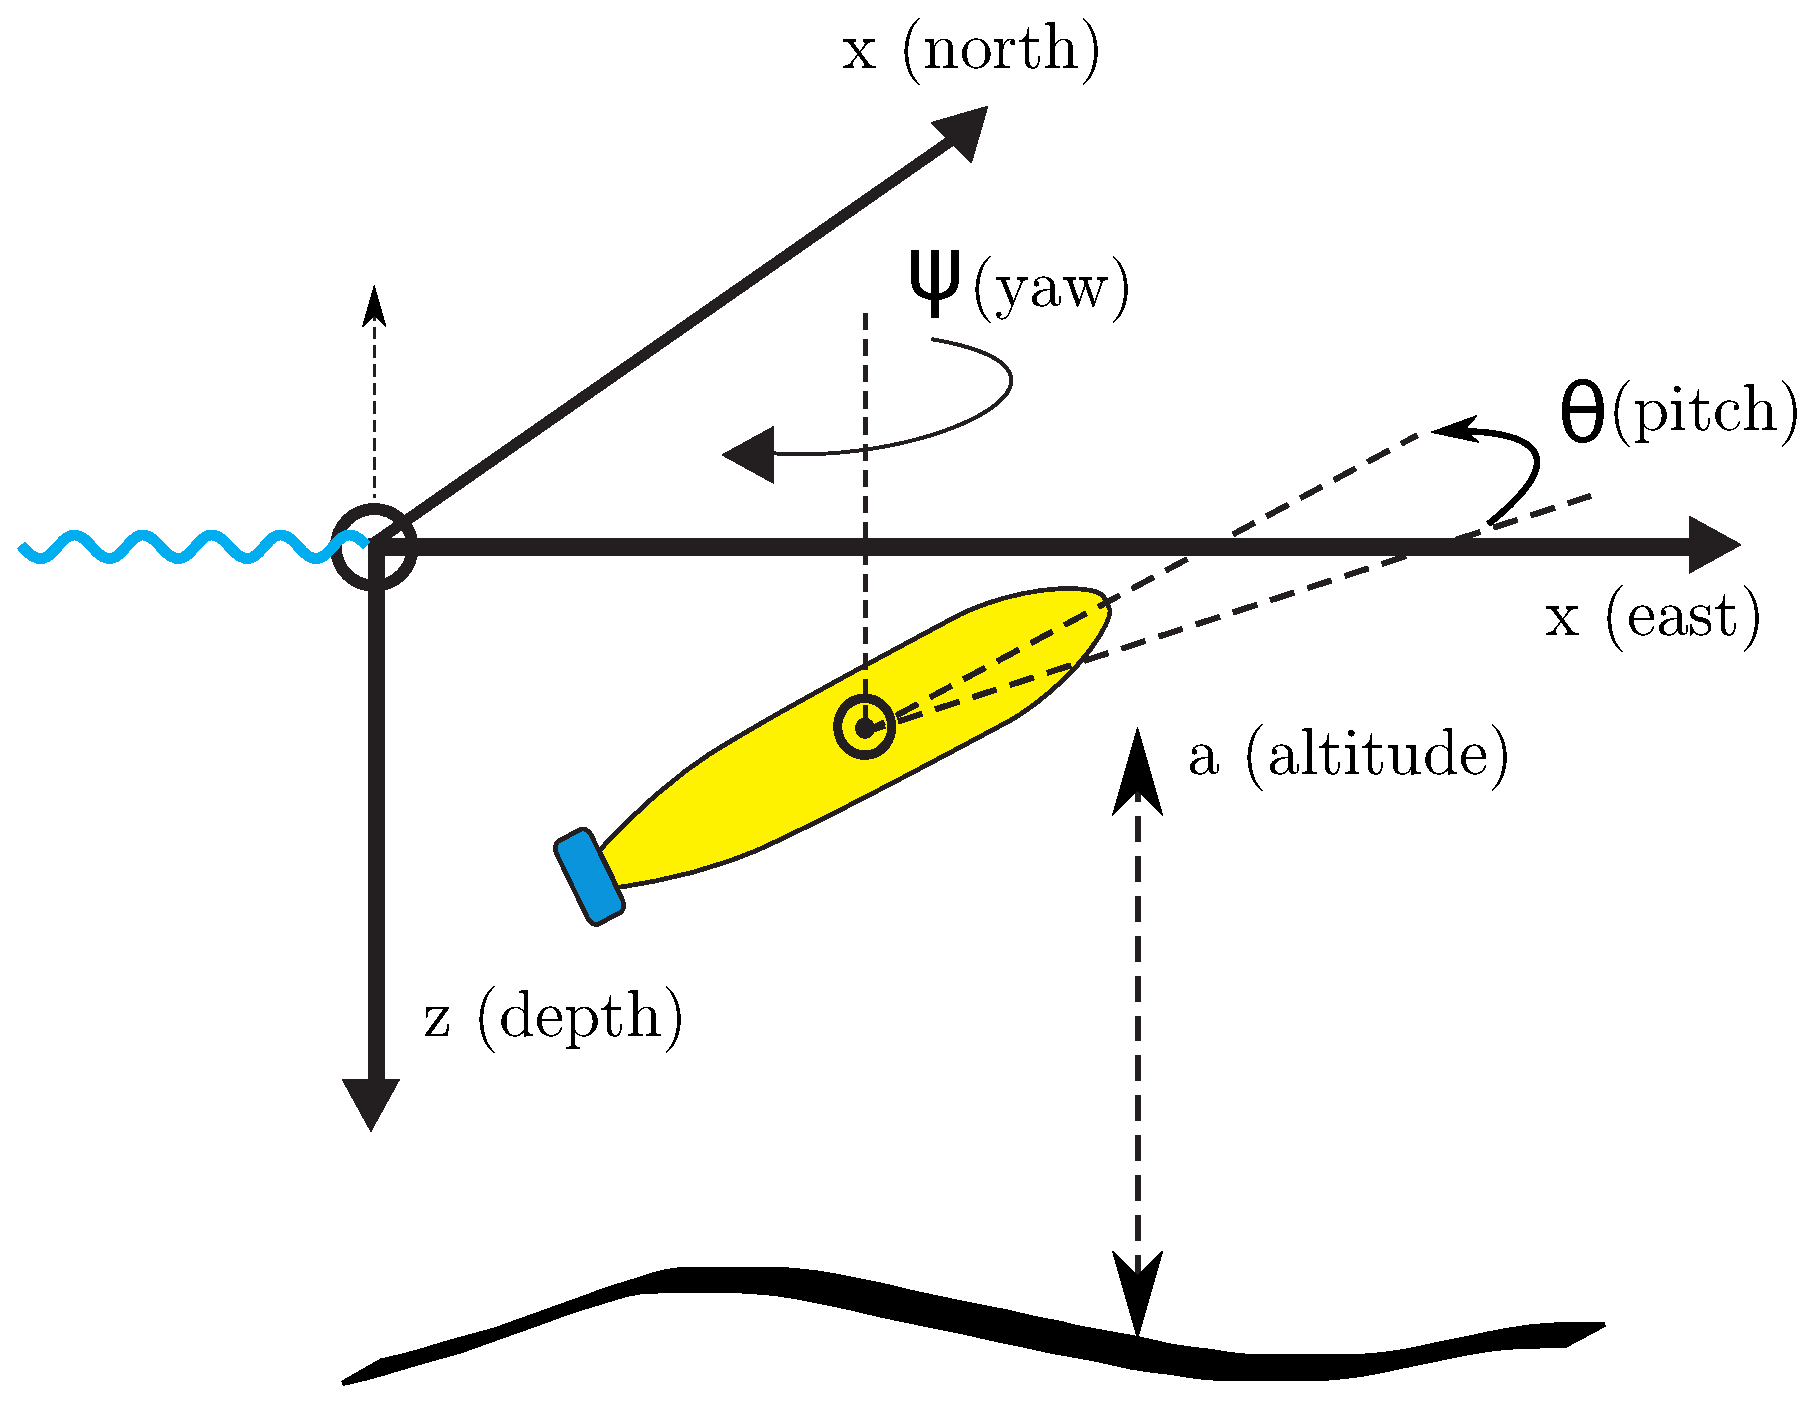
\includegraphics[width=0.40\linewidth]{methodology/fig/auv-model.eps}}
    \subfigure[AUV body frame - local coordinate system with movement directions.] {\label{fig:auv-axes}
    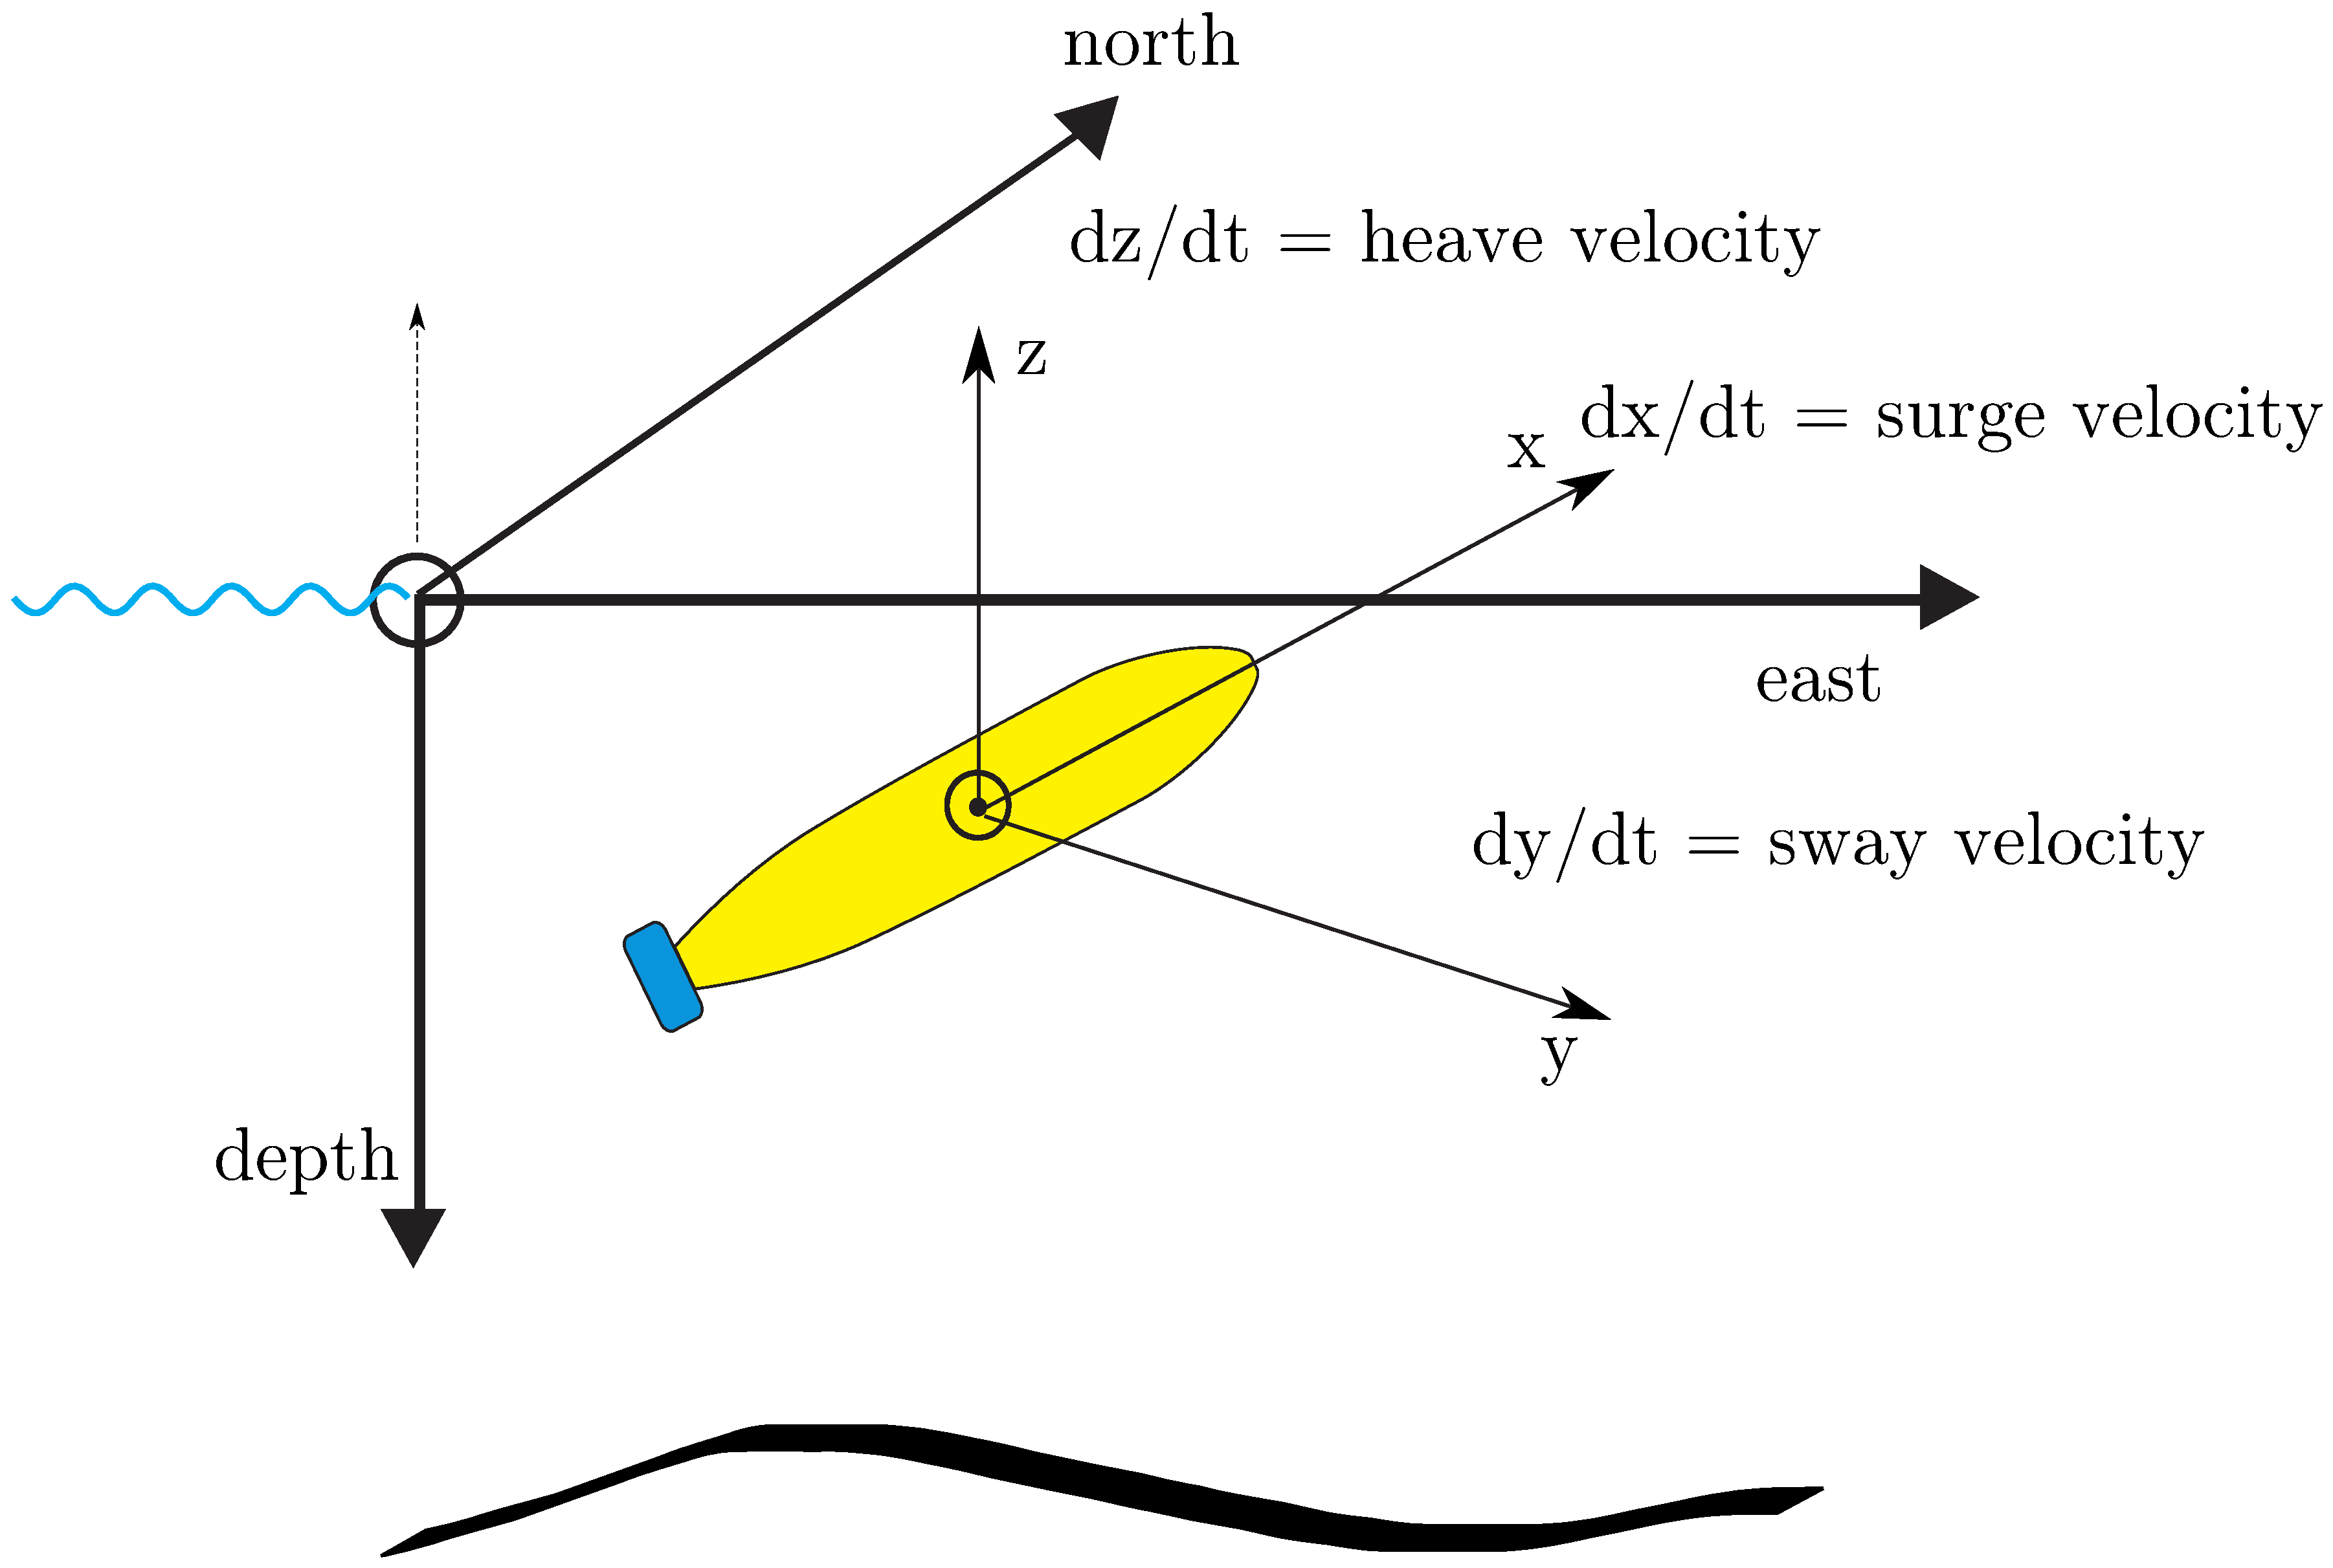
\includegraphics[width=0.40\linewidth]{methodology/fig/auv-axes.eps}} \\
    \subfigure[AUV pitch-influenced motion scenario.] {\label{fig:motion-scenario}
    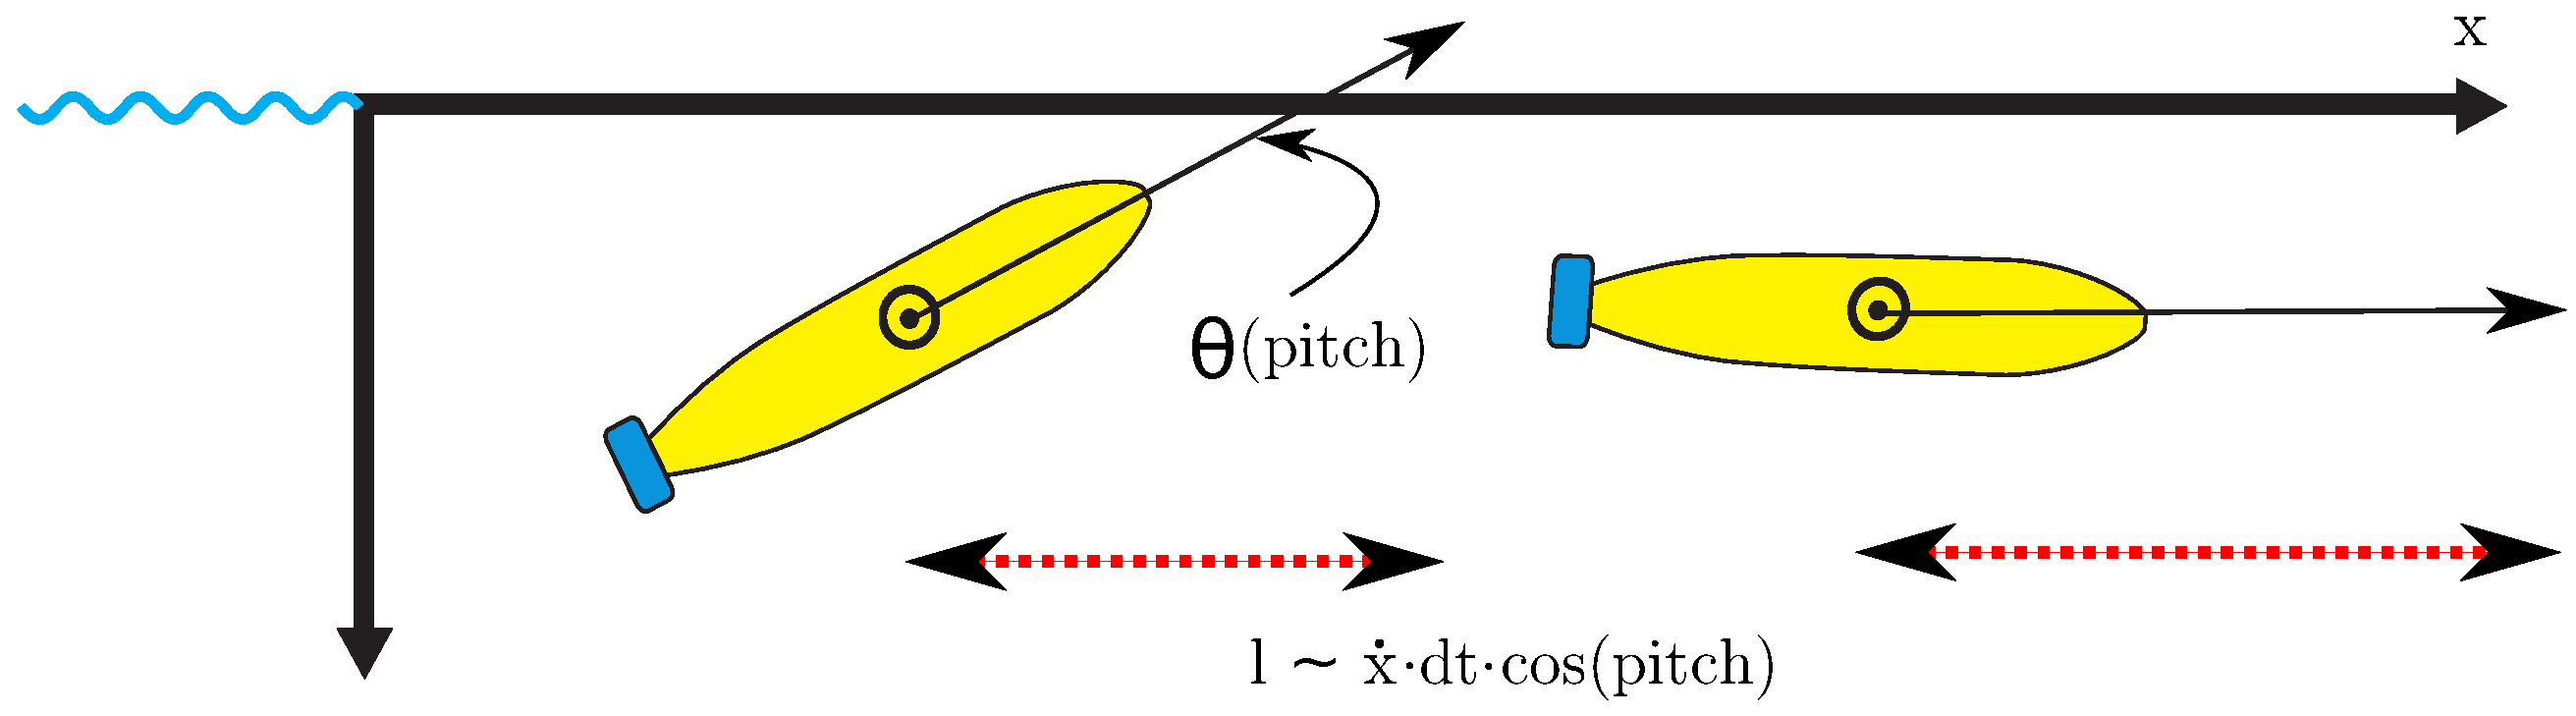
\includegraphics[width=0.5\linewidth]{methodology/fig/scenario.eps}}    
\caption{AUV state vector values and five degrees of freedom.}
\label{fig:auv-states}
\end{figure}

EKF (\S~\ref{sec:ekf}) was used in order to estimate the vehicle state vector. It was chosen as logic choice being an algorithm that integrates together different sensor measurements, makes a sub-optimal, recursive state estimation and above all, is derived for non-linear systems. As the theory of non-linear filtering suggests, state-space approach is used for modelling discrete-time dynamic system in this application. The main feature of EKF is that it linearises the system model and measurement model nonlinear functions. System model is further developed according to formulas ~\ref{eq:der-proc-state}, ~\ref{eq:der-proc-noise}, ~\ref{eq:der-mes-state} and ~\ref{eq:der-mes-noise} from Chapter on Nonlinear filtering \S~\ref{chap:methodology}, resulting in matrices:
\begin{align*}
\vect{F}(k) & = &  \frac{\partial f}{\partial X} (\vect{\hat{X}}(k \mid k-1), 0) & = & 
\end{align*}
\begin{footnotesize}
$$ \left[ 
\begin{array}{ccccccccccc}
1 & 0 & 0 & 0 & T c(\psi) c(\varphi) & -T s(\psi) c(\varphi) & 0 & -Tc(\varphi)(us(\psi)+vc(\psi)) & -Ts(\varphi)(uc(\psi)-vs(\psi)) & 0 & 0 \\
0 & 1 & 0 & 0 & T s(\psi) c(\varphi) & T c(\psi) c(\varphi) & 0 & Tc(\varphi)(uc(\psi)-vs(\psi)) & -Ts(\varphi)(us(\psi)-vc(\psi))  & 0 & 0 \\
0 & 0 & 1 & 0 & 0 & 0 &  Tc(\varphi) & 0 & -vTs(\varphi) & 0 & 0 \\
0 & 0 & 0 & 1 & 0 & 0 & -Tc(\varphi) & 0 &  vTs(\varphi) & 0 & 0 \\
0 & 0 & 0 & 0 & 1 & 0 & 0 & 0 & 0 & 0 & 0 \\
0 & 0 & 0 & 0 & 0 & 1 & 0 & 0 & 0 & 0 & 0 \\
0 & 0 & 0 & 0 & 0 & 0 & 1 & 0 & 0 & 0 & 0 \\
0 & 0 & 0 & 0 & 0 & 0 & 0 & 1 & 0 & T & 0 \\
0 & 0 & 0 & 0 & 0 & 0 & 0 & 0 & 1 & 0 & T \\
0 & 0 & 0 & 0 & 0 & 0 & 0 & 0 & 0 & 1 & 0 \\
0 & 0 & 0 & 0 & 0 & 0 & 0 & 0 & 0 & 0 & 1 \\
\end{array}
\right] $$ 
\end{footnotesize}
where $c(\psi)$ and $c(\varphi)$ stand for $\cos(\psi)$ and $\cos(\varphi)$ respectfully. Similarly, $s(\psi)$ and $s(\varphi)$ mark the angle sinuses.  
\begin{align*}
\vect{W}(k) & = & \frac{\partial f}{\partial N} (\vect{\hat{X}}(k \mid k-1), 0) & = &
\end{align*}
$$ 
\begin{bmatrix}
\frac{T^{2}}{2}\cos(\psi)\cos(\varphi) & -\frac{T^{2}}{2}\sin(\psi)\cos(\varphi) & 0 & 0 & 0 \\
\frac{T^{2}}{2}\sin(\psi)\cos(\varphi) &  \frac{T^{2}}{2}\cos(\psi)\cos(\varphi) & 0 & 0 & 0 \\
0 & 0 & \frac{T^{2}}{2}\cos(\varphi) & 0 & 0 \\
0 & 0 & -\frac{T^{2}}{2}\cos(\varphi) & 0 & 0 \\
T & 0 & 0 & 0 & 0 \\
0 & T & 0 & 0 & 0 \\
0 & 0 & T & 0 & 0 \\
0 & 0 & 0 & \frac{T^{2}}{2} & 0 \\
0 & 0 & 0 & 0 & \frac{T^{2}}{2} \\
0 & 0 & 0 & T & 0 \\
0 & 0 & 0 & 0 & T \\
\end{bmatrix}
$$
Knowing plant model and deriving $\vect{F}(k)$, $\vect{W}(k)$ enables EKF algorithm to complete the prediction stage using known formulas. Next step is correction of the prediction using data obtained from measurement.
\section{Measurement model} \label{sec:measurement-model}
Measurement model introduces measurement equation which establishes connection between the measurements and the target state (equation ~\ref{eq:mes-model}) where $Z(k)$ represents the measurement at time $k$, $X(k)$ represents state vector and $M(k)$ represents noise. Purpose of the measurement is to be able to update, correct the state $X(k)$ using measurements $Z(k)$. $h()$ is generally a non-linear function. EKF idea is to linearise measurement model.
\begin{align*}
\vect{H}(k) = \frac{\partial h}{\partial X} (\vect{\hat{X}}(k \mid k-1), 0) \\
\vect{R}(k) = \frac{\partial h}{\partial M} (\vect{\hat{X}}(k \mid k-1), 0)
\end{align*}
However, for this particular application and available sensor configuration, state vector elements are measured directly, hence $h()$ can be expressed with matrix containing ones at particular positions since the measurement relation becomes equality. There is no need for partial derivation. Measurement noise is submitted in form of additive Gaussian zero-mean noise assigned to each measured value. Measurement (observation) noise is characterised with zero mean $(E \lbrace \vect{M}(k) \rbrace = 0)$ and standard deviation $(E \lbrace \vect{M}(k) \vect{M}^{T}(k) \rbrace)$ given as filter parameter for each of the measurement. It expresses how uncertain or varying, measurement of each of the state values is. The measurement in vehicle configuration used for the thesis enables direct measurement of each of the states and each measurement of one of the state elements is described with its uncertainty - variance of the Gaussian noise. Variances are given as filter parameters saying how much we trust in the measurement.  
\begin{equation}
\vect{Z}(k) = h(\vect{X}(k), M(k)) = \vect{H} \vect{X}(k \mid k-1)  + \vect{M}(k)
\label{eq:mes-model}
\end{equation}
One of the features of EKF localization for an AUV is that measurements are not available all the time. Reason is the nature of the process of estimating localization itself. Simply - messages from sensors arrive at different moments and it happens that some of the sensors could not be available due to different causes. The idea is to take all the available information at the moment of filtering and integrate it together in measurement model, as filter observation. Alternatively, each message can be filtered upon its arrival. As a result, filter would keep carrying out the prediction and correction blending together various measurements in a estimate of higher quality, with the ability to compensate the missing sensor measurements. 

A short overview of the sensor measurements and the pattern of formation of the measurement model is presented in following section. Idea for the solution has been introduced in \cite{ribas10}. Some other implementations of EKF for underwater navigation have reported the usage of similar strategy for merging the measurements together \cite{drolet00, blain03}. Sensors have been introduced with more details in chapter ~\ref{chap:sensors}. Linear observation model varies depending on the measured values and sensors used for the measurement. 
\begin{itemize}
\item \T{Pressure sensor}
periodically ``feeds'' the filter with depth and heave velocity information. Heave velocity information is derived from depth measurement by derivation of its value per elapsed time. Measurement model is linear, described with the transformation matrix $\vect{H}_{depth}$. Uncertainty of the measurement is expressed with measurement noise matrix $\vect{R}$ (\S~\ref{sec:kf}) - covariance of the measurement vector.  
\begin{equation}
\label{eq:press-mes}
\vect{H}_{depth}(k) = 
\left[ \begin{array}{ccccccccccc}
0 & 0 & 1 & 0 & 0 & 0 & 0 & 0 & 0 & 0 & 0 \\
0 & 0 & 0 & 0 & 0 & 0 & 1 & 0 & 0 & 0 & 0 \end{array} \right],
\vect{R}_{depth}(k) =  
\left[ \begin{array}{cc}
\sigma_{z}^{2} & 0 \\
0 & \sigma_{w}^{2} \end{array} \right]
\end{equation}
\item \T{Compass}
supplies angular measurements such as pitch, yaw, pitch rate (figure ~\ref{fig:auv-positioning}). Similarly as with pressure sensor measurement model, rate of change of pitch is obtained with derivation of pitch measurement. Measurement model is linear, described with the transformation matrix $\vect{H}_{compass}$. $\vect{R}_{compass}$ is measurement noise matrix (\S~\ref{sec:kf}) containing variances depicting Gaussian noise of particular measurements.
\begin{equation}
\label{eq:com-mes}
\vect{H}_{compass}(k) = 
\left[ \begin{array}{ccccccccccc}
0 & 0 & 0 & 0 & 0 & 0 & 0 & 0 & 1 & 0 & 0 \\
0 & 0 & 0 & 0 & 0 & 0 & 0 & 0 & 0 & 0 & 1 \\
0 & 0 & 0 & 0 & 0 & 0 & 0 & 1 & 0 & 0 & 0 \end{array} \right], 
\vect{R}_{compass}(k) =
\left[ \begin{array}{ccc}
\sigma_{\varphi}^{2} & 0 & 0 \\
0 & \sigma_{\dot{\varphi}}^{2} & 0 \\
0 &     0          & \sigma_{\psi}^{2} \end{array} \right]
\end{equation}
\item \T{Fiber-optic-gyroscope sensor (FOG)}
measures yaw rate $(\dot{\psi})$. FOG, unlike compass, gives an absolute measurement of the rate. In case of compass yaw rate is determined by doing derivation in time using previous yaw measurement. FOG turns out to be quite precise and fast sensor. Yaw rate can be used to determine the yaw (heading) itself by integrating the yaw rates over time. That would imply relative measurement of yaw - with respect to previous value. Relative measurements cannot correct the starting error, in case it existed.  Disadvantage of FOG usage for yaw measurement is that the initial heading value still needs to be given by compass, as an absolute measurement. This can result in constant bias of measured heading in case the initial heading was measured with an error. Error would propagate through relative measurements in form of the bias. Given that compass is prone to errors, this scenario is possible. Measurement model matrices are:
\begin{equation}
\label{eq:fog-mes}
\vect{H}_{fog}(k) = 
\left[ \begin{array}{ccccccccccc}
0 & 0 & 0 & 0 & 0 & 0 & 0 & 0 & 0 & 1 & 0  \end{array} \right], 
\vect{R}_{fog}(k) =
\left[ \begin{array}{c}
\sigma_{\dot{\psi}}^{2} \end{array} \right]
\end{equation}  
\item \T{Doppler Velocity Log (DVL)}
measures linear speeds - surge and sway velocities with respect to vehicle axes (Figure ~\ref{fig:auv-axes}) and the altitude. $\vect{H}_{dvl}$ and $\vect{R}_{dvl}$ are measurement and measurement noise matrices containing variances depicting Gaussian noise of particular measurements. If DVL gives no valid velocity output due to insufficient signal (DVL lock lost), EKF is using the available data available from other sensors to make an update or it is just maintaining the increasingly uncertain prediction part until the fresh observation arrives.    
\begin{equation}
\label{eq:dvl-mes}
\vect{H}_{dvl}(k) = 
\left[ \begin{array}{ccccccccccc}
0 & 0 & 0 & 1 & 0 & 0 & 0 & 0 & 0 & 0 & 0 \\
0 & 0 & 0 & 0 & 1 & 0 & 0 & 0 & 0 & 0 & 0 \\
0 & 0 & 0 & 0 & 0 & 1 & 0 & 0 & 0 & 0 & 0 \end{array} \right], 
\vect{R}_{dvl}(k) =
\left[ \begin{array}{ccc}
\sigma_{a}^{2} & 0 & 0 \\
0 & \sigma_{u}^{2} & 0 \\
0 &     0          & \sigma_{v}^{2} \end{array} \right]
\end{equation}
\item \T{Long-baseline (LBL)}
gives an absolute position update based on GPS signal from surface as reference and triangulation obtained from transponders with known global position place around the vehicle (figure ~\ref{fig:standard-lbl}). This serves as a crucial anti drift tool because it is not relative to previous measurements. It results in fresh update of global position in form of latitude and longitude that can be mapped into north and east of the local position in meters. Algorithmically, this can be regarded as an update of north and east causing matrices of measurement update to become:
\begin{equation}
\label{eq:lbl-mes}
\vect{H}_{lbl}(k) = 
\left[ \begin{array}{ccccccccccc}
1 & 0 & 0 & 0 & 0 & 0 & 0 & 0 & 0 & 0 & 0 \\
0 & 1 & 0 & 0 & 1 & 0 & 0 & 0 & 0 & 0 & 0 \end{array} \right], 
\vect{R}_{lbl}(k) =
\left[ \begin{array}{cc}
\sigma_{n}^{2} & 0  \\
0 & \sigma_{e}^{2}  \end{array} \right]
\end{equation}
\item \T{GPS}
similarly as LBL, directly outputs a fairly accurate position measurement. GPS signal is not available underwater, hence, it is used at the beginning of the mission, when the vehicle is still on the surface, to establish the initial estimate. Algorithm keeps the track of all the GPS messages received, and in case the vehicle reaches the surface after deployment being able to receive GPS signal - that information is used to update the absolute position and correct the dead reckoning drift that happened meanwhile. Kalman fiter matrices keep the same form as with the LBL, uncertainties can be set to different values.
\end{itemize}

Once having the measurement, it is important to know its strategy of integration. Kalman filtering is intended to work in two modes:
\begin{itemize}
\item \T{asynchronous}
filtering messages from each sensor individually upon retrieval. Observation uses only measurements form each sensor individually. Every time sensor device produces a new output, all the localization variables are updated.
\begin{figure}%[htp]
  \begin{center}
    \subfigure[EKF filters after each sensor measurement.]   {\label{fig:asynch}   
    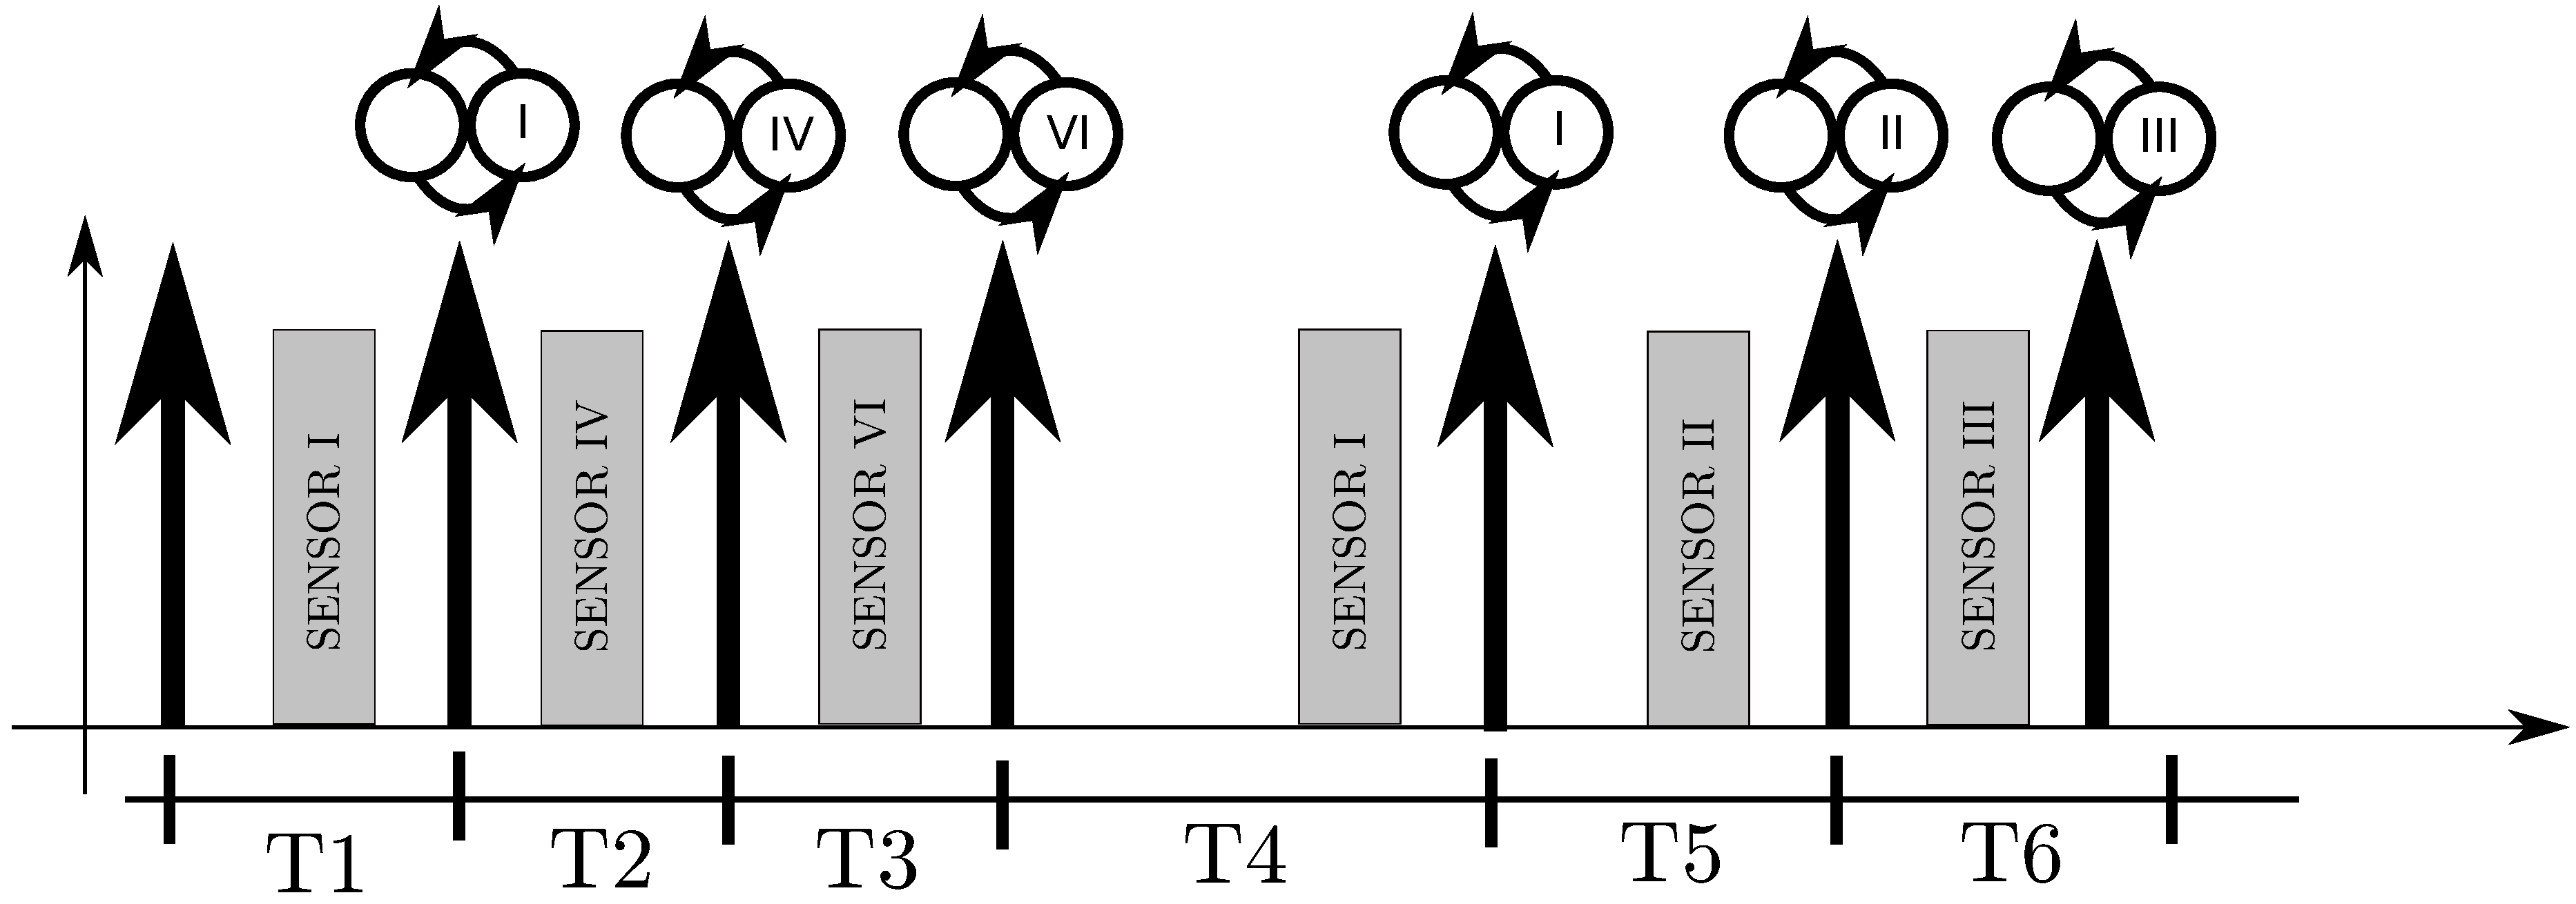
\includegraphics[width=0.7\textwidth]{methodology/fig/asynch.eps}}
    \subfigure[EKF filters periodically.]{\label{fig:synch}
    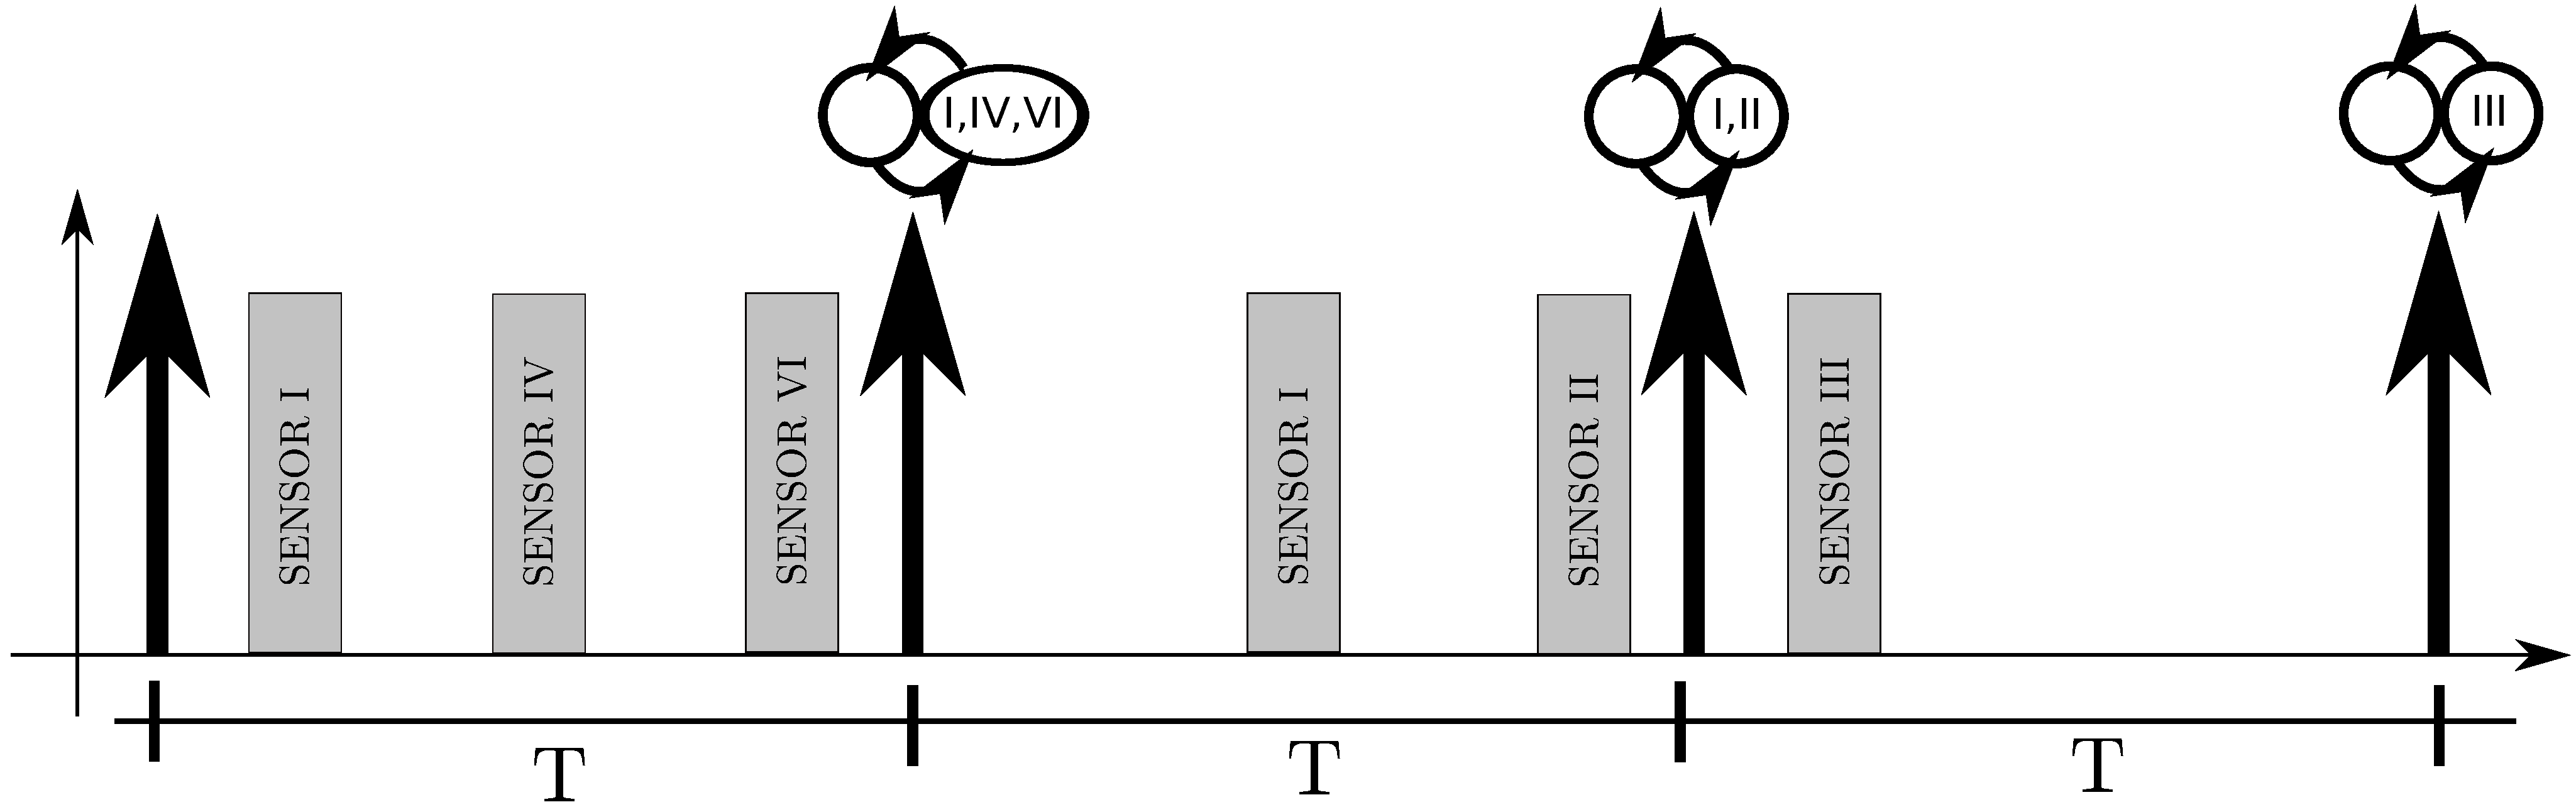
\includegraphics[width=0.7\textwidth]{methodology/fig/synch.eps}}  
  \end{center}
  \caption{Two modes for combining together sensor measurements into observation.}
  \vspace{-10pt}
  \label{fig:ekf-modes}
\end{figure}
\item \T{synchronous}
periodically updating with the most recent observation that combines together measurements from different sensors that occurred since the last update. User defined rate will determine the interval of the update.
\end{itemize}
Integrating together several different measurements into one observation would imply combining together several measurement $(\vect{Z}, \vect{H})$ and measurement noise matrices $(\vect{R})$, as shown in ~\ref{eq:concatenate-mes} for the sample case of three sensor measurements included in observation. Kalman filter maintains its own timer. Observation is reset after each timer set period.  
\begin{equation}
\label{eq:concatenate-mes} 
\vect{Z}(k) = \left[ \begin{array}{c} \vect{Z}_{sensor I} \\ \vect{Z}_{sensor II} \\ \vect{Z}_{sensor III} \end{array} \right],
\vect{H}(k) = \left[ \begin{array}{c} \vect{H}_{sensor I} \\ \vect{H}_{sensor II} \\ \vect{H}_{sensor III} \end{array} \right], 
\vect{R}(k) = \left[ \begin{array}{ccc} \vect{R}_{sensor I} & 0 & 0 \\ 0 & \vect{R}_{sensor II} & 0 \\ 0 & 0 & \vect{R}_{sensor III} \end{array} \right]
\end{equation}
Literature offers different approaches in managing Kalman filter update and managing observations. Matrix concatenation is used to gather together all the measurements into one observation. In case certain sensor measurement repeats during the update interval, the most recent measurement takes place of its preceding one within the periodic observation. This substitution is fairly realistic to happen, knowing that the user chooses filter update interval and that sensor devices have a range of frequencies, possibly more frequent that filter itself (table ~\ref{tab:sensors-char}). Simply put, observation is a buffer that stores the most recent collection of different measurements that occurred in meanwhile. Depending on the mode of operation (asynchoronous or synchrononus) the observation can contain the measurement from an individual sensor or those sensors that were active during the predefined period $T$ of update (Figure ~\ref{fig:synch}). Choosing the newest measurement is advantage from the point of having the most recent value as measurement, especially if the Kalman update interval is longer. However, it can also be a disadvantage in situations when certain sensor measurements happen at the beginning of the observation interval. For those ``earlier'' measured values, prediction stage will use less accurate time-stamp in EKF and the measurement itself would suit reality less, since it's usage is delayed. This effect is visible if update periods of EKF are long, which is not common case.  

Having more than one measurement involved in estimation of the global state is a good characteristic. The estimate which uses more diverse data gives better estimate since it is possible to combine together more that one sort of observation. Another advantage follows the fact that the whole set of state variables is updated each time, resulting in more correlation between variables. Hence those that are missing for some reason can be compensated this way. Results of simulations using authentic data and the  real misssions are given in Chapter \S~\ref{chap:results}. 
%\section{Non-linear Kalman Filter}
%By implementation standard filtering techniques such as the non-linear Kalman filtering or ``unscented'' filtering, one can obtain a minimum mean squared error estimate of the state conditioned upon all observations up to current time.
\section{Correction}
IMU is integrating acceleration or speed data collected from devices such as gyroscope or accelerometers. Integration of noisy data over time time or usage of ``relative measurements'' (those calculated from absolute measurements) results in drift or bias of the final estimate. In order to recover from that, algorithms perform correction. Correction takes an absolute measurement which should be less precise, possibly noisy, but not prone to drifting. An example which illustrates the phenomenon could be a man that walks with the eyes closed and tries to keep the track of his position by measuring the steps and predicting where he could possibly be judging on number of steps and their size. Steps have the role of ``relative measurement'' - one quantity is used to estimate the other one that's correlated with it. Naturally, a man will keep making errors in his position estimate. Moreover, these errors will accumulate over time producing drift. Correction would require man to open his eyes and observe the current position (absolute measurement), compare it with the position predicted by counting steps and neutralise the drift before carrying on with the eyes closed. 
\section{Sensor fusion}
Localisation algorithm collects the incoming sensor information and computes the pose of the vehicle by processing the whole data cluster obtained from sensor devices. Such procedure is regarded as \textit{sensor fusion}. Basic sort of sensor fusion implementation is incorporated in navigation algorithm by combining different quantities into a jointly updated state vector.
\section{Implementation} \label{sec:implementation}
Localisation algorithm was planned to be part of navigation module of Ocean System Lab's Nessie vehicle. Vehicle's real-time operating system is Linux (Unix). Designing navigation requires programming the module using C++ programming language, conforming with available libraries. The aim is to produce an applicable module that fits in the existing software system and accomplishes the task theoretically explained in this chapter. In addition, Nessie is supported with Robot Operating System (ROS, \url{http://www.ros.org/wiki/}) - meta operating system that manages various processes maintained on vehicle and the real-time exchange of data between different modules. Hence, EKF navigation is implemented as a ROS package tailored to Nessie's messaging and processing scheme. One of the difficulties that needs to be taken into account when working with angles is angle wrapping - an inevitable issue in all the implementations that involve angular values. Fact is that filtering does calculations with the angular values. Moreover, angular functions are $2\pi$ periodical. Hence, it is sufficient to represent the values in a limited interval, e.g. from $(0,2\pi]$, or $(-\pi,+\pi]$. Angle values need to be scaled back to the interval after multiplication or subtraction because the value obtained without wrapping can be misleading, especially if it expresses discrepancy or if is used for the correction. Simply, raw subtraction does not always correctly express the relation between two angles in terms of their difference and can cause unwanted behaviour. An example is shown in Figure ~\ref{fig:ang-wrapping}. Two similar angular signals (real and estimated heading value: $ang_{1}$ and $ang_{2}$, wrapped in different intervals) have been subtracted (Figure ~\ref{fig:ang-wrapping}, up). If the output of subtraction is used for control or gain, system would sense false jumps. Different intervals of angle wrapping (Figure ~\ref{fig:ang-wrapping}, down) can make difference, too. Therefore angle wrapping to $0,2\pi$ and $-\pi,+\pi$ does not give the same result. 
%%%%%\begin{figure}%[htp]
%%%%%  \begin{center}
%%%%%    \subfigure[First angular signal.]   {\label{fig:first}   
%%%%%    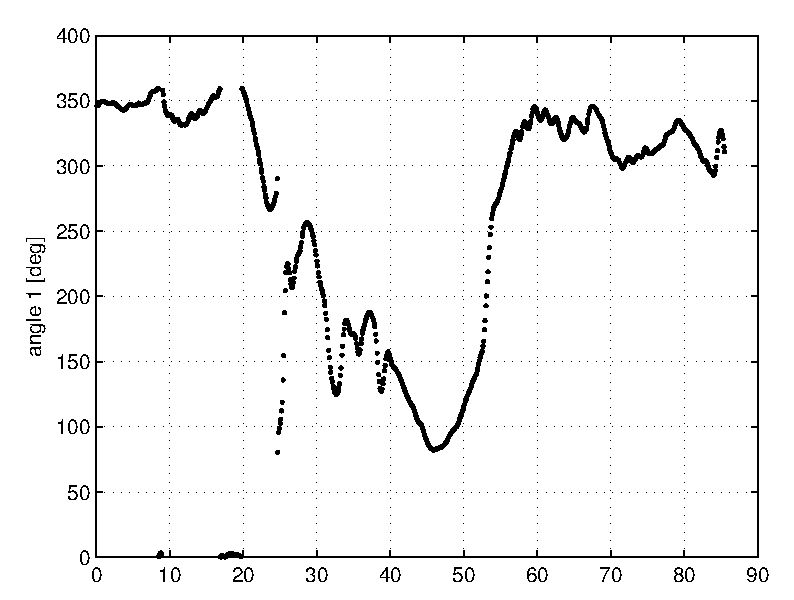
\includegraphics[width=0.42\textwidth]{methodology/fig/angle1.eps}}
%%%%%    \subfigure[Second angular signal.]{\label{fig:second}
%%%%%    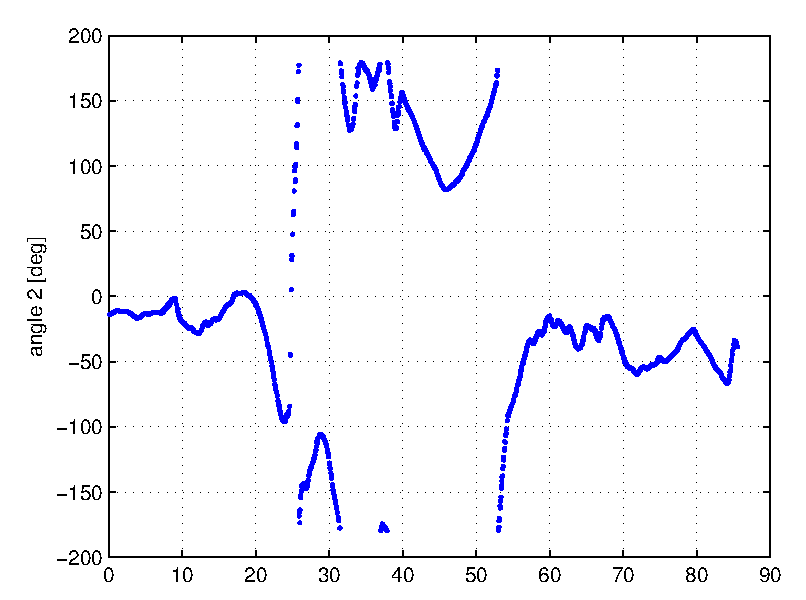
\includegraphics[width=0.42\textwidth]{methodology/fig/angle2.eps}}  \\
%%%%%    \subfigure[Difference of two signals. ]   {\label{fig:diff}   
%%%%%    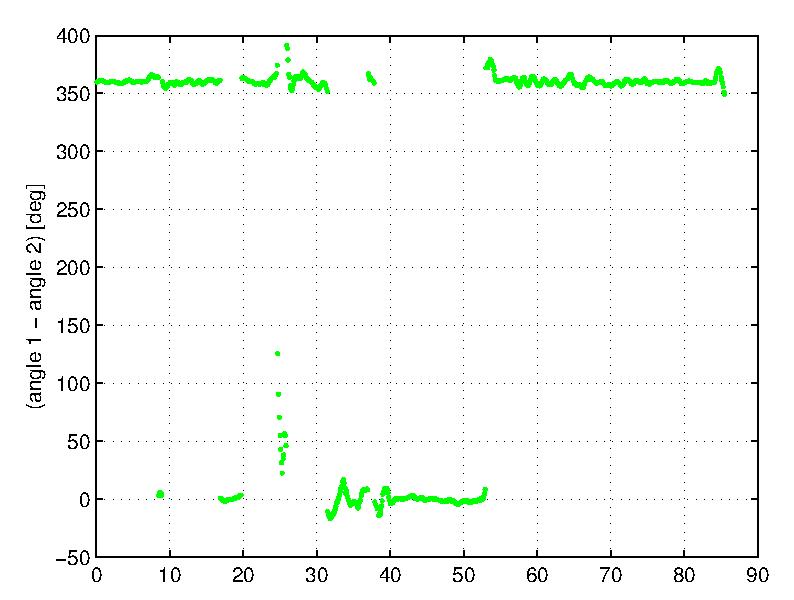
\includegraphics[width=0.42\textwidth]{methodology/fig/angle1-2.eps}}
%%%%%    \subfigure[Angle wrapping in $0/+360$ and $-180/+180$. Angular values used as gain should be wrapped around zero.]{\label{fig:diff-wrap}
%%%%%    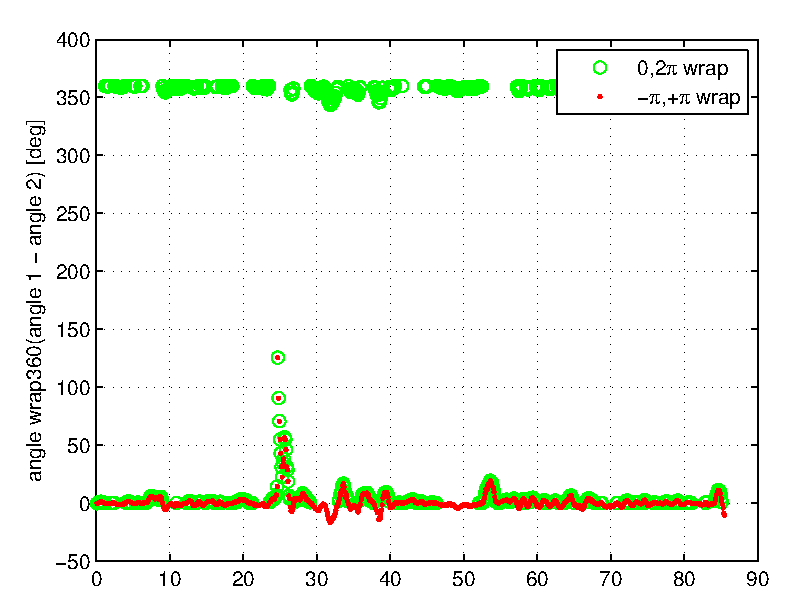
\includegraphics[width=0.42\textwidth]{methodology/fig/wrapangle1-2.eps}}   
%%%%%  \end{center}
%%%%%  \caption{}
%%%%%  \vspace{-10pt}
%%%%%  \label{fig:ang-wrapping}
%%%%%\end{figure} 

%For instance, $-4^{\circ}$ and $356^{\circ}$ are the same angle, but using each of them as some sort of a control input can cause unwanted behaviour. 
\begin{figure}[h]
\vspace{-10pt}
\begin{center}
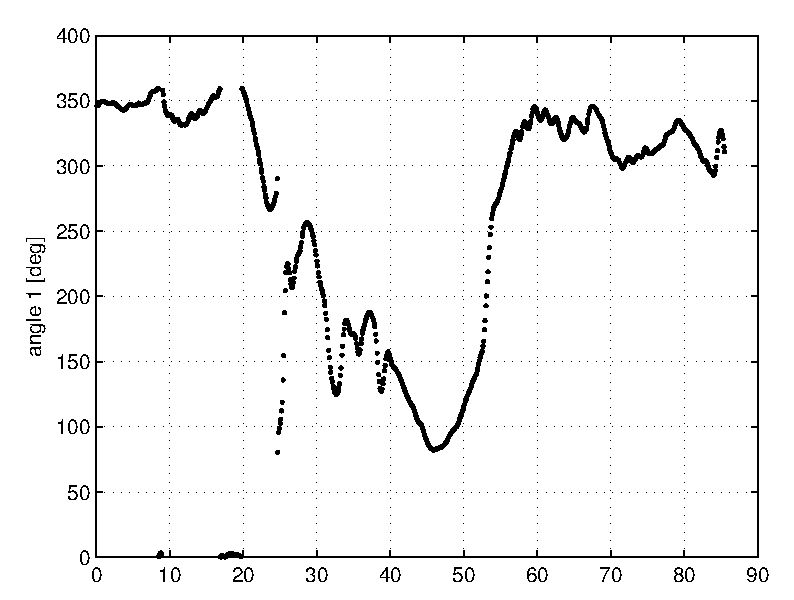
\includegraphics[width=0.45\textwidth]{methodology/fig/angle1.eps}
\caption{Importance of angle wrapping. Angular values used as gain should be wrapped around zero.}
\vspace{-10pt}
\label{fig:ang-wrapping}
\end{center}
\end{figure} 
%\chapter{Results} \label{chap:results}
Main purpose of the thesis is the implementation of a navigation system that uses measurements from different sensors, fuses the sensory data together in order to make presumably better quality estimate of the position and the orientation of the underwater robot. Existing data from the real missions were used to carry out the initial trials. It is useful to mention that there is no exact ground truth for underwater robot localization available. GPS signal, if available, could serve as an absolute position reference: either directly or in form of LBL. Experimental results have been obtained for different missions. Good news, however, is that the absolute depth measurement is quite accurate and frequent, making AUV localisation a 2D task.  

\section{Real navigation scenario} \label{sec:real-scenario}
Authentic data taken from previously recorded Nessie mission were used to simulate the algorithm ``offline'' as the part of the stage intended for testing and correcting. Besides, being able to repeat the same measurement scenario enables more insight in filtering process and benefits of fusing together the sensor data. \textit{.bag} files (\url{http://www.ros.org/wiki/}) containing recorded real-time messages with sensor measurements, were used as source. Furthermore, it allows designing the code in its original C++ form that will require little modification once deployed on the vehicle in form of ROS package since \textit{.bag} files emulate authentic messages and timestamps. One of the deficiencies of the evaluation of localisation results is the fact that there is no exact ground truth to compare the result with. Dead reckoning localisation substituted with occasional LBL position updates was compared with the localisation obtained after filtering (Figures ~\ref{fig:auv-sim-straight2}, ~\ref{fig:auv-sim-straight1}) for the recorded straight line trajectory mission. 

\T{Selecting a heading measurement with good performance}
For a high-end underwater vehicle such as Nessie, supplied with FOG-based INS, DVL and LBL, main source of navigation error is influenced by transformation of vehicle-referenced velocities to world-referenced velocities \cite{bahr08}, particularly due to yaw (heading) measurement errors. Yaw can be measured using several devices, each having different accuracy and performance. Simulation with data from previous missions was carried out to see which device gives the best performance for a given underwater vehicle. 

Heading calculated by integrating FOG's yaw rate - tends to be accurate and fast, less prone to noise. Nevertheless, it is calculated each time by appending yaw rate value integrated in time on the previous yaw value (relative measurement). Therefore, it is sensible on initial absolute heading measurement. In case initial yaw is imprecise, a constant bias exists in yaw measurement (Figure ~\ref{fig:auv-sim-straight1}). Constant bias causes sudden steps in position estimate obtained using EKF. This is expected scenario since the sensor responsible for measuring initial heading is magnetic compass, device sensitive to disturbances coming from environment (Figure ~\ref{fig:magnetic-disturb}). In real experiments biggest obstacle was proper calibration of magnetic compass. In practice, tests have showed many failures in compass heading measurement, possibly due to calibration and magnetic declination. There is yet space to do more testing with better compass tuning. To overcome the problem of accurate yaw measurement, EKF used in experiments will either ignore the yaw measurement (it is possible since sensor fusion successfully compensates missing heading information with yaw rate obtained from FOG) or use it with high variance assigned to yaw measurement. 
%Finally, initial heading is given with magnetic compass.

\T{Loch Earn dataset - straight line movement}: Example of basic EKF localisation using inertial measurements aided with LBL acoustic positioning system was tested on straight line movement of approximately 80 m length, recorded at the lake Loch Earn. For simulation purposes, sensor measurements are stored in a \textit{.bag} file, that can be replayed, producing real-time messages of sensor measurements as they originally occurred. At this point, it is important to revise which sensors were used, their main features and, finally, filtering parameters. 

Standard sensor configuration comprising of pressure sensor, magnetic compass, FOG and DVL is used in the mission. Absolute position correction was carried out using LBL system. Important fact is that the heading was measured with magnetic compass only at the beginning. Later on, it kept being calculated by integrating yaw rate obtained from FOG. Alternative solution for the heading measurement would be the usage of compass for direct acquiring of yaw, but such option exposed calibration difficulties. Result of EKF localisation algorithm was shown in north-east map (Figure ~\ref{fig:sim-straight2}, ~\ref{fig:sim-straight1}). Different parameter values for EKF were tested. Table ~\ref{tab:ekf-params} revises all filter parameters used for filter tuning, together with their role. Essentially, setting high standard deviation for a Gaussian of a certain parameter can be interpreted as having more uncertainty in value that it represents - whether it is a measurement uncertainty or uncertainty of the predicted value (model uncertainty). Therefore, we can choose to be confident in certain sensor measurement and/or certain model prediction, and observe the simulation outcome of such setting. Setting the parameters properly improves the performance of the filter.  
\addtocounter{footnote}{1}
\footnotetext[\value{footnote}]{as it appears in algorithm equations}  
\begin{table*}
\centering
	\caption{EKF navigation parameters.}
	\label{tab:ekf-params}
\begin{tabular}{llll}
\toprule
Parameter      &     Signature $^{\decimal{footnote}}$     &     Units     &    Description  \\
\midrule
                         & \multicolumn{3}{c}{standard deviation of the ... } \\ 
\multirow{1}{*}{SDNorth} & \multirow{1}{*}{$\sigma_{n}$} & \multirow{1}{*}{$m$} & \multirow{1}{*}{north observation} \\
\multirow{1}{*}{SDEast}  & \multirow{1}{*}{$\sigma_{e}$} & \multirow{1}{*}{$m$} & \multirow{1}{*}{east observation} \\
\multirow{1}{*}{SDDepth} & \multirow{1}{*}{$\sigma_{d}$} & \multirow{1}{*}{$m$} & \multirow{1}{*}{depth observation} \\
\multirow{1}{*}{SDAltitude} & \multirow{1}{*}{$\sigma_{a}$} & \multirow{1}{*}{$m$} & \multirow{1}{*}{altitude observation} \\
\multirow{1}{*}{SDu} & \multirow{1}{*}{$\sigma_{u}$} & \multirow{1}{*}{$\frac{m}{s}$} & \multirow{1}{*}{surge velocity observation} \\
\multirow{1}{*}{SDv} & \multirow{1}{*}{$\sigma_{v}$} & \multirow{1}{*}{$\frac{m}{s}$} & \multirow{1}{*}{sway velocity observation} \\
\multirow{1}{*}{SDw} & \multirow{1}{*}{$\sigma_{w}$} & \multirow{1}{*}{$\frac{m}{s}$} & \multirow{1}{*}{heave velocity observation} \\
\multirow{1}{*}{SDyaw} & \multirow{1}{*}{$\sigma_{\psi}$} & \multirow{1}{*}{$rad$} & \multirow{1}{*}{heading observation} \\
\multirow{1}{*}{SDpitch} & \multirow{1}{*}{$\sigma_{\varphi}$} & \multirow{1}{*}{$rad$} & \multirow{1}{*}{pitch observation} \\
\multirow{1}{*}{SDyawRate} & \multirow{1}{*}{$\sigma_{\dot{\psi}}$} & \multirow{1}{*}{$\frac{rad}{s}$} & \multirow{1}{*}{heading rate observation} \\
\multirow{1}{*}{SDpitchRate} & \multirow{1}{*}{$\sigma_{\dot{\varphi}}$} & \multirow{1}{*}{$\frac{rad}{s}$} & \multirow{1}{*}{pitch rate observation} \\
\midrule
                         & \multicolumn{3}{c}{standard deviation of the ... process noise} \\
\multirow{1}{*}{SDuModel} & \multirow{1}{*}{$\sigma_{\dot{u}}$}  & \multirow{1}{*}{$\frac{m}{s^{2}}$} & \multirow{1}{*}{surge acceleration} \\
\multirow{1}{*}{SDvModel} & \multirow{1}{*}{$\sigma_{\dot{v}}$}  & \multirow{1}{*}{$\frac{m}{s^{2}}$} & \multirow{1}{*}{sway acceleration} \\
\multirow{1}{*}{SDwModel} & \multirow{1}{*}{$\sigma_{\dot{w}}$}  & \multirow{1}{*}{$\frac{m}{s^{2}}$} & \multirow{1}{*}{heave acceleration} \\
\multirow{1}{*}{SDyawRateModel} & \multirow{1}{*}{$\sigma_{\dot{v}}$}  & \multirow{1}{*}{$\frac{rad}{s^{2}}$} & \multirow{1}{*}{yaw acceleration} \\
\multirow{1}{*}{SDpitchRateModel} & \multirow{1}{*}{$\sigma_{\dot{w}}$}  & \multirow{1}{*}{$\frac{rad}{s^{2}}$} & \multirow{1}{*}{pitch acceleration} \\
\bottomrule
\end{tabular} 
\end{table*}
Straight line movement with authentic sensor measurements recorded in Loch Earn was a basis for initial tests of the EKF localisation algorithm. Red line shows the dead reckoning navigation, which is directly updated with absolute position update (LBL). Dead reckoning uses values periodically ($\approx$5$Hz$) obtained from DVL and FOG (linear velocities: $u$ and $v$ and heading $\psi$, respectfully), and substitutes them into equations similar to ones used for north and east prediction within prediction model: 
$$ north = north + (uT+\dot{u}\frac{T^{2}}{2})\cos(\psi) - (vT+\dot{v}\frac{T^{2}}{2})\sin(\psi) $$
$$ east  = east  + (uT+\dot{u}\frac{T^{2}}{2})\sin(\psi) + (vT+\dot{v}\frac{T^{2}}{2})\cos(\psi) $$
% SDnorth/east = 5 $cm$, 
% SDnorth/east = 5 $cm$, 
\begin{figure}%[htb]
  \centering
    \subfigure[N/E localisation. Yaw was calculated by integrating yaw rate periodically measured using FOG.] {\label{fig:sim-straight2}
	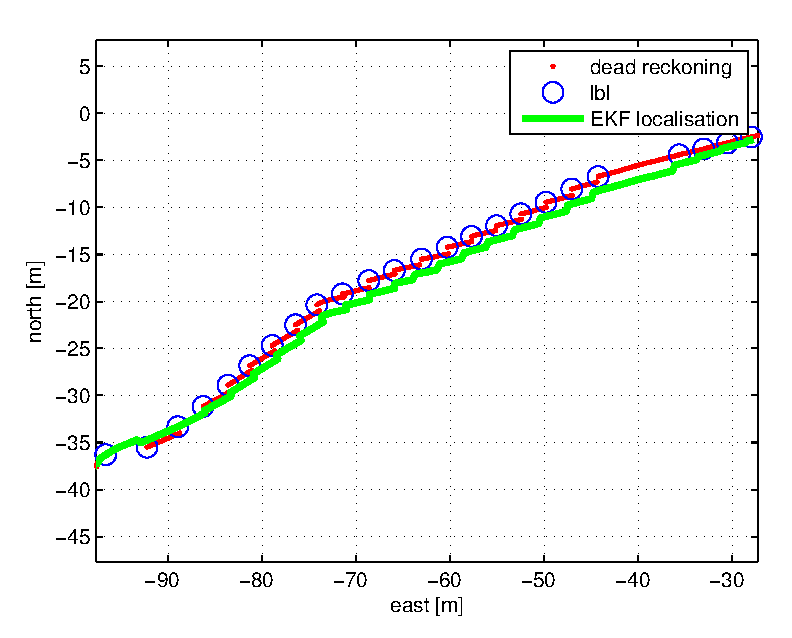
\includegraphics[width=0.48\linewidth]{simulations/fig/sim-straight2.eps}}
    \subfigure[Heading estimation. Biased yaw measurement not being corrected due to high confidence in yaw measurement.] {\label{fig:yaw-straight2}
    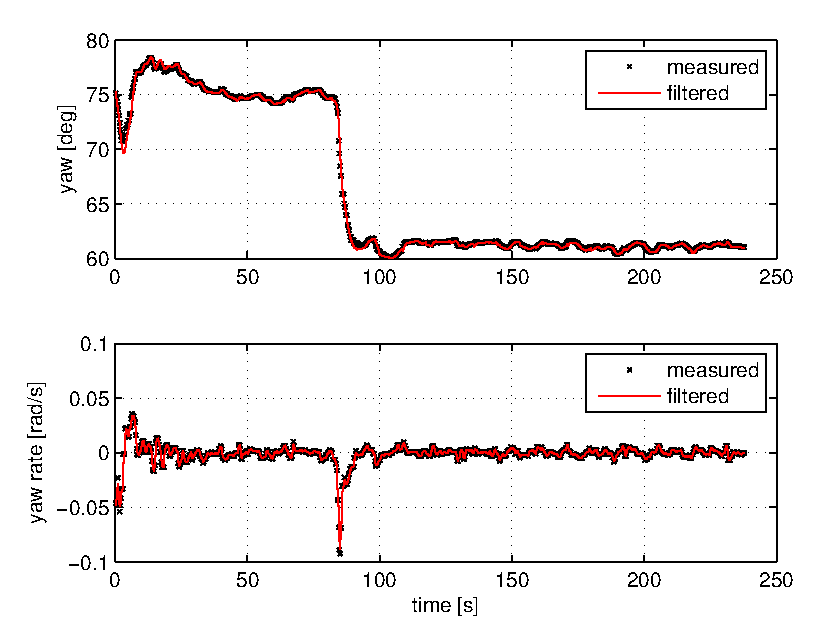
\includegraphics[width=0.48\linewidth]{simulations/fig/yaw-straight2.eps}} \\   
\caption{AUV localisation using EKF with high confidence in yaw measurement, SDyaw = 0.01$rad \approx 0.6 ^{\circ}$. SDyawRate = 0.004 $\frac{rad}{s}$, SDu/v = $1\frac{cm}{s}$.}

\label{fig:auv-sim-straight2}
\end{figure}
\begin{figure}%[htb]
  \centering
    \subfigure[N/E localisation. Yaw was calculated by integrating yaw rate periodically measured using FOG.] {\label{fig:sim-straight1}
	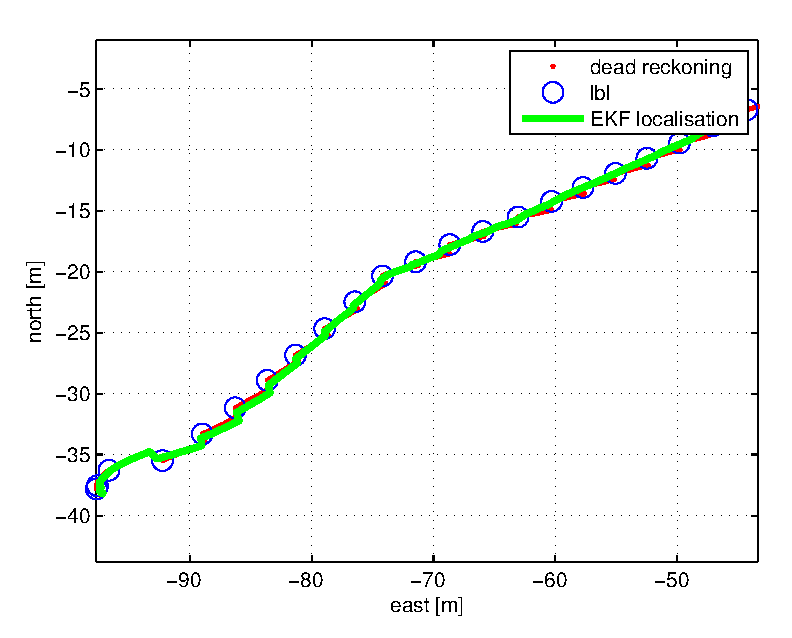
\includegraphics[width=0.48\linewidth]{simulations/fig/sim-straight1.eps}}
    \subfigure[Heading estimation. Biased yaw measurement is being corrected.] {\label{fig:yaw-straight1}
    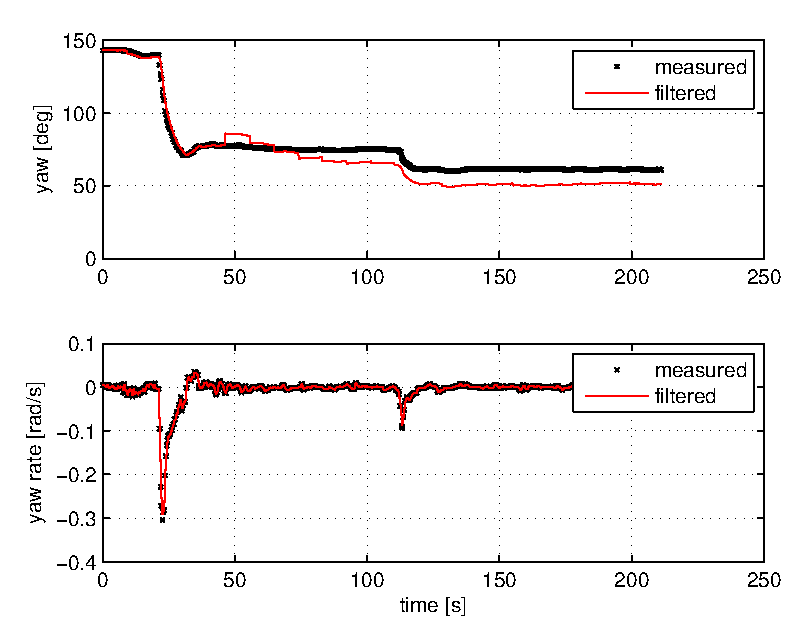
\includegraphics[width=0.48\linewidth]{simulations/fig/yaw-straight1.eps}} \\
\caption{AUV localisation using EKF with low confidence in yaw measurement, SDyaw = 0.2$rad \approx 11.5 ^{\circ}$. SDyawRate = 0.004 $\frac{rad}{s}$, SDu/v = $1\frac{cm}{s}$.}
%\vspace{-10pt}
\label{fig:auv-sim-straight1}
\end{figure}    
%After  initial heading, yaw rate was integrated in time to calculate yaw.    when setting  EKF parameter uncertainty  when using EKF, this time
EKF updates periodically (synchronous mode), with period set to 230 ms. At first, simulation parameters \textit{SDnorth}, \textit{SDeast}, \textit{SDyaw} and \textit{SDyawRate} were set to low values - suggesting high trust in measurements. Resulting trajectory (Figure ~\ref{fig:sim-straight2}) shows that the heading measurement has a constant bias, caused by the error in initial heading measurement obtained by compass. Thus, yaw measurement, calculated relative to previous value each time, propagates the error (bias). Biased yaw observation further on causes EKF localisation to experience sharp jumps. To overcome this using EKF framework, less confidence was assigned to the yaw measurement (\textit{SDyaw}) value. Eventually, bias becomes visible if measured and filtered heading are compared (Figure ~\ref{fig:yaw-straight1}). As for the rest of the heading information, rate of yaw measurement will be incorporated with a lot of confidence (\textit{SDyawRate} parameter having range of degrees) since it is a reliable device and it does not depend on the initial estimate. Good feature of sensor fusion is that lack of one measurement or its low performance can be compensated with some other measurement considering that they are combined together in mathematical model in the right manner. In case of yaw and yaw rate - the derivation in time is a relation that connects them together. 

Simulation shows that localisation performance can be tailored by setting the confidence in prediction model or measurement values. Confidence is materialized as standard deviation (variance) of the random variable: the lower it is, more certain the value of the random variable is hence more confident in value of that variable we tend to be. Kalman filter tries to optimise the result within the defined boundaries of uncertainty. 

Unscented Kalman filter was mentioned in Section \S~\ref{sec:ukf} as a good alternative in handling nonlinearities. UKF was implemented in MATLAB for the simulation purposes and its result compared with the EKF localisation, under same parameter settings and using the real data obtained from Nessie sensors. Test mission consisted of pipe tracking where the vehicle was guided along the underwater pipe three times and each time returned back to the initial position (Figure ~\ref{fig:ekf-ukf}). 2D north-east maps were compared, together with dead reckoning, same as one used for previous simulations. General characteristics of UKF are visible from the obtained shape of the UKF path (Figure ~\ref{fig:ekf-ukf}). Eventually, both filtered paths end up in approximately same position, having less drift than the dead reckoning. EKF does first order approximations, therefore, its path is slightly distorted compared with the UKF one, which was obtained with the same amount of calculation, and the inherited approximation of at least second order \cite{julier96}. Simultaneously with filtering, UKF preserves the nonlinearity formula of prediction model better - its curves have shape closer to equation-based dead reckoning curves. Still, a question that is yet opened is whether we need to improve the approximation of the prediction model. Answering this question is a hard task without knowing the movement of the object and how much it actually matches the state prediction model. A difficulty with UKF implementation is that it involves calculation of covariance matrix square root which is a slightly more complex problem, solved with numerical methods. Nevertheless, it is possible that covariance matrix becomes singular which also depends on parameter $k$ used for scaling (Section \S~\ref{sec:ukf}). $k$ was set to -0.5 for simulations shown.        
\begin{figure}%[htb]
  \centering
    \subfigure[N/E localisation. Comparison of the EKF and UKF.] {\label{fig:ekf-ukf}
	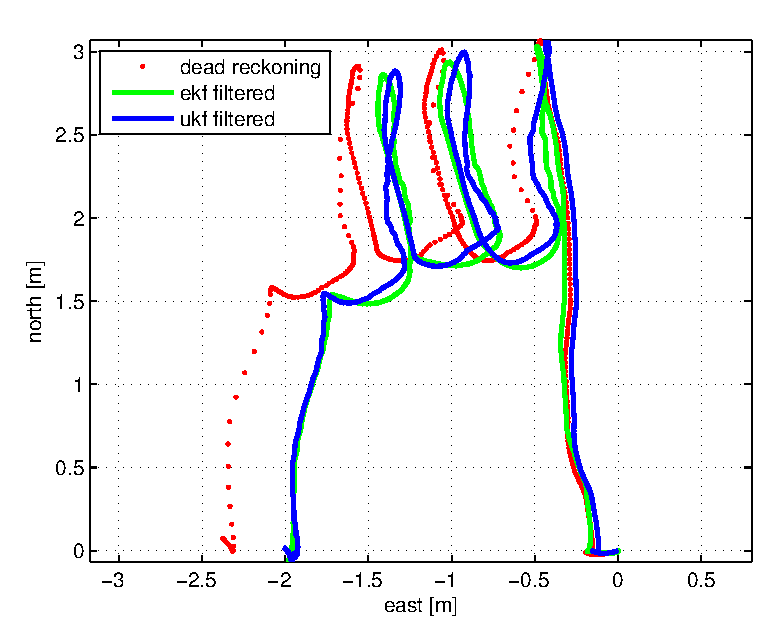
\includegraphics[width=0.42\linewidth]{simulations/fig/UKFpipeTrack.eps}}
    \subfigure[Magnetic disturbances affecting the heading measurement by compass. Vehicle is not moving, FOG is not oscillating at the same time.] {\label{fig:magnetic-disturb}
    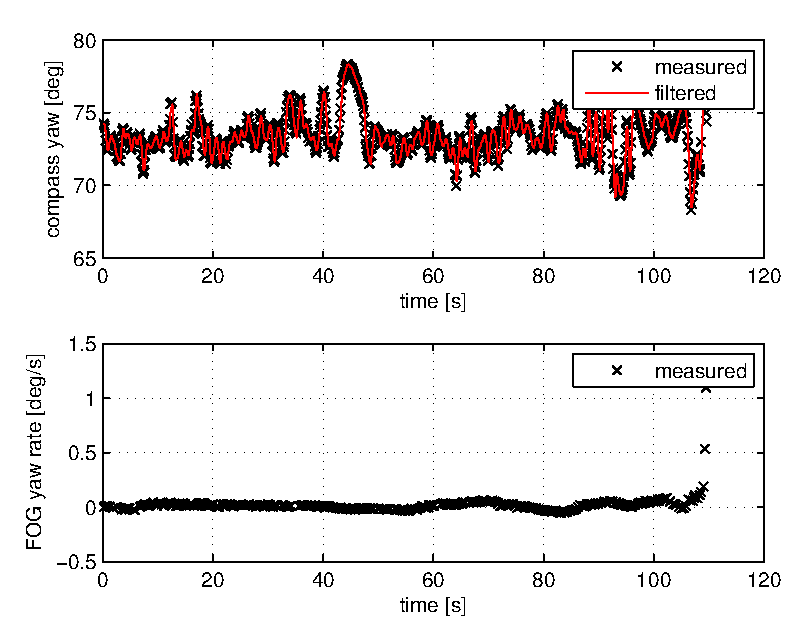
\includegraphics[width=0.42\linewidth]{simulations/fig/magnetic.eps}} 
%\vspace{-33pt}  
\end{figure}

\T{Sensor fusion for heading: } being in search for heading measurement less prone to initial error, and guided by simulation results, real scenarios were accomplished using magnetic compass for heading measurement. Compass is more sensitive to magnetic disturbances (Figure ~\ref{fig:magnetic-disturb}), slower than FOG but, importantly, gives an absolute measure. Therefore, it does not rely on previous measurements. An experiment was made by just manually rotating the robot horizontally while keeping the same position - changing its heading. Figures ~\ref{fig:lostFog} and ~\ref{fig:lostCompass} show the performance of yaw filtering using EKF and the example of sensor fusion of compass and FOG. Namely, compass (Figure ~\ref{fig:lostCompass}) or FOG (Figure ~\ref{fig:lostFog}) were disabled at one point during the experiment. When one of them stops working, the other one tries to compensate the failure. 
%and still filters the heading/yaw rate variation.  
\begin{figure}%[htb]
  \centering
    \subfigure[Compass disabled.] {\label{fig:lostCompass}
	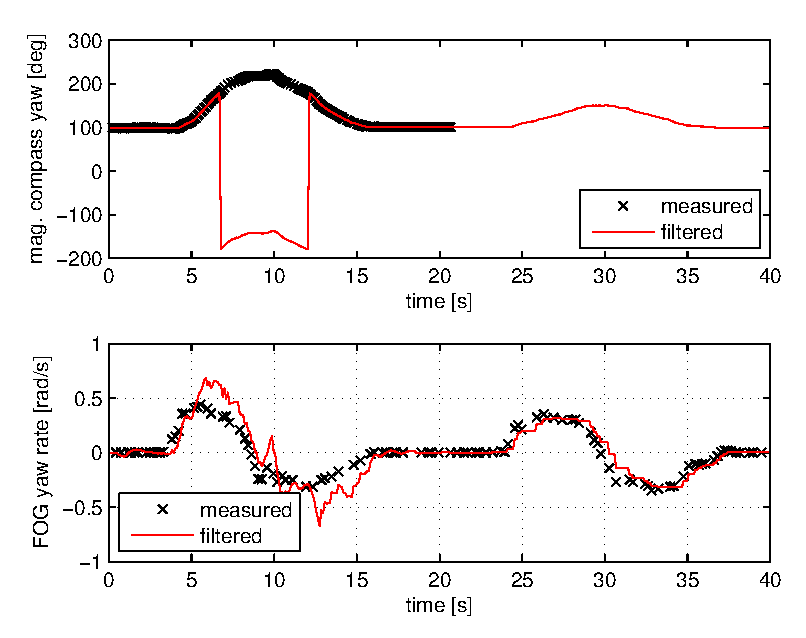
\includegraphics[width=0.45\linewidth]{results/fig/lostCompass.eps}}
    \subfigure[FOG disabled.] {\label{fig:lostFog}
    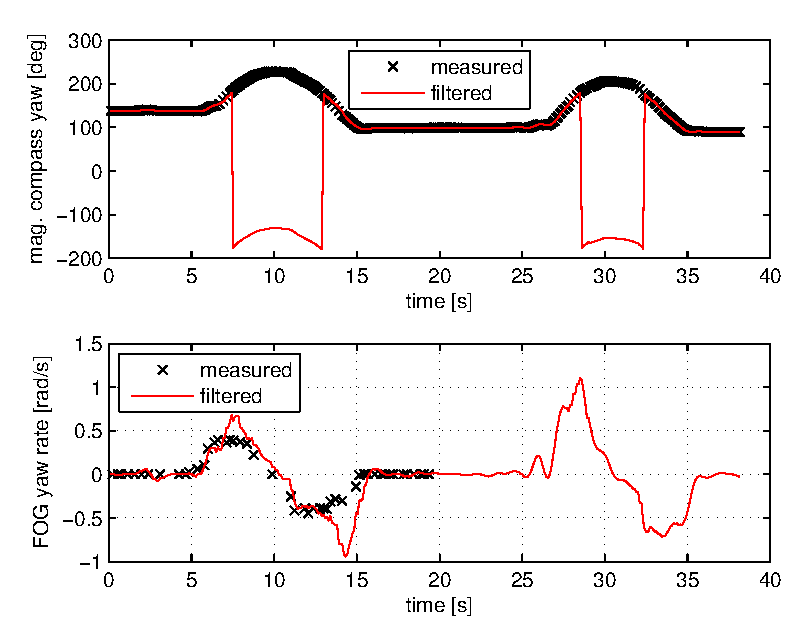
\includegraphics[width=0.45\linewidth]{results/fig/lostFOG.eps}} \\   
\end{figure}

\T{Trajectory filtering: } Spiral trajectory and surfacing action was taken with Nessie starting from the depth of around 12 m. EKF filtering results are shown in Figure ~\ref{fig:spiral} together with LBL position updates and dead reckoning starting from each position. Similarly as with previous plots, dead reckoning was shown together with LBL position updates. Filtered trajectory does not experience severe jumps, and the curve seems to be smoother and less prone to drifting. Standard deviation of north and east measurement parameter (Table ~\ref{tab:ekf-params}) was tested with different values, causing more or less confidence in LBL measurement hence shaping the filtered localisation curve. Presented LBL measurements are exhibiting quite diverse range of values.

Causes of position correction errors are numerous: from ``multipathing'' outliers (Figure ~\ref{fig:multipathing}) till the imprecision inferred from the nature of volatile acoustic and GPS information. ``Multipathing'' causes outliers in position information as a result of false reflections for instance. Acoustic and GPS imprecision can be treated as Gaussian random variable. 
\begin{wrapfigure}{r}{0.55\textwidth}
\vspace{-10pt}
  \centering
    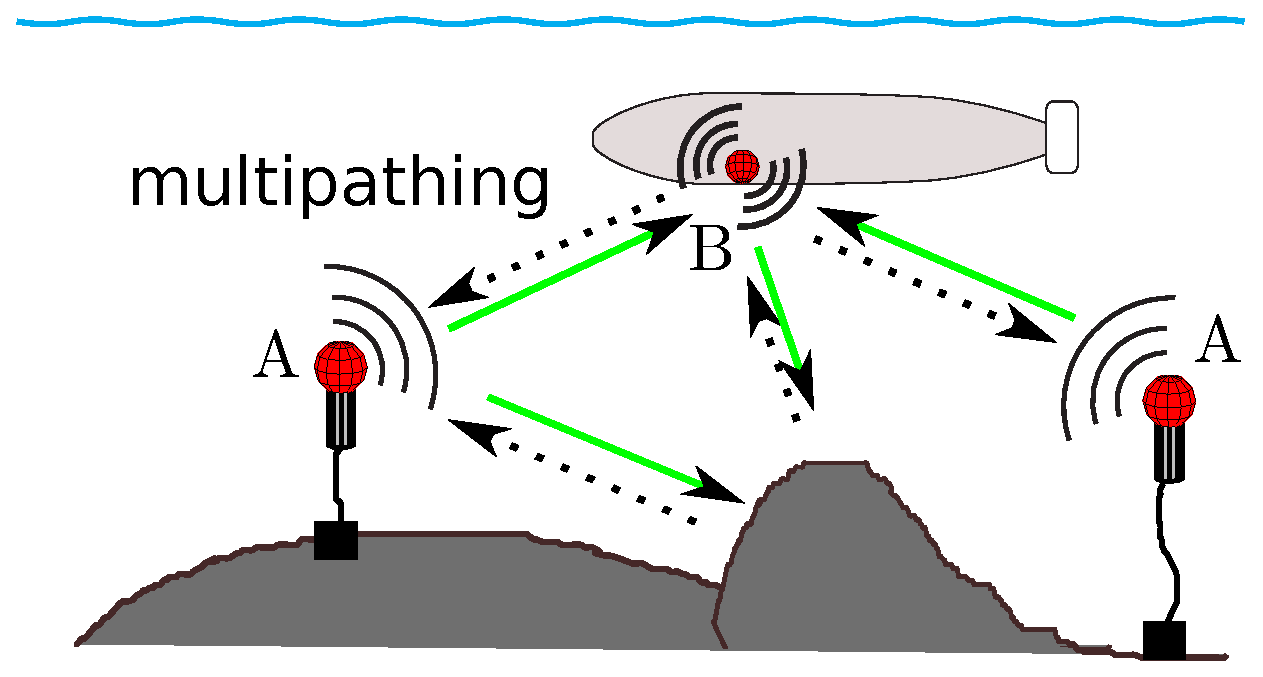
\includegraphics[width=0.45\textwidth]{results/fig/multipathing.eps}
  \caption{Multipathing can cause outliers in LBL position measurement. Due to reflection, several distances are detected, some  being false measurements.}
%\vspace{-10pt} 
\label{fig:multipathing}
\end{wrapfigure}
It is likely that some of the LBL position updates deviate from the trajectory. Hence, a mechanism for rejecting the outliers was investigated. EKF was tested on raw LBL position updates. Intention is to manage the filtration of the ``outliers'' by using properly tuned EKF. Motivation to explore such possibility comes from two scenarios encountered in earlier missions. In such missions position wad dead reckoned and LBL was used to assign each time a new value of north and east coordinate. LBL outliers were ruled out using a median filter applied on the last eleven position coordinates once the latest LBL exceeded the set threshold in position change. The missions showcased situations when: 
\begin{itemize}
\item LBL rejection is carried out despite being a ``false alarm'' - Figure ~\ref{fig:straight-median-ekf},
\item rejection of the LBL is the right choice - Figure ~\ref{fig:spiral-median-ekf}
\end{itemize}
It is important to say that LBL position filtering was implemented in form of median filter. EKF was updated with raw LBL data instead of median filter. Rejecting an LBL measurement can turn out to be right (Figure ~\ref{fig:spiral-median-ekf}) as well as a wrong decision (Figure ~\ref{fig:straight-median-ekf}). That is why EKF was suggested as an alternative. Examples of EKF's performance are shown in both Figures ~\ref{fig:straight-median-ekf} and ~\ref{fig:spiral-median-ekf}. Solution is not as categoric as median filter. Moreover, it is more robust. By giving certain trust in LBL observation it always takes it into account. Median filter, on the other hand, can be too selective in being right or wrong. If it turns out that LBL positions do follow each other, EKF continues slowly following that direction. If the outliers are isolated, EKF successfully rules them out (Figure ~\ref{fig:spiral-median-ekf}). 
\begin{figure}%[htb]
  \centering
    \subfigure[Straight trajectory: LBL outliers erroneously rejected (red). EKF tends to recover the navigation (green).] {\label{fig:straight-median-ekf}
	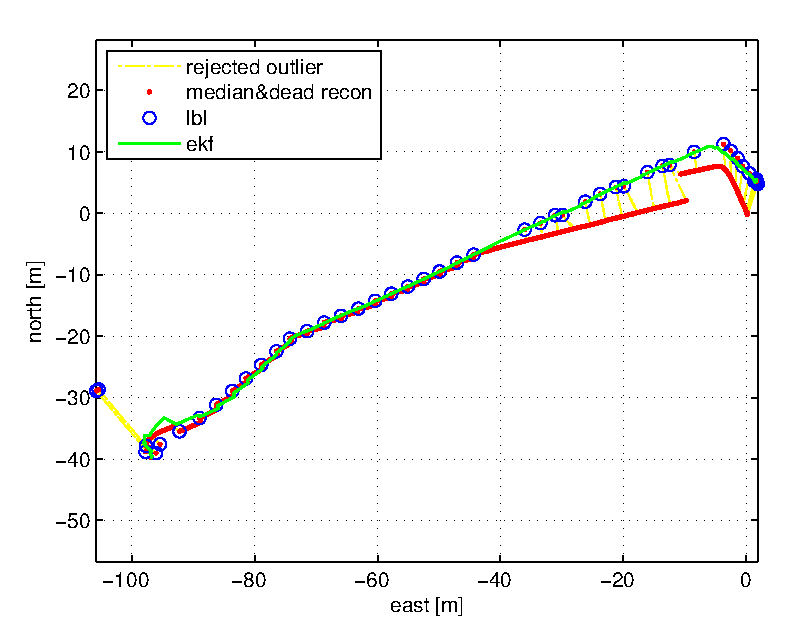
\includegraphics[width=0.47\linewidth]{results/fig/straight-median-ekf.eps}}
    %\subfigure[Straight trajectory: LBL outliers filtered with EKF.] {\label{fig:straight-ekf}
    %\includegraphics[width=0.45\linewidth]{results/fig/straight-ekf.eps}} \\  
    \subfigure[Spiral trajectory: LBL outliers are rejected using median. EKF filtering introduces the position disturbance which recovers soon after.] {\label{fig:spiral-median-ekf}
    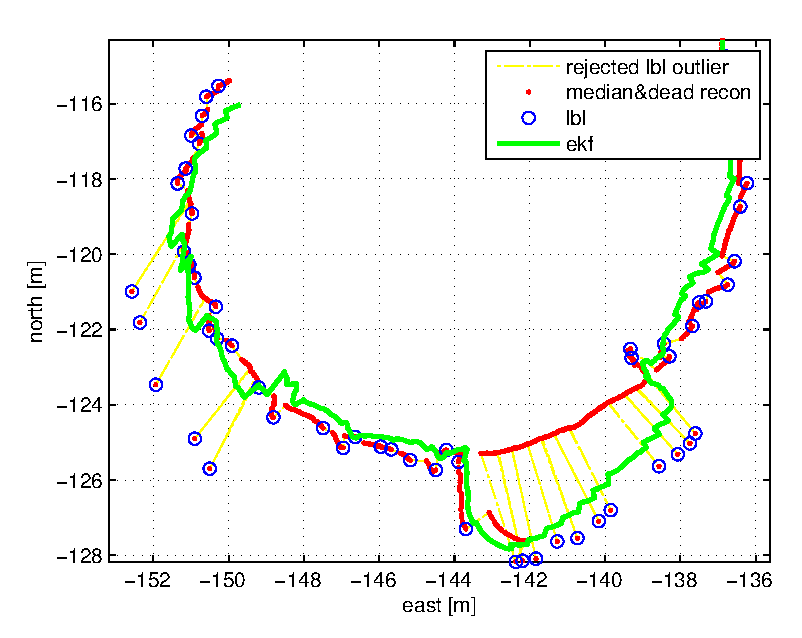
\includegraphics[width=0.5\linewidth]{results/fig/spiral-median-ekf.eps}} 
    %\subfigure[Spiral trajectory: LBL outliers filtered with EKF.] {\label{fig:spiral-ekf}
    %\includegraphics[width=0.45\linewidth]{results/fig/spiral-ekf.eps}}     
\end{figure}

\T{Square trajectories: } square trajectories were tested in low depths of a lake, with the GPS signal available to be used as a position reference and ground truth indication (Figures ~\ref{fig:no-gps}, ~\ref{fig:with-gps}). Dead reckoning navigation was used as a reference when controlling the vehicle movement during the experiment. This fact can cause slight confusion in analysis of the trajectory graphs since all the dynamics and forces were applied with respect to the dead reckoning navigation which is an estimated value, not the real existing one. It is a slightly inverse logic of testing, nevertheless further tests are yet to be accomplished. Emphasis of this experiment was to show that EKF can work successfully and analyse the main characteristics of the navigation design. It is likely that the GPS emulated square-shaped trajectories float as the elapsed path becomes longer. GPS signal available from the antenna located on the water surface is serving as a measure of absolute position within the lake - giving an idea about the actual vehicle position while it tries to moves within the boundaries of estimated dead reckoning position. 

Main issue when performing the square trajectory tests was significant imprecision of GPS signal. Many reasons can possibly influence the imprecision: from the weather conditions till surrounding objects. Basically anything that can affect the satellite visibility and the quality of the signal. Drifting can reach up to several meters which is unacceptable considering the trajectory length. Finally, the trajectory of the experiment itself is quite short ($ \approx 10 m $) to be seriously and accurately covered with precise GPS position update. Figure ~\ref{fig:gps} shows the tested trajectory and depicts the encountered amount of GPS imprecision.
\begin{figure}%[htb]
  \centering
    \subfigure[Coordinates of the tested square trajectory pasted on the lake map.] {\label{fig:gps-map}
	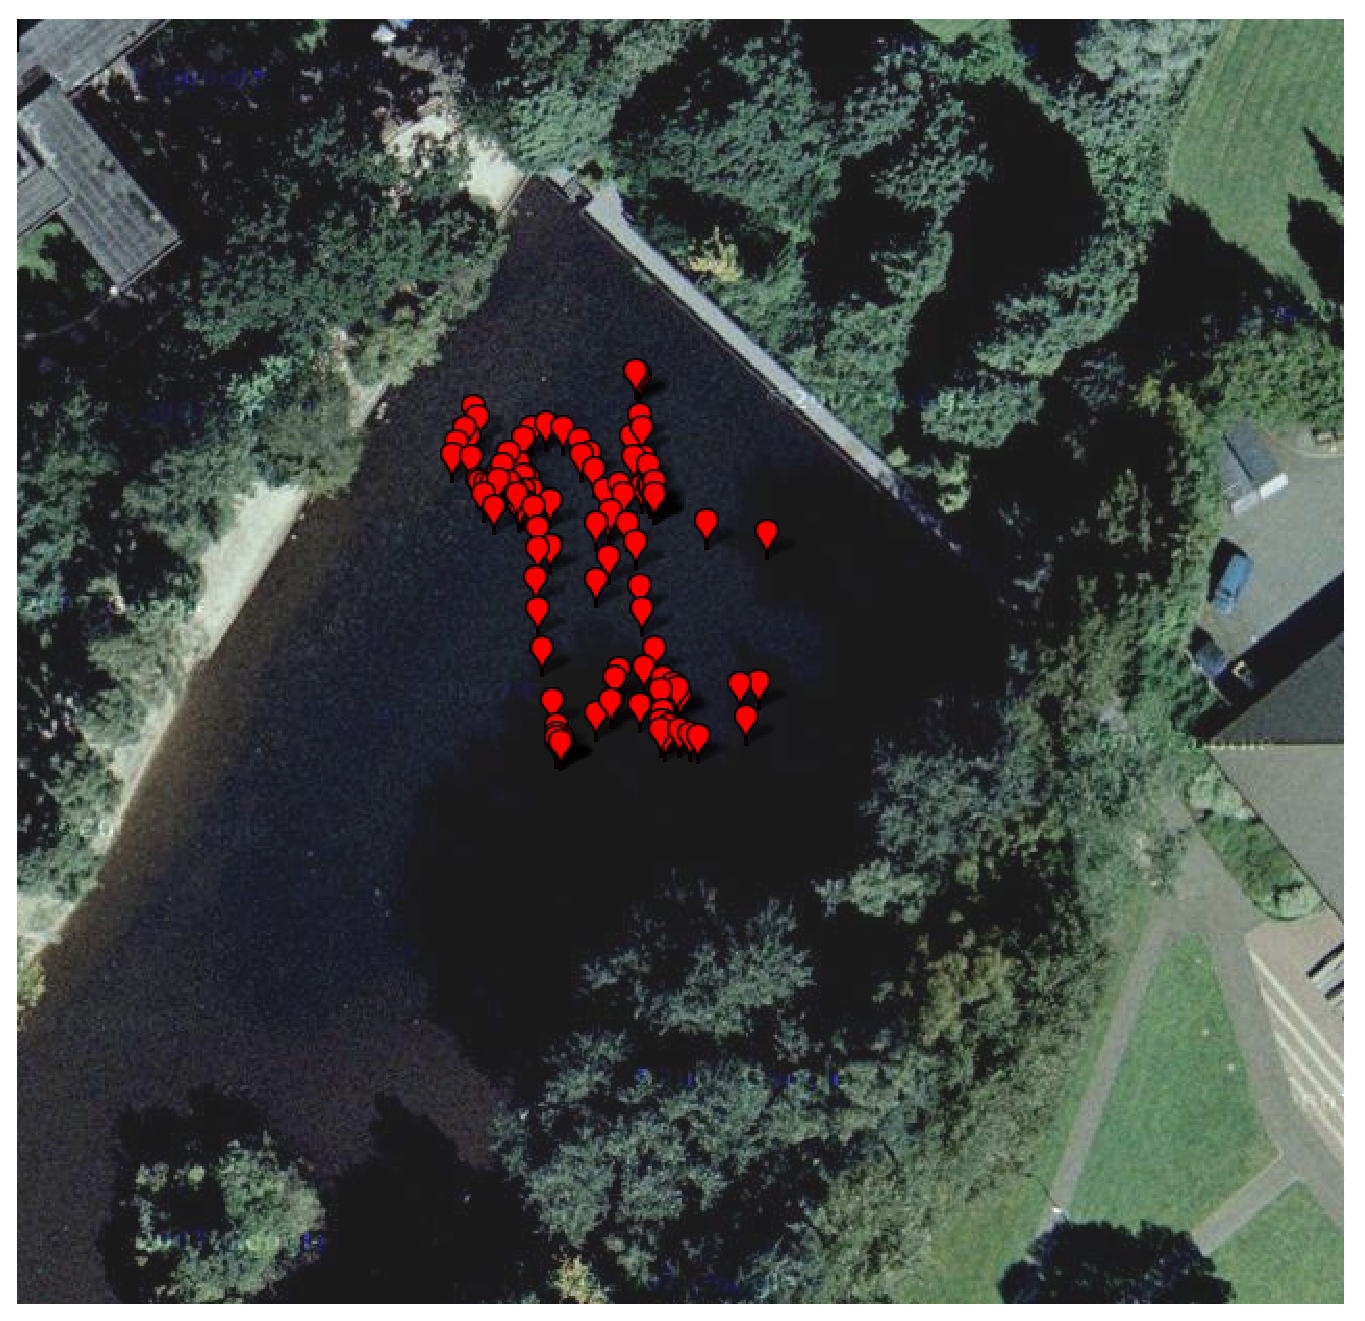
\includegraphics[width=0.48\linewidth]{results/fig/square-trajectory.eps}}
    \subfigure[GPS signal as it appears originally.] {\label{fig:gps-signal}
	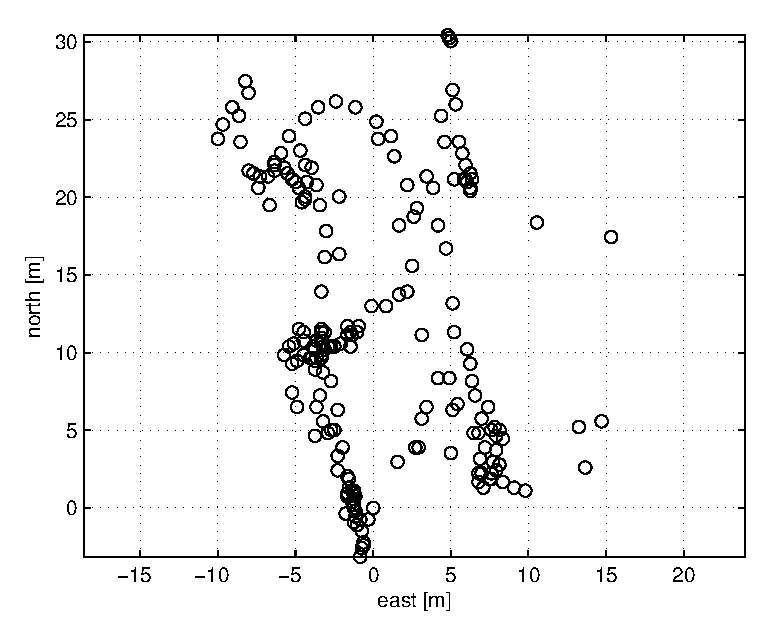
\includegraphics[width=0.48\linewidth]{results/fig/gps-signal.eps}}
\end{figure}

\T{Without GPS: } EKF localisation was tested in given conditions. Initially, only motion (inertial) sensors were used within the observations. That implies all the available linear and angular velocity sensors. Absolute position (raw GPS signal in this constellation) was not included in observations. EKF periodically updates (synchronous mode, \S~\ref{chap:methodology}), with the rate of 10 Hz. The aim was to measure the performance and the amount of drifting that occurs since the robot is intended to repeatedly attain square-like paths and return to the starting position in ideal scenario. It is useful to mention that proper parameter tuning can significantly change filtering performance. By giving more or less trust in particular measurement, or particular model behaviour, the role of certain parameters of dynamics (velocities, angular velocities) can be emphasized if necessary. Figure ~\ref{fig:no-gps} shows the performance of EKF without GPS position correction after one trajectory cycle, and the original path that was followed, recorded using GPS. Initial position was taken from the first GPS measurement and the first measurement can indeed be away from the real position due to GPS imprecision. Note that the control of the vehicle trajectory refers to dead-reckoning calculated north-east values, not some physical beacons with known position. At the time of reporting the experiments, testing were not fully completed with all the planned scenario variations. Localisation expectedly tends to perform with a significant drift without the absolute position update (Figure ~\ref{fig:square-1-noGps}). After the second square-shaped cycle (Figure ~\ref{fig:square-2-noGps}), EKF shows that it roughly tracks the shape of the trajectory, smooths it by filtering out the measurement outliers. Vehicle has returned approximately to the same position after each cycle. Drift gained when following one of the sides of the rectangular path was compensated with the same amount of drift but of the opposite sign that was active when taking the return direction. Enormous amount of drift is present since the information on absolute position is not considered. The first available GPS coordinate fixes the starting position and part of the initial position error is caused by being incapable of setting the initial position accurately.       
\begin{figure}%[htb]
  \centering
    \subfigure[N/E localisation.] {\label{fig:spiral2d}
	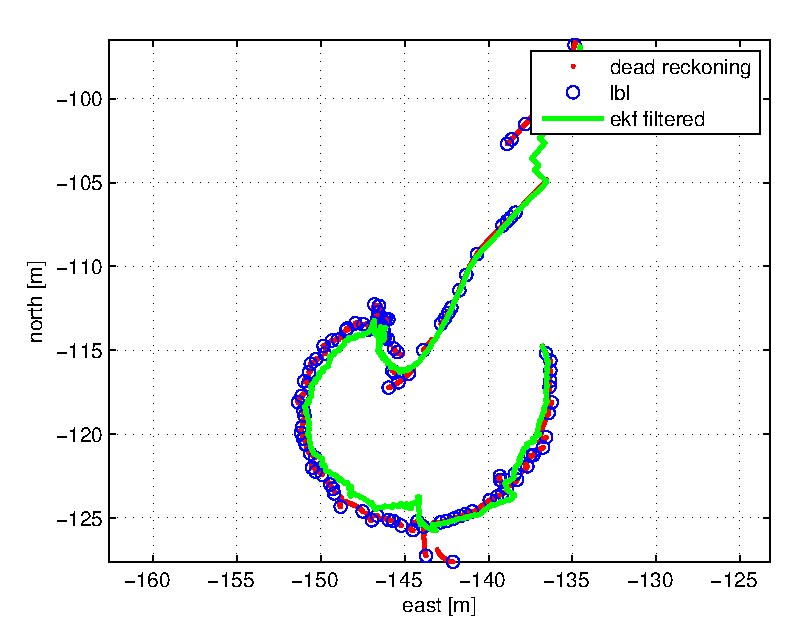
\includegraphics[width=0.48\linewidth]{results/fig/spiral2d.eps}}
    \subfigure[Depth.] {\label{fig:spiral-depth}
    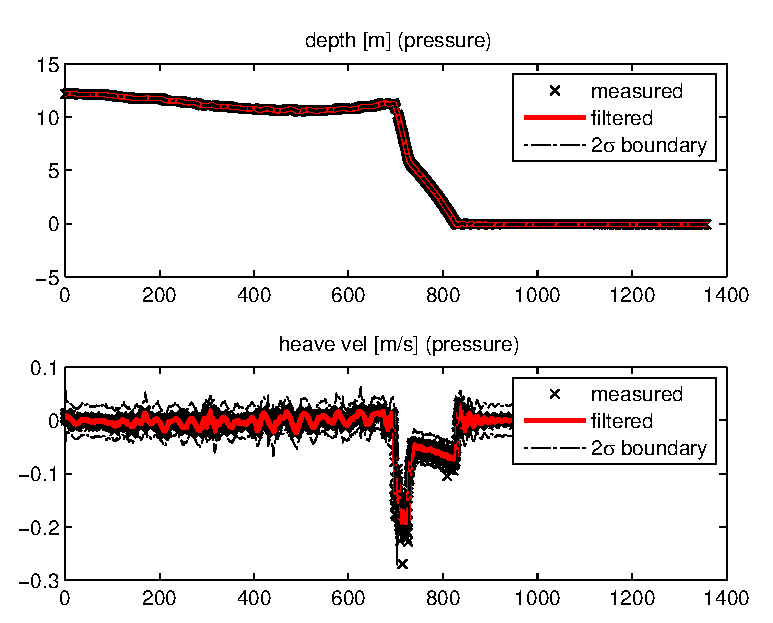
\includegraphics[width=0.48\linewidth]{results/fig/spiral-depth.eps}}
    % \\  
    %\subfigure[Path (temporary plot).] {\label{fig:spiral3d}
    %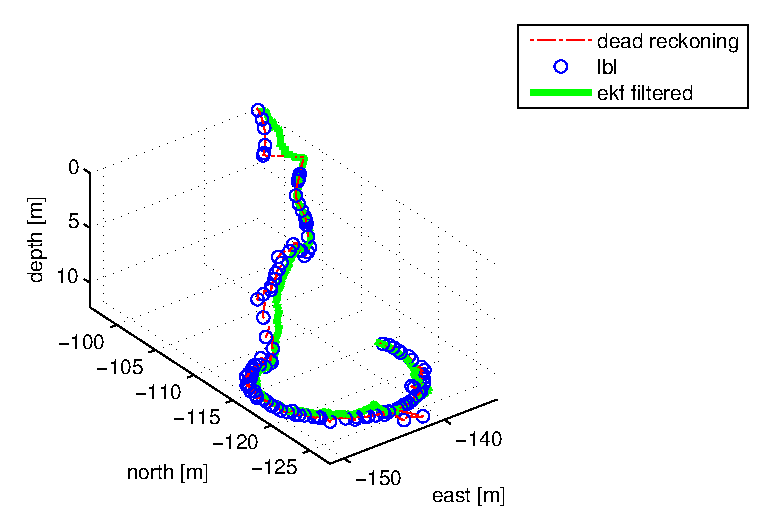
\includegraphics[width=0.8\linewidth]{results/fig/spiral3d.eps}} 
\end{figure}
\begin{figure}%[h]
  \centering
    \subfigure[EKF localisation after one cycle.] {\label{fig:square-1-noGps}
	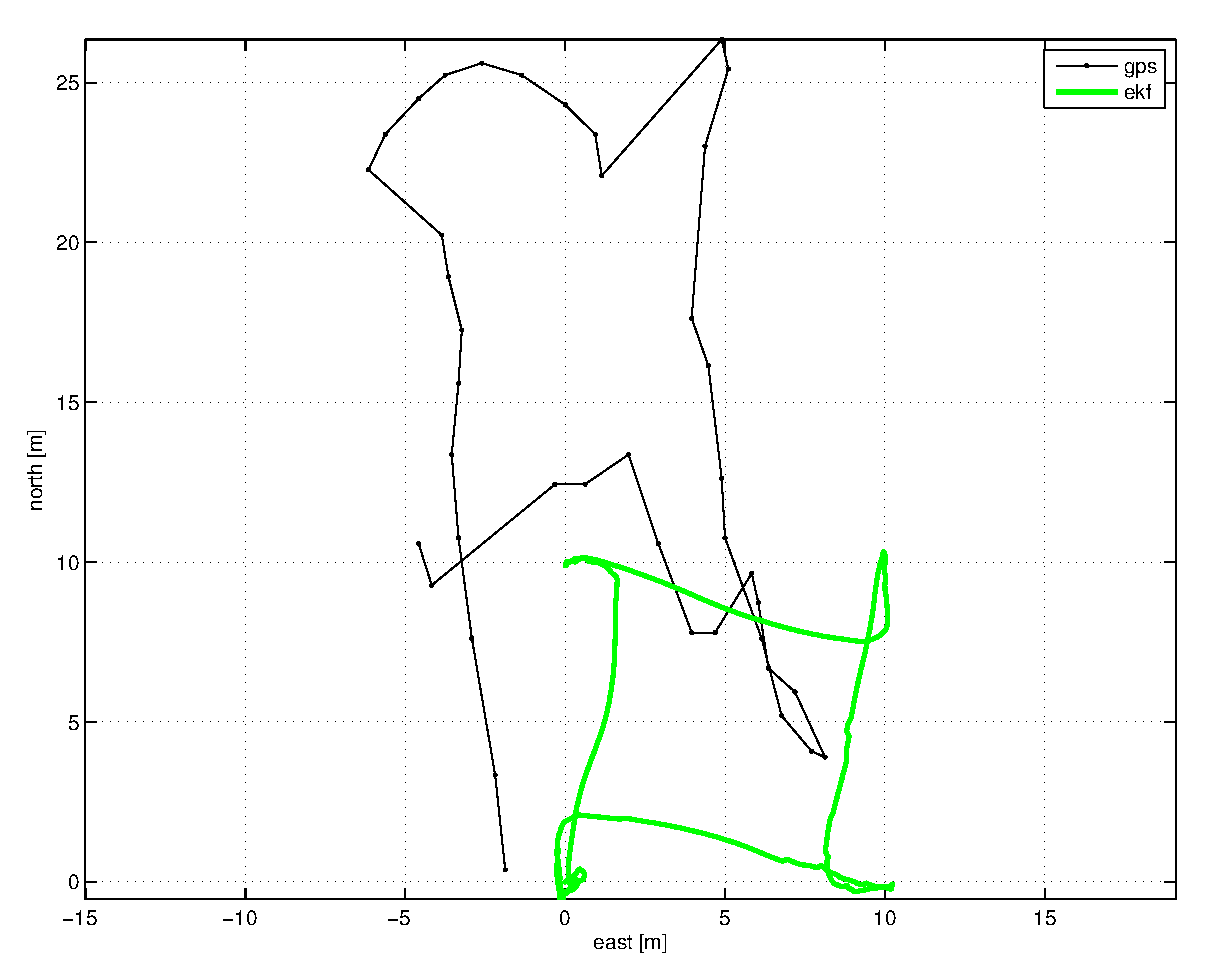
\includegraphics[width=0.48\linewidth]{results/fig/square1NoGps.eps}}
    \subfigure[EKF localisation after two cycles.] {\label{fig:square-2-noGps}
	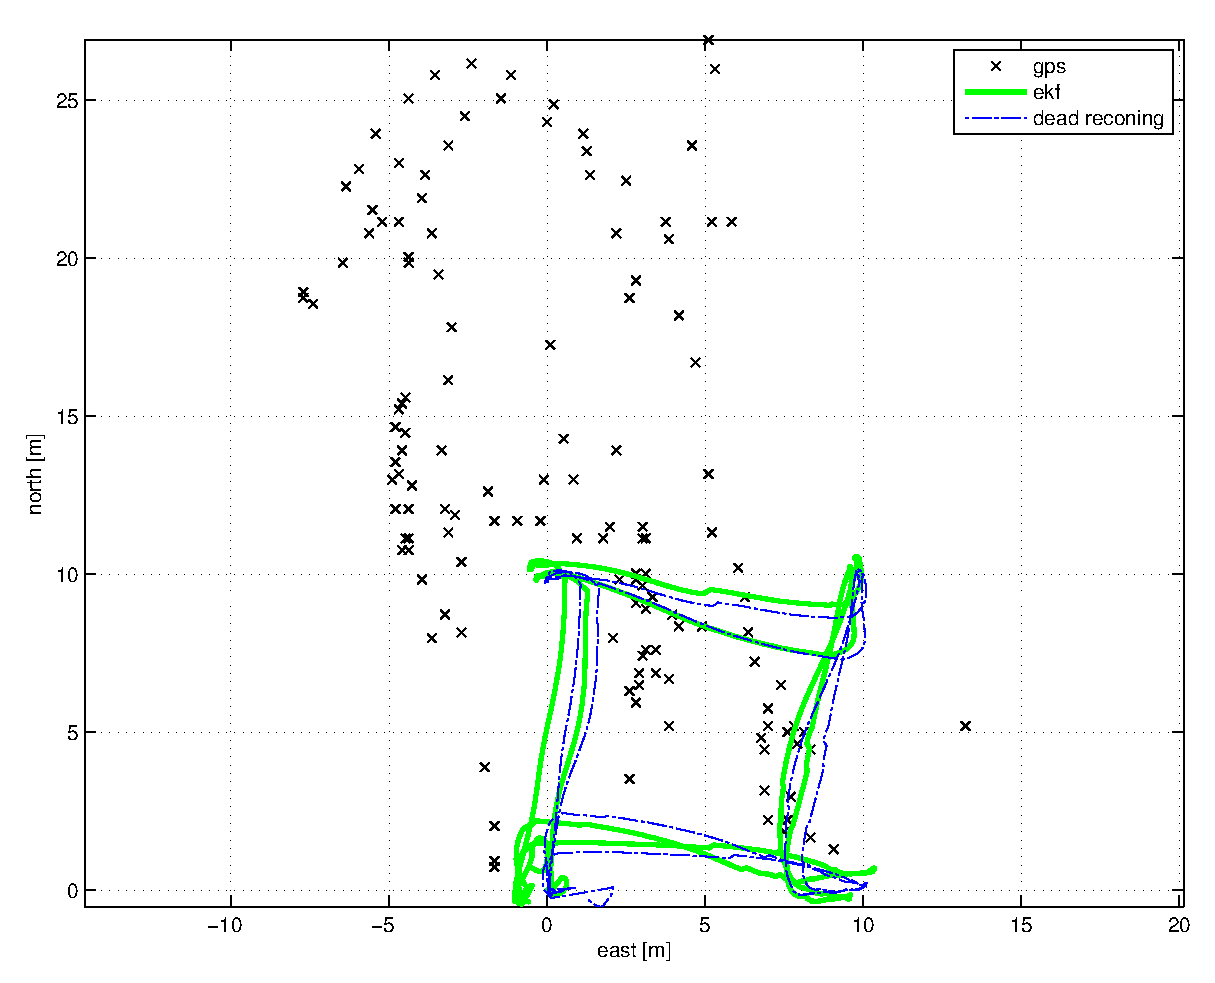
\includegraphics[width=0.48\linewidth]{results/fig/square2NoGps.eps}}\\
    %\subfigure[] {}
    %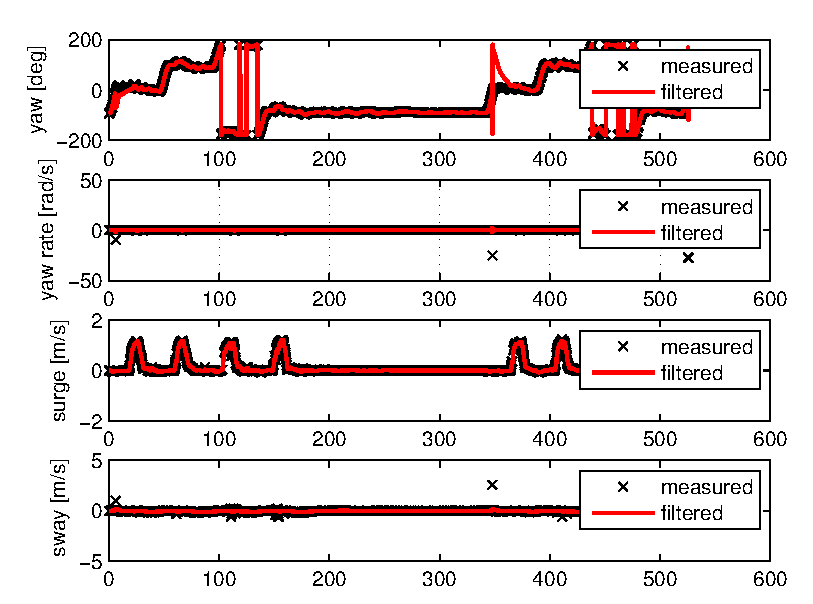
\includegraphics[width=0.6\linewidth]{results/fig/dynamics.eps}}
    \caption{EKF localisation using only inertial measurements as observation.}
    \label{fig:no-gps}
\end{figure}

\begin{figure}%[hb]%tb
  \centering
    \subfigure[Setting standard deviation of 1 m in uncertainty position observation (SDnorth = SDeast = 1.0 m).] {\label{fig:square-withGps-1}
	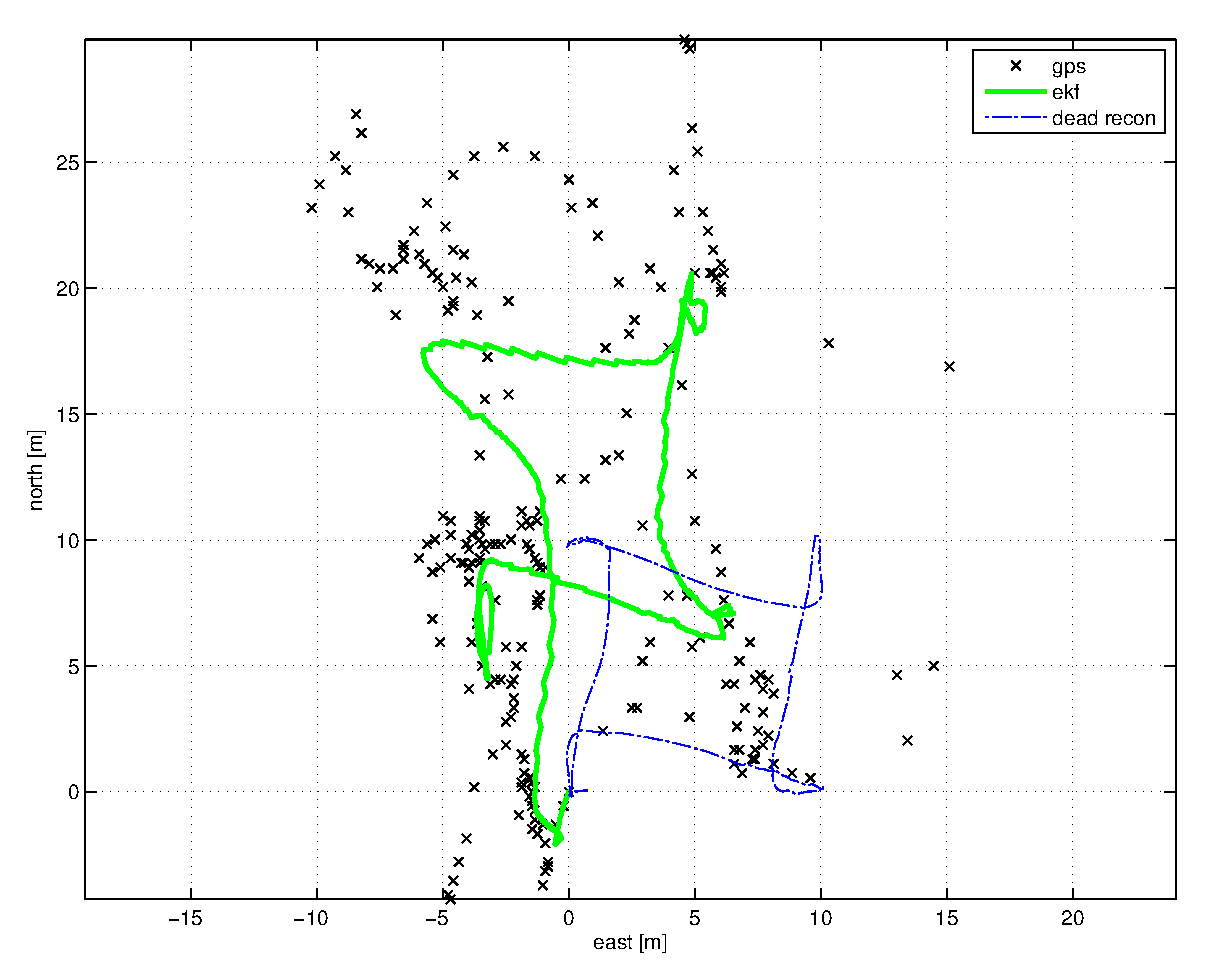
\includegraphics[width=0.48\linewidth]{results/fig/squareWithGps-10.eps}}
    \subfigure[EKF localisation after tuning the position uncertainty (SDnorth = SDeast = 0.5 m).] {\label{fig:square-withGps-2}
	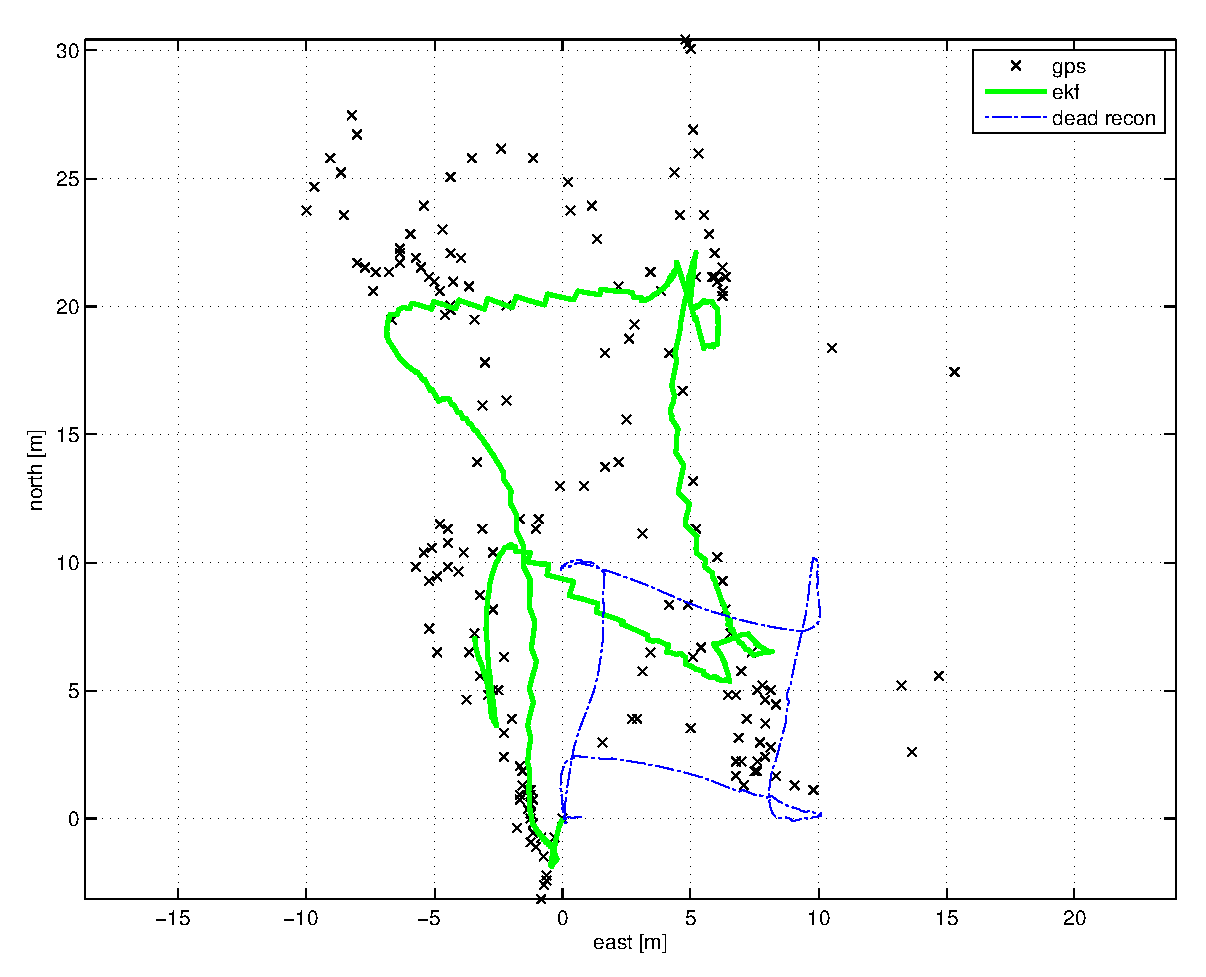
\includegraphics[width=0.48\linewidth]{results/fig/squareWithGps-05.eps}}
    %\\
    %\subfigure[Linear and angular velocities during square-shaped trajectory.] {\label{fig:square-dynamics}
    %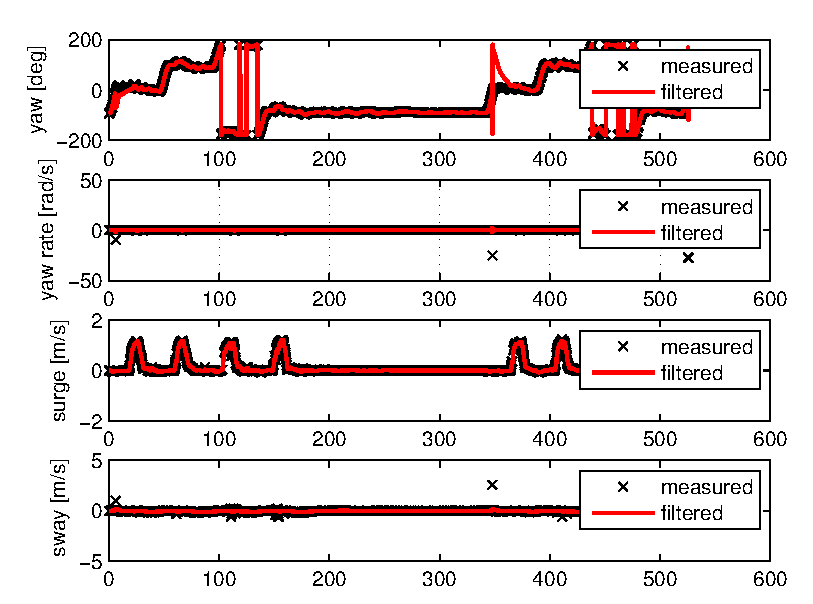
\includegraphics[width=0.45\linewidth]{results/fig/dynamics.eps}}
    \caption{EKF localisation aided with GPS position updates weighted by setting appropriate parameters.}
    \label{fig:with-gps}
\end{figure}
\begin{figure}
\centering
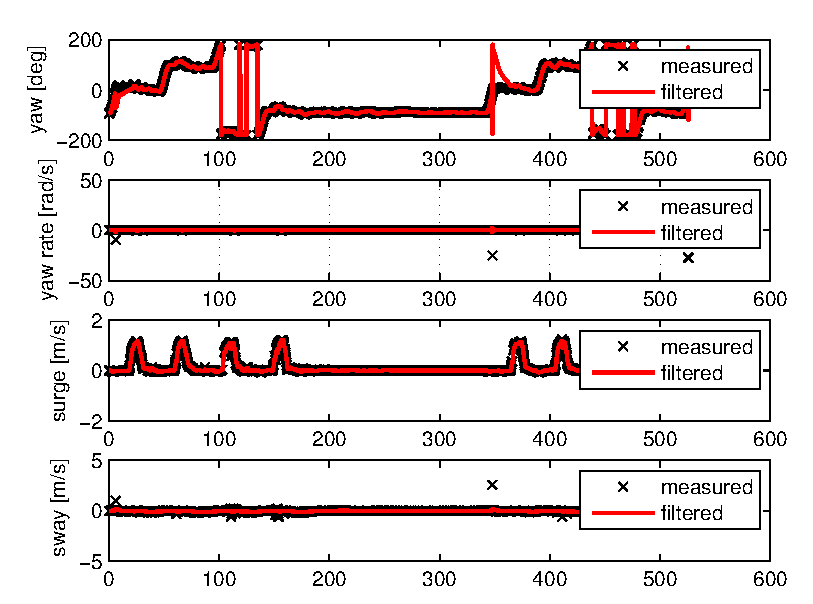
\includegraphics[width=0.6\linewidth]{results/fig/dynamics.eps}
\caption{Linear and angular velocities during square-shaped trajectory.}
\label{fig:square-dynamics}
\end{figure}
\T{With GPS: } Finally, GPS measurements were appended to the EKF observations. Localisation results were shown in Figure ~\ref{fig:with-gps} for two different level of confidence (variances) in position measurement. Naturally, giving extremely high confidence does not seem to be the best choice, however, some empirically deduced values in range of decimetres significantly correct the dead reckoning drift. Furthermore, EKF tends to filter the GPS measured north east coordinates, hence partially corrects the GPS imprecisions stated at the beginning. At this point it is evident why EKF is a great tool. Filter tries to satisfy the set uncertainty boundaries and fuse all the available information trying to make the most out of it combined together in one mathematical system. Moreover, fusing such imprecise and sketchy position data from GPS, still improves the localisation. Obtained trajectory tends to go towards what can be treated as expected path. From something that looked like a noisy collection of position observations at the beginning (Figure ~\ref{fig:gps-signal}), application of EKF together with sensor fusion enabled having generally better performance in navigation.     
%Combination of all relevant sensors gives in a Kalman filter state estimate results in more precise position and heading compared with instant (flat) usage of position and orientation measurements.  
%\subsection{Sensor selection}
%Design and performance test.
%\subsection{Using FOG for navigation improvement}
%How big is the improvement with respect to the distance travelled?

%\chapter{Conclusions} \label{chap:conclusions}
The main focus of the work presented in the thesis is practical application of Extended Kalman Filter (EKF) for Ocean System Lab's Nessie AUV navigation module. EKF was designed to estimate the location of an underwater robot by processing real-time inertial and position information obtained from sensors. Furthermore, EKF algorithm was utilized as a tool for accomplishing sensor fusion - blending together measurements from different sensors as a part of the estimation process. Some principles of implementation for EKF-based localisation that were already available in literature were adopted and modified into a five d.o.f. vehicle model.

One of the issues that were addressed in the thesis was the suitable management of measurement tasks among mounted sensor devices and the role of EKF in correcting deficiencies. Specific case of heading measurement was tested, since this type of angular information is particularly important for the navigation. Usage of magnetic compass for obtaining heading is possible, however needs serious and precise calibration of the compass on the location itself. Advantage would be the possibility to make corrections based on absolute but quite noisy an unstable heading information that can be filtered using EKF tuned to compensate for the magnetic compass inaccuracies. Due to calibration difficulties, most of the experiments use the magnetic compass for initial heading, and EKF successfully appends the accurate heading rate information obtained from gyroscope to compensate for the lack of absolute heading. 

In conclusion, EKF proves to be useful navigation tool with satisfactory navigation performance and several convenient features. Flexible with the number of sensors involved, capable of successfully combining together different sensory information into a location estimate that tends to be optimal with respect to set expectations, or recovering from the missing measurements, outliers, or noise. The issues with nonlinearity have been addressed and the usage of Unscented Kalman Filter (UKF) tested on real data. Implementation of UKF for localisation would improve the accuracy of approximating nonlinearities in EKF at the same computational cost. However, this would have impact on navigation quality in cases when process model is fairly similar to the real robot movement. Simply said - UKF will tune up the emulation of the mathematical equations (prediction). If the prediction mode has an important role in estimation, UKF will contribute. A possibility to test adopted UKF that randomly takes samples is an idea to cope with filtering noisy position information such as LBL's ``mutipathing'' or imprecisions.      

\section{Future work}
Future work on improving localisation performance involves more trials, particularly ones where the true trajectory has been fixed to known landmarks, so that the results of localisation could be thoroughly evaluated with trustful ground truth. Experiments that involve tilted vehicle movements could make an evaluation of the influence of the 5th degree of freedom on localisation. EKF could be modified so that it works with control inputs - which could contribute robustness of the localisation. 

Finally, the problem of correcting the absolute position with LBL information gives space for improvement since the measured position tends to be quite uncertain and prone to different sorts of noise. Solution for rejecting outliers could rely on some version of back-filtering - filtering based on history of received observations.          

%\appendix
%\chapter{The first appendix}
If you need to add any appendix, do it here...
 Etc.


%   this is for BibTeX.  remove if you plan to write the references in the document
\bibliographystyle{plain}
\bibliography{refs}


%adds the bibliography to the table of contents
\addcontentsline{toc}{chapter}
         {\protect\numberline{Bibliography\hspace{-96pt}}}

\end{document}